\documentclass[addpoints]{exam}
\usepackage[utf8]{inputenc}
\usepackage{amsmath}
\usepackage{mathtools}
\usepackage{relsize}
\usepackage{tikz}
\usepackage{pgfplots}
\usetikzlibrary{datavisualization}
\usetikzlibrary{datavisualization.formats.functions}
\usepackage{dirtytalk}
\usepackage{graphicx}
\graphicspath{ {./drift/} }
\newcommand\Mycomb[2][^n]{\prescript{#1\mkern-0.5mu}{}C_{#2}}
\DeclarePairedDelimiter{\ceil}{\lceil}{\rceil}
\usepackage{geometry}
\usepackage{draftwatermark}
\SetWatermarkFontSize{2cm}
\SetWatermarkText{DU - Mathematics}
\usepackage[banglamainfont=Kalpurush, 
            banglattfont=Siyam Rupali
           ]{latexbangla}

\lfoot{Sayma Mostafa}
\rhead{\thepage}
\rfoot{প্রমি}

          
\begin{document}
\begin{LARGE}
\begin{center}
গণিত (Mathematics - 2018)
\end{center}
\end{LARGE}
\begin{questions}

 \question  $ f(x) = 1+x^3 $ বক্ররেখাটির সাথে $ x- $ অক্ষের ছেদবিন্দুর সংখ্যা (The number of the intersection by the curve $ f(x) = 1+x^3 $ with the $ x- $axis is)

\begin{oneparchoices}
\choice 0
\choice 1
\choice 2
\choice 3

\end{oneparchoices}

\question  $ y = \dfrac{1+x}{1-x} $ হলে $ \dfrac{dy}{dx} $ এর মান (If $ y = \dfrac{1+x}{1-x} $ then, $ \dfrac{dy}{dx} $ equals)

\begin{oneparchoices}
\choice $ \dfrac{-2}{(x-1)^2} $
\choice $ \dfrac{2}{(1-x^2)} $
\choice $ \dfrac{2}{(1-x)^2} $
\choice $ \dfrac{2x}{(1-x)^2} $

\end{oneparchoices} 

\question  $ z= \dfrac{-4+3i}{i} $ এর কাল্পনিক অংশ (The imaginary part of $ z= \dfrac{-4+3i}{i} $ is )

\begin{oneparchoices}
\choice 3
\choice 4 
\choice $ -4 $
\choice  $ -3 $
\end{oneparchoices}

\question  $\Mycomb{1} + \Mycomb{2} +\Mycomb{3} + \cdots + \Mycomb{n} = ?$ 

\begin{oneparchoices}
\choice $ 2^{n} + 1 $
\choice $ 2^{n} $
\choice $ 2^{n-1} $
\choice  $ 2^{n} - 1 $
\end{oneparchoices}

\question  দুটি সমান মানের P বল এর সর্বনিন্ম লদ্ধি কত ?(What is the minimum resultant of two equal forces of magnitude P ?) 

\begin{oneparchoices}
\choice 2P
\choice 0
\choice P
\choice $ \dfrac{P}{2} $

\end{oneparchoices}


\question  একটি চলন্ত ট্রেনকে ব্রেক করে 10s এ থামিয়ে দেয়া হলো । ট্রেনটির গড় মন্দন $ 70m/sec^{2} $ হলে এর গতিবেগ কত ছিল? (A running train is stopped in seconds with a break. What was the velocity of train if its retardation was $ 70m/sec^{2} $ ?)

\begin{oneparchoices}
\choice 1000 m/sec
\choice  800 m/sec
\choice  700 m/sec
\choice  500 m/sec

\end{oneparchoices}

\question  $ 3x^{2} + 3y^{2} -5x-6y +4 =0 $ বৃত্তটির কেন্দ্র - (The center of the circle is  $ 3x^{2} + 3y^{2} -5x-6y +4 =0 $) 

\begin{oneparchoices}
\choice $ (1, \dfrac{2}{3})$
\choice $ (\dfrac{5}{6}, 1) $
\choice $ (\dfrac{5}{3}, 1) $
\choice $ (\dfrac{2}{3}, -1) $

\end{oneparchoices}

\question  $ y=ks $ সরলরেখাটি $ y = x^{2}+4 $ বক্ররেখার স্পর্শক হলে $ k $ এর একটি মান- (The straight line $ y=ks $ will be a tangent to the curve $ y = x^{2}+4 $ if one of the values of $ k $ is ) 

\begin{oneparchoices}
\choice 1
\choice $ 2\sqrt{2} $
\choice $ 3 $
\choice $ 4 $

\end{oneparchoices}

\question  $ y=2 $ এবং $ y=|x| $ রেখা দুটি দ্বারা আবদ্ধ ক্ষেত্রের ক্ষেত্রফল (The area bounded by the line $ y=2 $ and $ y=|x| $ is )

\begin{oneparchoices}
\choice 2 sq. units
\choice 4 sq. units
\choice 6 sq. units
\choice 8 sq. units

\end{oneparchoices}

\question  \say{Permutation}  শব্দটির বর্ণগুলোর মধ্যে স্বরবর্ণের অবস্থান পরিবর্তন না করে কতরকমে পুনরায় সাজানো যাবে? (How may ways the word \say{Permutation} can be rearranged without changing the position of the vowels ?)

\begin{oneparchoices}
\choice 360
\choice 460
\choice 459
\choice 359
\end{oneparchoices}


\question   120 জন ছাত্রের মধ্যে 75 জন ক্রিকেট খেলে এবং 65 জন ফুটবল খেলে। কতজন উভয় খেলাই খেলে? (Out of 120 students 75 play cricket and 65 play football. How many of them play both of the games ?)

\begin{oneparchoices}
\choice 10
\choice 20
\choice 30
\choice 45

\end{oneparchoices}

\question   $ \mathlarger{|3-\dfrac{1}{x}|<\dfrac{1}{2}} $ অসমতাটির সমাধান সেট (The solution set of the inequality $ \mathlarger{|3-\dfrac{1}{x}|<\dfrac{1}{2}} $ is )

\begin{oneparchoices}
\choice $ \dfrac{2}{7} < x < \dfrac{2}{5}$
\choice $ -\dfrac{4}{7} < x < -\dfrac{4}{5}$
\choice $ \dfrac{1}{8} < x < \dfrac{1}{7}$
\choice $ \dfrac{1}{5} > x > \dfrac{1}{7}$

\end{oneparchoices}

\question  $ \tan^{-1}\dfrac{2}{3} + \cos^{-1}\dfrac{2}{\sqrt{13}} = ?$

\begin{oneparchoices}
\choice $ \tan^{-1}\dfrac{5}{9} $ 
\choice $ \tan^{-1}\dfrac{3}{7} $ 
\choice $ \dfrac{\pi}{2} $ 
\choice $ \dfrac{\pi}{4} $ 

\end{oneparchoices}

\question  $ (x^{2} + \dfrac{2}{x})^{6} $ এর বিস্তৃতিতে $ x$ মুক্ত পদ- (The $ x $ free term in the expansion of $ (x^{2} + \dfrac{2}{x})^{6} $ is )

\begin{oneparchoices}
\choice 204
\choice 240 
\choice 402 
\choice 420 

\end{oneparchoices}

\question  $ \mathlarger{\int\sqrt{e^{x}}dx} =? $

\begin{oneparchoices}
\choice $ \dfrac{2}{3}(e^x)^{\frac{3}{2}} + c$ 
\choice $ \dfrac{1}{2}\sqrt{e^x} + c $
\choice $ 2e^{\frac{x}{2}} + c $
\choice $ e^{\frac{x}{2}} + c $

\end{oneparchoices}

\question  $ \mathlarger{\int\dfrac{\tan(\sin^{-1}x)}{\sqrt{1-x^{2}}} dx} =? $

\begin{oneparchoices}
\choice $ \sec^{2}(\sin^{-1}x) + c$ 
\choice $ \sec(\sin^{-1}x) + c $ 
\choice $ ln|\sec(\sin^{-1}x)| + c $
\choice $ ln|\tan(\sin^{-1}x)| + c $

\end{oneparchoices}

\question    4 থেকে 15 পর্যন্ত সংখ্যা হতে যেকোনো একটিকে দৈবচয়নের মাধ্যমে নিলে সেই সংখ্যাটি মৌলিক অথবা এর গুণিতক হওয়ার সম্ভাবনা কত? (What is the probability that a number chosen randomly from 4 to 15 is prime number or multiple of 3?)

\begin{oneparchoices}
\choice $ \dfrac{6}{7}$ 
\choice $ \dfrac{5}{12}$ 
\choice $ \dfrac{2}{3} $ 
\choice $ \dfrac{7}{12} $ 
\end{oneparchoices}

\question   $ f(x) = \dfrac{-1}{|1-x|} $  ফাংশনের রেঞ্জ (The range of the function $ f(x) = \dfrac{-1}{|1-x|} $ is)
 
\begin{oneparchoices}
\choice $ \mathbb{R}-{1} $
\choice $ \mathbb{R}-{0} $
\choice $ \mathbb{R}-{0,1} $
\choice  $ (-\infty, 0) $

\end{oneparchoices}

\question $ y=b $ এবং $ \sqrt{3}x-y+1=0 $ রেখাদ্বয়ের অর্ন্তভুক্ত সুক্ষকোণের মান (The acute angle between the straight line $ y=b $ and $ \sqrt{3}x-y+1=0 $ is ) 

\begin{oneparchoices}
\choice $ 30^{\circ} $
\choice $ 45^{\circ} $
\choice $ 60^{\circ} $
\choice $ 90^{\circ} $

\end{oneparchoices}


\question  ভেক্টর $ \vec{u} = \hat{i} + \hat{j} $ ও $ \vec{v} = \hat{j} + \hat{k} $ এর অন্তর্ভুক্ত কোণ (The angle between vector $ \vec{u} = \hat{i} + \hat{j} $ and  $ \vec{v} = \hat{j} + \hat{k} $ is)

\begin{oneparchoices}
\choice $ \cos^{-1}(\dfrac{1}{\sqrt{3}}) $
\choice $ \cos^{-1}(\dfrac{1}{3}) $
\choice $ \cos^{-1}(\dfrac{1}{2}) $
\choice $ \cos^{-1}(\dfrac{1}{\sqrt{2}}) $

\end{oneparchoices}

\question  $ x^{2} + y^{2}+2x-4y+4=0 $ বৃত্তের একটি স্পর্শক (One of the tangents to circle $ x^{2} + y^{2}+2x-4y+4=0 $ is ) 

\begin{oneparchoices}
\choice $ x =0 $
\choice $ x=2 $
\choice $ y=0 $
\choice  $ y=4 $

\end{oneparchoices}

\question  $ \cos^{2}(60^{\circ} + A) + \cos^{2}(60^{\circ} -A) $ এর মান (The value of  $ \cos^{2}(60^{\circ} + A) + \cos^{2}(60^{\circ} -A) $ is ) 

\begin{oneparchoices}
\choice $ 1-\dfrac{1}{2}\cos 2A $
\choice $ 1+\sin 2A $
\choice $ 1+3\cos 2A $ 
\choice $ 1-\dfrac{1}{2}\cos 2A $

\end{oneparchoices}

\question  $ 2r\sin^{2}(\dfrac{\theta}{2}) = 1 $ এর কার্তেসীয় সমীকরণ (The Cartesian equation of $ 2r\sin^{2}(\dfrac{\theta}{2}) $ is)

\begin{oneparchoices}
\choice $ y^{2} = 1+2x $
\choice $ y^{2} = 4(1-x) $
\choice $ y^{2} = 4(1+x) $
\choice $ x^{2} = 4(1+y) $

\end{oneparchoices}

\question   $ \cot\theta \cot 3\theta =1 $ সমীকরণের সাধারণ সমাধান  (The general solution of the equation $ \cot\theta \cot 3\theta =1 $ is)

\begin{oneparchoices}
\choice $ \dfrac{(2n+1)\pi}{4} $
\choice $ \dfrac{(2n+1)\pi}{8} $
\choice $ \dfrac{n\pi}{4} $
\choice  $ \dfrac{(2n-1)\pi}{2} $

\end{oneparchoices}

\question $ y=x+4 $  এবং $ y=x $  রেখাদ্বয়ের লম্বদুরত্ব (The perpendicular distance between the line $ y=x+4 $ and $ y=x $ is ) 

\begin{oneparchoices}
\choice 4 একক
\choice $2\sqrt{2}$ একক
\choice 2 একক
\choice  $ 4\sqrt{2} $ একক
\end{oneparchoices}

\question $ x = \dfrac{1}{2}(-1+\sqrt{-3}) $  এবং $ y = \dfrac{1}{2}(-1-\sqrt{-3})  $ হলে $ x^{2} + xy + y^{2} $ এর মান (If $ x = \dfrac{1}{2}(-1+\sqrt{-3}) $ and $ y = \dfrac{1}{2}(-1-\sqrt{-3})  $ then the value of  $ x^{2} + xy + y^{2} $ is )

\begin{oneparchoices}
\choice $ 0 $
\choice $ 2 $
\choice $ 1 + \sqrt{3} $
\choice  $ 1 $

\end{oneparchoices}

\question  $ y^{2}-4y-x^{2}+6x =12 $  সমীকরণটি কোন ধরনের কণিক? (The type of the conic $ y^{2}-4y-x^{2}+6x =12 $ is)

\begin{oneparchoices}
\choice বৃত্ত (Circle)
\choice উপবৃত্ত (Ellipse)
\choice পরাবৃত্ত (Parabola)
\choice  অধিবৃত্ত (Hyperbola)

\end{oneparchoices}

\question  $ 2x^{2}-8y^{2} = 2 $ অধিবৃত্তের উৎকেন্দ্রিকতার মান (The value of the eccentricity of the hyperbola $ 2x^{2}-8y^{2} = 2 $ is )

\begin{oneparchoices}
\choice $ \dfrac{3}{2\sqrt{2}} $
\choice $ \dfrac{3}{2} $
\choice $ \dfrac{\sqrt{5}}{2} $
\choice  $ \sqrt{\dfrac{5}{2}} $

\end{oneparchoices}

\question  $ \mathlarger{\lim_{x \to 0} \dfrac{\sin x}{\tan^{-1}(3x)}} $

\begin{oneparchoices}
\choice $ 0 $
\choice $ \dfrac{1}{3} $
\choice $ 1 $
\choice  $ 3 $

\end{oneparchoices}

\question   $ x^{2}-7x+2=0 $ সমীকরণের মূলদ্বয় হতে 2 কমমূল বিশিষ্ট সমীকরণটি (The equation whose roots are less by 2 than those of the equation $ x^{2}-7x+2=0 $ is)

\begin{oneparchoices}
\choice $ x^{2}-4x+6=0 $
\choice $ x^{2}-3x-8=0 $
\choice $ x^{2}-11x+8=0 $
\choice $ x^{2}-3x+8=0 $

\end{oneparchoices}

\end{questions}


\begin{LARGE}
\begin{center}
গণিত (Mathematics - 2017 )
\end{center}
\end{LARGE}
\begin{questions}

\question $ A=\begin{vmatrix}
a & 2 & 5 \\
-2 & b & -3 \\
-5 & 3 & c
\end{vmatrix} $  একটি বক্র প্রতিসম ম্যাট্রিক্স হলে $ a,\,b $ ও $ c $ এর মানগুলো (If $ A=\begin{vmatrix}
a & 2 & 5 \\
-2 & b & -3 \\
-5 & 3 & c
\end{vmatrix} $ is a skew symmetric matrix then the values of $ a,\,b $ and $ c $ are )

\begin{oneparchoices}
\choice  $-2,\, -5,\, 3$
\choice  $0,\, 0,\, 0$
\choice  $1,\, 1,\, 1$
\choice  $2,\, 5,\, 3$

\end{oneparchoices}

\question  $ k $ এর কোন মানের জন্য $ \begin{vmatrix}
1 & 1 & 1 \\
1 & k & k^2 \\
1 & k^2 & k^3
\end{vmatrix}  $ নির্ণায়কটির মান শূণ্য হবে না? (For which value of $ k $, the value of the  determinant $ \begin{vmatrix}
1 & 1 & 1 \\
1 & k & k^2 \\
1 & k^2 & k^3
\end{vmatrix}  $ is not zero ? )

\begin{oneparchoices}
\choice $ k=1 $
\choice $ k=-1 $
\choice $ k=3 $
\choice  $ k=0 $

\end{oneparchoices}
    

\question   অসমতা $ |5-2x|\ge 4 $ এর সমাধান সেট (The solution set of the  inequality $ |5-2x|\ge 4 $ is )

\begin{oneparchoices}
\choice $ \Big[ \dfrac{1}{2}, \dfrac{9}{2} \Big] $
\choice $ \Big(-\infty, \dfrac{1}{2} \Big] \cup \Big[\dfrac{9}{2}, \infty \Big)$ 
\choice $ \Big[ -\infty, \dfrac{1}{2} \Big] $
\choice  $ \Big[ \dfrac{1}{2}, \dfrac{9}{2} \Big]\cup \Big[ \dfrac{27}{2}, \infty \Big) $

\end{oneparchoices}

\question   যদি $z_{1}=1-i, \; z_{2} = \sqrt{3} +i $ হয় তবে $ \dfrac{z_{2}}{z_{1}} $ এর নতি ( If $z_{1}=1-i, \; z_{2} = \sqrt{3} +i $, then the argument of $ \dfrac{z_{2}}{z_{1}} $ is )

\begin{oneparchoices}
\choice $ \dfrac{5\pi}{12} $
\choice $ \dfrac{\pi}{6} $
\choice $ -\dfrac{\pi}{4} $
\choice $ -\dfrac{5\pi}{12} $

\end{oneparchoices}


\question  কোন দ্বিঘাত সমীকরণের একটি মূল $ \dfrac{1}{1+i} $ হলে সমীকরণটি হবে (If one root of a quadratic equation is $\dfrac{1}{1+i}$, then the equation is )

\begin{oneparchoices}
\choice $ x^2 -x +1=0 $
\choice $ 2x^2 -2x +1=0 $
\choice $ x^2 +x +1=0 $
\choice $ 2x^2 +2x +1=0 $

\end{oneparchoices}

\question  RAJSHAHI শব্দটির অক্ষরগুলির একত্রে বিন্যাস সংখ্যা BARISHAL শব্দটির অক্ষরগুলির বিন্যাস সংখ্যার $ k $ গুণ হলে $ k $ এর মান (If the permutation by taking all the letters of RAJSHAHI is $ k $ times of the permutation by taking all the letters of BARISHAL, then the value of $ k $ is)

\begin{oneparchoices}
\choice $ 2$
\choice $ 3$
\choice $ 4$
\choice $ 5$

\end{oneparchoices}

\question  $ \Big(x-\dfrac{1}{x}\Big)^{16} $  এর  বিস্তৃতিতে মধ্যপদটি হবে (The middle term of the expansion of $ \Big(x-\dfrac{1}{x}\Big)^{16} $ is )

\begin{oneparchoices}
\choice $ 12780 $
\choice $ 42708 $
\choice $ 12870 $
\choice $ 12807 $

\end{oneparchoices}

\question $ 1+\dfrac{1}{3} + \Big( \dfrac{1}{3}\Big)^2+ \Big( \dfrac{1}{3}\Big)^3 +\cdots $  অসীম পর্যন্ত এর মান (The value of $ 1+\dfrac{1}{3} + \Big( \dfrac{1}{3}\Big)^2+ \Big( \dfrac{1}{3}\Big)^3 +\cdots $ up to infinity is )

\begin{oneparchoices}
\choice $ \dfrac{2}{3} $
\choice $ \dfrac{3}{2} $
\choice $ \dfrac{1}{3} $
\choice $ \dfrac{1}{2} $

\end{oneparchoices}

\question  $ \vec{a} = 4\hat{i}-3\hat{j} +2\hat{k} $ ও $ \vec{b} = 2\hat{i}-3\hat{j} +4\hat{k} $ ভেক্টর দুইটি যে সামান্তরিকের সন্নিহিত বাহু তার ক্ষেত্রফল হবে (The area of the parallelogram having $ \vec{a} = 4\hat{i}-3\hat{j} +2\hat{k} $ and  $ \vec{b} = 2\hat{i}-3\hat{j} +4\hat{k} $ as the adjacent side is)

\begin{oneparchoices}
\choice $3\sqrt{3}$ sqrt units
\choice $6\sqrt{3}$ sqrt units
\choice $ 6\sqrt{6} $ sqrt units
\choice $ 3\sqrt{6} $ sqrt units

\end{oneparchoices}


\question   ভেক্টর  $ \vec{u} = 2\hat{i}+\hat{j} -3\hat{k} $ ও  $ \vec{v} = 3\hat{i}-2\hat{j} -\hat{k} $ এর অন্তর্ভুক্ত কোণ (The angle between vector  $ \vec{u} = 2\hat{i}+\hat{j} -3\hat{k} $ and $ \vec{v} = 3\hat{i}-2\hat{j} -\hat{k} $ is)

\begin{oneparchoices}
\choice $ 60^{\circ} $
\choice $ 45^{\circ} $
\choice $ 30^{\circ} $
\choice $ 120^{\circ} $

\end{oneparchoices}

\question  P(2,5), Q(5,9) এবং S(6,8) বিন্দুত্রয় PQRS রম্বসের শীর্ষবিন্দু হলে R এর স্থানাংক ( P(2,5), Q(5,9) and S(6,8) are three vertices of a rhombus PQRS, then the coordinates of R is )

\begin{oneparchoices}
\choice $ (12,\,9) $
\choice $ (\dfrac{7}{2},\, 7) $
\choice $ (4,\, \dfrac{13}{2}) $
\choice $ (9,12) $

\end{oneparchoices}


\question  মূলবিন্দুগামী একটি বৃত্ত ধনাত্নক $ x- $অক্ষহতে 4 একক এবং ধনাত্নক $ y- $অক্ষহতে 2 একক ছেদক কর্তন করলে, এর সমীকরণ হবে(The equation of the circle which passes through the origin and cuts off intercepts 4 and 2 units from the positive sides of $ x $ and $ y $ axis respectively is)

\begin{oneparchoices}
\choice $ x^2 + y^2 -4x-2y=0 $
\hspace*{1cm}\choice $ x^2 + y^2 +4x+2y=0 $\\
\hspace*{-.3cm}\choice $ x^2 + y^2 +2x+4y=0 $
\hspace*{1cm}\choice $ x^2 + y^2 -2x-4y=0 $

\end{oneparchoices}

\question  $ 25x^2 + 16y^2 = 400 $ এর উৎকেন্দ্রিকতা হবে (The eccentricity of $ 25x^2 + 16y^2 = 400 $ is)

\begin{oneparchoices}
\choice $ \dfrac{3}{5} $
\choice $ \dfrac{3}{4} $
\choice $ \dfrac{4}{5} $
\choice $ \dfrac{2}{3} $

\end{oneparchoices}

\question  $ y- $অক্ষের সমান্তরাল এবং $ 2x-7y+11=0 $ ও $ x+3y=8 $ রেখাদ্বয়ের ছেদবিন্দুদিয়ে অতিক্রমকারী সরলরেখার সমীকরণ(The equation of the straight line parallel to $y-$axis and passing through the point of intersection of the lines $ 2x-7y+11=0 $ and $ x+3y=8 $ is)

\begin{oneparchoices}
\choice $ 13x-23=0 $
\choice $ 3x-7=0 $
\choice $ 7x-3=0 $
\choice $ 23x-13=0 $

\end{oneparchoices}

\question $ A+B = \dfrac{\pi}{2} $  হলে $ \cos^{2}A - \cos^{2}B $ এর মান (If $ A+B = \dfrac{\pi}{2} $, then the value of $ \cos^{2}A - \cos^{2}B $ is)

\begin{oneparchoices}
\choice $ \sin (A-B) $
\choice $ \sin (B-A) $
\choice $ \cos (B-A) $
\choice $ -\cos (A-B) $

\end{oneparchoices}

\question  $ 0\le x\le 90^{\circ} $ হলে $ \sin 3x = \cos x $ সমীকরণের সমাধান হবে (If $ 0\le x\le 90^{\circ} $ then the solution of the equation $ \sin 3x = \cos x $ is)

\begin{oneparchoices}
\choice $ 0^{\circ},\, 45^{\circ} $
\choice $ 0^{\circ},\, 22.5^{\circ} $
\choice $ 45^{\circ},\,45^{\circ} $
\choice $ 22.5^{\circ},\, 45^{\circ}  $

\end{oneparchoices}

\question  $ \sin^{-1}x + \sin^{-1}y = \dfrac{\pi}{2} $ হলে কোনটি সঠিক? (If $ \sin^{-1}x + \sin^{-1}y = \dfrac{\pi}{2} $, then which one is correct?)

\begin{oneparchoices}
\choice $ x^2 + y^2 =1 $
\choice $ x^2 - y^2 =1 $
\choice $ x + y =1 $
\choice $ x-y=1  $

\end{oneparchoices}

\question   $ f(x) = \dfrac{1}{\sqrt{|x|}} $ এর ডোমেন (The domain of  $ f(x) = \dfrac{1}{\sqrt{|x|}} $ is)

\begin{oneparchoices}
\choice $ [0,+\infty) $
\choice $ (0,+\infty) $
\choice $ (-\infty, +\infty) $
\choice $ (-\infty, 0)\cup (0, +\infty)  $

\end{oneparchoices}

\question   $ \lim\limits_{x\to \infty} \dfrac{2x^2 +3x+5}{3x^2 +5x-6} $ এর মান (The value of $ \lim\limits_{x\to \infty} \dfrac{2x^2 +3x+5}{3x^2 +5x-6} $ is)

\begin{oneparchoices}
\choice $ \dfrac{3}{5} $
\choice $ -\dfrac{5}{6} $
\choice $ \dfrac{2}{3} $
\choice $ -\dfrac{2}{3}  $

\end{oneparchoices}

\question   $ f(x) = \sqrt{x-1} $ হলে $ f^{-1}(2) $ এর মান (If $ f(x) = \sqrt{x-1} $, then the value of $ f^{-1}(2) $ is)

\begin{oneparchoices}
\choice $ -1 $
\choice $ 3 $
\choice $ 1 $
\choice $ 5  $

\end{oneparchoices}

\question    $ (4,3) $ বিন্দুতে $ 3x^2 -4y^2 =12 $ অধিবৃত্তের স্পর্শকের ঢালের মান (The value of the slope of the tangent at the point $ (4,3) $ of the hyperbola $ 3x^2 -4y^2 =12 $ is)

\begin{oneparchoices}
\choice $ -1 $
\choice $ 1 $
\choice $ \dfrac{3}{4} $
\choice $ \dfrac{4}{3} $

\end{oneparchoices}

\question  $ x^{4}-4x^{3}+4x^{2} + 5  $  এর লঘিষ্ঠ মান (The minimum value of $ x^{4}-4x^{3}+4x^{2} + 5  $ is )

\begin{oneparchoices}
\choice $ 4 $
\choice $ 5 $
\choice $ 6 $
\choice $ 8 $

\end{oneparchoices}

\question  যদি $ \mathlarger{\int\limits_{0}^{6}}f(t)dt =8 $ হয় তবে $ \mathlarger{\int\limits_{0}^{3}}f(2x)dx $ এর মান (If $ \mathlarger{\int\limits_{0}^{6}}f(t)dt =8 $, then the value of $ \mathlarger{\int\limits_{0}^{3}}f(2x)dx $ is)

\begin{oneparchoices}
\choice $ 0 $
\choice $ 6 $
\choice $ 10 $
\choice $ 4 $

\end{oneparchoices}

\question  $ \mathlarger{\int \dfrac{dx}{x\sqrt{x^2 -1}} = f(x)+c} $  হলে $ f(x) $ সমান (If $ \mathlarger{\int \dfrac{dx}{x\sqrt{x^2 -1}} = f(x)+c} $, then $f(x)$ is equal ) 

\begin{oneparchoices}
\choice $ \sin x $
\choice $ \sin^{-1}x $
\choice $ \cos x $
\choice $ \sec^{-1} x $

\end{oneparchoices}


\question $ \mathlarger{\int\limits_{-1}^{1}|x|dx} $ এর মান (The value of $ \mathlarger{\int\limits_{-1}^{1}|x|dx} $ ) 

\begin{oneparchoices}
\choice $ 2 $
\choice $ -1 $
\choice $ 1 $
\choice $ 0 $

\end{oneparchoices}

\question $ y=x^2,\,x=1,\,x=3 $ এবং $ x- $অক্ষ দ্বারা সীমাবদ্ধ ক্ষেত্রের ক্ষেত্রফল (The area bounded by $ y=x^2,\,x=1,\,x=3 $ and $ x- $axis is)

\begin{oneparchoices}
\choice $ \dfrac{26}{3} $ sq units
\choice $ \dfrac{80}{3} $ sq units
\choice $ \dfrac{8}{3} $ sq units
\choice $ \dfrac{35}{3} $ sq units

\end{oneparchoices}

\question   $ x+2y\le 10,\, x+y\le 6,\, x\le 4,\, x,y\ge 0 $ শর্তাধীনে $ z= 2x+3y $ এর সর্বোচ্চ মান (The maximum value of $ z= 2x+3y $ subjected to $ x+2y\le 10,\, x+y\le 6,\, x\le 4,\, x,y\ge 0 $ is )

\begin{oneparchoices}
\choice 14
\choice 15
\choice 16
\choice 18

\end{oneparchoices}

\question   2N এবং 5N  মানের দুটি বল একই দিকে ক্রিয়ারত। উহাদের সর্বাধিক  লদ্ধি হবে (Two forces of magnitude 2N and 5N act on a same line in the same direction, then the maximum magnitude of the resultant is )

\begin{oneparchoices}
\choice 7N
\choice 3N
\choice $\sqrt{29}$N
\choice 5N

\end{oneparchoices}

\question   যদি $ u $ বেগে অনুভূমিকের সাথে $ \alpha $ কোণে প্রক্ষিপ্ত বস্তু $ T $ সময়ে তার গতিপথের সর্বোচ্চ উচ্চতা $ H $ এ পৌঁছায় তবে $ \dfrac{H}{T^2} $ হবে (If the greatest height $ H $ is attained in time $ T $ by a body projected with  a velocity $ u $ at an angle $ \alpha $, then $ \dfrac{H}{T^2} is $  )

\begin{oneparchoices}
\choice $ \dfrac{2}{g} $
\choice $ \dfrac{g}{2} $
\choice $ g $
\choice $ \dfrac{1}{g} $

\end{oneparchoices}

\question  1  হতে 99 পর্যন্ত সংখ্যাগুলো থেকে দৈবচয়ন পদ্ধতিতে একটি সংখ্যা নেয়া হলে সেটি বর্গ হওয়ার সম্ভাবনা হবে (If a number randomly from 1 to 99, then the probability that it would be a square is) 

\begin{oneparchoices}
\choice $ \dfrac{1}{9} $
\choice $ \dfrac{2}{9} $
\choice $ \dfrac{1}{11} $
\choice $ \dfrac{2}{11} $

\end{oneparchoices}

\end{questions}
\begin{LARGE}
\begin{center}
গণিত (Mathematics - 2016)
\end{center}
\end{LARGE}
\begin{questions}

 \question $ |x^2 +1|<10 $  এর সমাধান (Solution of $ |x^2 +1|<10 $ is)

\begin{oneparchoices}
\choice $ -3<x<3 $
\choice $ -3\le x < 3 $
\choice $ -3<x \le 3 $
\choice $ -3 \le x \le 3 $

\end{oneparchoices}

\question  $ 5x -7y -15=0 $ সরলরেখার উপর লম্ব এবং $ (2,-3) $ বিন্দুগামী সরলরেখার সমীকরণ হবে (The equation of the straight line passing through the point $ (2,-3) $ and perpendicular to the straight line $ 5x-7y-15=0 $ is)

\begin{oneparchoices}
\choice $ 7x-5y-29=0 $
\choice $ 5x-7y-31=0 $
\choice $ 5x+7y+11=0 $
\choice  $ 7x+5y+1=0 $

\end{oneparchoices}

\question  $ y- $ অক্ষকে $ (0,4) $ বিন্দুতে স্পর্শ করে এবং কেন্দ্র $ 5x-7y-2=0 $ রেখার উপর অবস্থিত বৃত্তের সমীকরণ হবে (The equation of the circle touching $ y- $ axis at $ (0,4) $ and centre lying on the line $ 5x-7y-2=0 $ is)

\begin{oneparchoices}
\choice $ x^2 +y^2 + 12x-8y+16=0 $
\choice $ x^2 +y^2 -8x-6y+8=0 $ \\
\hspace*{-.45cm} \choice $ x^2 +y^2 - 12x-8y+16=0 $
\choice  $ x^2 +y^2 + 8x +6y-40=0 $

\end{oneparchoices}

\question  $ 2x +3y -4=0 $ এবং $ x\cos\alpha +y\sin\alpha= p$ একই সরলরেখা নির্দেশ করলে $ p $ এর মান ($ 2x +3y -4=0 $ and $ x\cos\alpha +y\sin\alpha= p$ represents the same line then the value of $ p $ is )

\begin{oneparchoices}
\choice $ \dfrac{1}{\sqrt{13}} $
\choice $ \dfrac{2}{\sqrt{13}} $
\choice $ \dfrac{3}{\sqrt{13}} $
\choice $ \dfrac{4}{\sqrt{13}} $

\end{oneparchoices}


\question  $ x=a $ এবং $ \sqrt{3}x-y+1=0 $ রেখাদ্বয়ের মধ্যবর্তী সূক্ষ্মকোণ (The acute angle between the straight lines $ x=a $ and $ \sqrt{3}x-y+1=0 $ )

\begin{oneparchoices}
\choice $ 30^{\circ} $
\choice $ 45^{\circ} $
\choice $ 60^{\circ} $
\choice $ 75^{\circ} $

\end{oneparchoices}

\question  সমাধান কর(Solve:) $ \sec^{2}\theta + \tan^{2}\theta = \dfrac{5}{3}, 0<\theta<\pi $

\begin{oneparchoices}
\choice $ -\dfrac{\pi}{6}, -\dfrac{5\pi}{6} $
\choice $ -\dfrac{\pi}{6}, \dfrac{5\pi}{6} $
\choice $ \dfrac{\pi}{6}, -\dfrac{5\pi}{6} $
\choice $ \dfrac{\pi}{6}, \dfrac{5\pi}{6} $

\end{oneparchoices}

\question   $ \sin (A-30^{\circ}) + \sin (150^{\circ} +A) $ এর মান (The value of $ \sin (A-30^{\circ}) + \sin (150^{\circ} +A) $ is)

\begin{oneparchoices}
\choice $ -\dfrac{1}{2}\cos A$
\choice $ 0 $
\choice $ \cos A $
\choice $ \sin A $

\end{oneparchoices}

\question   $ 4x^{2} + y^{2} = 2 $ উপবৃত্তটির বৃহৎ ও ক্ষুদ্র অক্ষের দৈর্ঘ্য যথাক্রমে (The length of major and minor axes of the ellipse $ 4x^{2} + y^{2} = 2 $ are respectively)

\begin{oneparchoices}
\choice 4 and 2
\choice 2 and 4
\choice $ \sqrt{2}$ and $ 2\sqrt{2} $
\choice $ 2\sqrt{2}$ and $ \sqrt{2} $

\end{oneparchoices}

\question   $ \mathlarger{\lim_{x \to 0}} \dfrac{e^{\cos x}}{\cos x} $ এর মান (The value of $ \mathlarger{\lim_{x \to 0}} \dfrac{e^{\cos x}}{\cos x} $ is)

\begin{oneparchoices}
\choice $e$
\choice $1 $
\choice $ \dfrac{1}{e} $
\choice $ 0 $

\end{oneparchoices}


\question   $ \mathlarger{\int\limits_{1}^{4}} f(x)dx=5$ হলে $ \mathlarger{\int\limits_{1}^{4}} f(3x+1)dx$ এর মান (If $ \mathlarger{\int\limits_{1}^{4}} f(x)dx=5$ then the value of $ \mathlarger{\int\limits_{1}^{4}} f(3x+1)dx$ is )

\begin{oneparchoices}
\choice $\dfrac{5}{4}$
\choice $ \dfrac{4}{3} $
\choice $ \dfrac{5}{3} $
\choice $ 5 $

\end{oneparchoices}

\question   $ y=x,\, y=0 $ রেখাদ্বয় এবং $ x^2 + y^2 =16 $ বৃত্তদ্বারা প্রথম চর্তুভাগে আবদ্ধ ক্ষেত্রের ক্ষেত্রফল (The area bounded in the first quadrant by the straight lines $ y=x,\, y=0 $ and the circle $ x^2 + y^2 =16 $ is)

\begin{oneparchoices}
\choice $ 2\pi$ sq. units
\choice $ 3\pi $ sq.units
\choice $ 4\pi $ sq.units
\choice $ 5\pi $ sq.units

\end{oneparchoices}

\question  $ f(x) = \sin x $ এবং $ g(x) = x^2 $ হলে $ (f\circ g)(\dfrac{\pi}{2}) $ এর মান হবে (If $ f(x) = \sin x $ and $ g(x) = x^2 $, then the value of $ (f\circ g)(\dfrac{\pi}{2}) $ is)

\begin{oneparchoices}
\choice $ \dfrac{1}{\sqrt{2}}$ 
\choice $ \dfrac{1}{2} $ 
\choice $ \dfrac{\sqrt{3}}{2} $ 
\choice $ \sqrt{2} $ 

\end{oneparchoices}

\question    যদি $ y=\sin^{-1}(\sin x) $ হয়,  তবে $ \dfrac{dy}{dx} $ হবে (If $ y=\sin^{-1}(\sin x) $, then $ \dfrac{dy}{dx} $ is )

\begin{oneparchoices}
\choice $ \sin x$ 
\choice $ \cos x $ 
\choice $ x $ 
\choice $ 1 $ 

\end{oneparchoices}

\question    $ x $ এর কোন মানের জন্য $ y= x+ \dfrac{1}{x} $ বক্ররেখাটির ঢাল শূণ্য হবে? (For what values of $ x $, the slope of the curve $ y= x+ \dfrac{1}{x} $ is zero?)

\begin{oneparchoices}
\choice $ x=\pm 2 $
\choice $ 1 $
\choice $ \pm 1 $
\choice  $ \pm \dfrac{3}{2} $

\end{oneparchoices}

\question $ y^2 +4x+2y-8=0 $  পরাবৃত্তের শীর্ষবিন্দু হবে (The vertex of the parabola $ y^2 +4x+2y-8=0 $ is)

\begin{oneparchoices}
\choice $ \Big( \dfrac{9}{4}, -1\Big) $
\choice $ \Big(- \dfrac{9}{4}, 1\Big) $
\choice $ (0,2) $
\choice  $ (2,0) $

\end{oneparchoices}


\question  $ \vec{P} = 5\hat{i}-3\hat{j}+2\hat{k} $  ভেক্টরের উপর $ \vec{Q} = 2\hat{i}+\hat{j}-2\hat{k} $ ভেক্টরের অভিক্ষেপ (The projection of $ \vec{Q} = 2\hat{i}+\hat{j}-2\hat{k} $ on $ \vec{P} = 5\hat{i}-3\hat{j}+2\hat{k} $ is)

\begin{oneparchoices}
\choice $ \dfrac{5}{\sqrt{38}} $
\choice $ \dfrac{3}{\sqrt{38}} $
\choice $ \dfrac{2}{\sqrt{38}} $
\choice  $ \dfrac{1}{\sqrt{38}} $

\end{oneparchoices}


\question  32 ft/s  আদিবেগ এবং ভূমি সাথে $ 30^{\circ} $ কোণে একটি বস্তু নিক্ষেপ করা হলো। ইহার ভ্রমণকাল (A particle is projected with an initial velocity 32 ft/s at an angle $ 30^{\circ} $ with the horizon. Tis time of flight is)

\begin{oneparchoices}
\choice 0.5 s
\choice 1 s
\choice 1.5 s
\choice  2 s

\end{oneparchoices}

\question   একটি সমবাহু ত্রিভুজের বাহুত্রয়ের সমান্তরালে একইক্রমে সমবিন্দুতে কার্যরত 6, 10, 14 একক মানের তিনটি বেগের লদ্ধির মান হবে (The magnitude of the resultant of the three velocities of 6, 10, 14 units acting at a point along three sides of an equilateral triangle in the same sense is)

\begin{oneparchoices}
\choice $ 4\sqrt{3} $ units
\choice $ 7\sqrt{3} $ units
\choice $ 10\sqrt{3} $ units
\choice  $ 15\sqrt{3} $ units

\end{oneparchoices}

\question   $ z=x+iy $ হলে $ |z-5| + |z+5| = 16 $ নির্দেশ করে (If $ z=x+iy $, then $ |z-5| + |z+5| = 16 $ represents)

\begin{oneparchoices}
\choice Circle
\choice Parabola
\choice Hyperbola
\choice Ellipse

\end{oneparchoices}

\question  $ \dfrac{1}{a+i} = \dfrac{i}{a-i} $  হলে $ a $ এর মান (If $ \dfrac{1}{a+i} = \dfrac{i}{a-i} $, then the value of $ a $ is)

\begin{oneparchoices}
\choice $ 1 $
\choice $ \dfrac{i}{2} $
\choice $ -1 $
\choice  $ -\dfrac{i}{2} $

\end{oneparchoices}

\question     1, 2, 0  দ্বারা গঠিত তিন অঙ্কবিশিষ্ট সংখ্যাগুলির মধ্যে কয়টি সংখ্যা 2 দ্বারা বিভাজ্য? (How many three digit numbers formed by 1, 2, 0 are divisible by 2?)

\begin{oneparchoices}
\choice 6
\choice 18
\choice 4
\choice  12

\end{oneparchoices}

\question   $ 3x^3 -1=0 $  এর মূলগুলি $ \alpha, \beta, \gamma $ হলে $ \alpha^{3} + \beta^{3} + \gamma^{3} $ এর মান (If $ \alpha, \beta, \gamma $ are the roots of $ 3x^3 -1=0 $, then the value of $ \alpha^{3} + \beta^{3} + \gamma^{3} $ is)

\begin{oneparchoices}
\choice $ -1 $
\choice $ 0 $
\choice $ \dfrac{1}{3} $
\choice  $ 1 $

\end{oneparchoices}

\question   $ \Bigg( 2x^2 -\dfrac{1}{2x^3}\Bigg)^{10} $   এর বিস্তৃতিতে বর্জিত পদের মান (The term independent of $ x $ in the expansion of $ \Bigg( 2x^2 -\dfrac{1}{2x^3}\Bigg)^{10} $ is )

\begin{oneparchoices}
\choice 540
\choice 640
\choice 740
\choice  840

\end{oneparchoices}

\question    'Mathematics' শব্দটির বর্ণগুলিকে কতরকমে সাজানো যাবে যেখানে প্রথমে ও শেষ স্থানে 'T' থাকবে (In how many ways the letters of the word 'Mathematics' can be arranged when first and last place will be fixed for 'T'?)

\begin{oneparchoices}
\choice 10080
\choice 9680
\choice 50720
\choice  90720

\end{oneparchoices}

\question  $ \dfrac{3x-1}{(x+1)(x^2 +1)} \equiv \dfrac{A}{x+1} + \dfrac{Bx+1}{x^2 +1} $  অভেদে (A,B) এর মান হবে (In the identity (A, B) equals)

\begin{oneparchoices}
\choice $ (-2,-2) $
\choice $ (-2, 2) $
\choice $ (2,-2) $
\choice  $ (2,2) $

\end{oneparchoices}

\question    $ A= \{1,2,3,5,9\} $ এবং $ B= \{1,2,9, 10\} $ হলে $ (A\setminus B)\cup (B\setminus A) $ এর সমান হবে (If $ A= \{1,2,3,5,9\} $ and $ B= \{1,2,9, 10\} $, then $ (A\setminus B)\cup (B\setminus A) $ equals)

\begin{oneparchoices}
\choice $ \{3,5\} $
\choice $ \{1,2,9\} $
\choice $ \{3,5, 10\} $
\choice  $ \{1,2,3,5,9,10\} $

\end{oneparchoices}

\question  $ \dfrac{1}{2}(e^{x}-e^{-x}) $   ধারাটির বিস্তৃতি কি? (What is the expansion of the series  $ \dfrac{1}{2}(e^{x}-e^{-x}) $ ? )

\begin{oneparchoices}
\choice $ x-\dfrac{x^{3}}{3!} +\dfrac{x^{5}}{5!}-\cdots$
\choice $ x+\dfrac{x^{3}}{3!} +\dfrac{x^{5}}{5!}+\cdots$
\choice $ 1+x+\dfrac{x^{3}}{3!} +\dfrac{x^{5}}{5!}+\cdots$
\choice  $ -x-\dfrac{x^{3}}{3!} -\dfrac{x^{5}}{5!}-\cdots$

\end{oneparchoices}

\question   যদি $ 9\theta = \pi $ হয়, তবে $ \cos\theta\cos 2\theta \cos 4\theta $ এর মান (If $ 9\theta = \pi $, then the value of $ \cos\theta\cos 2\theta \cos 4\theta $ is)

\begin{oneparchoices}
\choice $ \dfrac{1}{9} $
\choice $ \dfrac{1}{8} $
\choice $ 8 $
\choice  $ 9 $

\end{oneparchoices}

\question  $ \tan^{-1}\Bigg(x+\dfrac{1}{3}\Bigg) \tan^{-1}\Bigg(x-\dfrac{1}{3}\Bigg) =\tan^{-1}2 $  হলে $ x $ এর মান (If $ \tan^{-1}\Bigg(x+\dfrac{1}{3}\Bigg) \tan^{-1}\Bigg(x-\dfrac{1}{3}\Bigg) =\tan^{-1}2 $, then the value of $ x $ is)

\begin{oneparchoices}
\choice $ -\dfrac{5}{6} $
\choice $ -\dfrac{1}{3} $
\choice $ \dfrac{1}{3} $
\choice  $ \dfrac{2}{3} $

\end{oneparchoices}

\question   একটি বাক্সে 3টি লাল, 3টি সবুজ 2টি নীল বল আছে। দৈবভাবে 3টি বল তোলা হলে 2টি বল সবুজ হওয়ার সম্ভাবনা কত? (There are 3 red balls, 3 green balls and 2 blue balls in a box. If 3 balls are taken randomly, then what is the probability of 2 balls to be green ?)

\begin{oneparchoices}
\choice $ \dfrac{15}{56} $
\choice $ \dfrac{3}{7} $
\choice $ \dfrac{28}{65} $
\choice  $  \dfrac{13}{22} $

\end{oneparchoices}

\end{questions}
\begin{LARGE}
\begin{center}
গণিত (Mathematics - 2015)
\end{center}
\end{LARGE}
\begin{questions}

 \question $ \mathlarger{|}5-\dfrac{2}{3x}\mathlarger{|}<1 $  অসমতাটির সমাধান সেট (The solution set of the inequality $ |5-\dfrac{2}{3x}|<1 $ is)

\begin{oneparchoices}
\choice $ 3<x<4 $
\choice $ \dfrac{1}{9}> x > \dfrac{1}{10} $
\choice $ \dfrac{1}{9}< x < \dfrac{1}{6} $
\choice $ \dfrac{1}{3}< x < \dfrac{1}{2} $

\end{oneparchoices}

\question  $ \sin A + \cos A = \sin B + \cos B $, $ A+B =  $

\begin{oneparchoices}
\choice $ \pi $
\choice $ 2\pi $
\choice $ \dfrac{\pi}{2} $
\choice  $ \dfrac{\pi}{4} $

\end{oneparchoices}

\question  $ \cot^{2}\theta -(\sqrt{3}+1)\cot \theta +\sqrt{3} =0,\; 0<\theta <\dfrac{\pi}{2} $ হলে $ \theta = $\\ (If $ \cot^{2}\theta -(\sqrt{3}+1)\cot \theta +\sqrt{3} =0,\; 0<\theta <\dfrac{\pi}{2} $, then $ \theta = $)

\begin{oneparchoices}
\choice $ \dfrac{\pi}{6}, \dfrac{\pi}{3} $
\choice $ \dfrac{\pi}{4}, \dfrac{5\pi}{3} $
\choice $ \dfrac{\pi}{3}, \dfrac{\pi}{5} $
\choice $ \dfrac{\pi}{6}, \dfrac{\pi}{4} $

\end{oneparchoices}

\question  $ f:\mathbb{R}\to\mathbb{R} $ কে $ f(x) = e^{x-3} $ দ্বারা সংজ্ঞায়িত করা হলে $ f^{-1}(e) $ এর মান (If $ f:\mathbb{R}\to\mathbb{R} $ is defined by $ f(x) = e^{x-3} $, then the value of $ f^{-1}(e) $ is)

\begin{oneparchoices}
\choice 4
\choice 3
\choice 2
\choice 0

\end{oneparchoices}


\question  দ্বিমিক সংখ্যা 1111111 কে দ্বিমিক সংখ্যা 101 সংখ্যা দ্বারা ভাগ করলে ভাগশেষ= (If the binary number 1111111 is divided by the binary number 101 , the remainder is)

\begin{oneparchoices}
\choice 0
\choice 10
\choice 11
\choice 100

\end{oneparchoices}

\question  $ x\ge 0,\,y\ge 0,\, x+y\le 5,\,x+2y\ge 8 $ শর্তানুসারে $ z=2x-y $ এর সর্বনিন্ম মান (The minimum value of $ z=2x-y $, subjected to the constrains $ x\ge 0,\,y\ge 0,\, x+y\le 5,\,x+2y\ge 8 $, is) 

\begin{oneparchoices}
\choice 1
\choice $ -1 $
\choice $ -4 $
\choice $ -5 $

\end{oneparchoices}

\question  $ \Bigg(2x-\dfrac{1}{4x^2}\Bigg)^{12} $ এর বিস্তৃতিতে $ x^3 $ এর সহগ (The coefficient of $x^3$ in the expansion of $ \Bigg(2x-\dfrac{1}{4x^2}\Bigg)^{12} $ is) 
\begin{oneparchoices}
\choice $ 495 $
\choice $ 4223 $
\choice $ -1760 $
\choice $ 1760 $

\end{oneparchoices}

\question  $ \vec{a}  = \hat{i}+2\hat{j}-3\hat{k} $ এবং $ \vec{b} = 3\hat{i}-\hat{j}+2\hat{k} $ হলে নিন্মের কোনটি সত্য? (If $ \vec{a}  = \hat{i}+2\hat{j}-3\hat{k} $ and $ \vec{b} = 3\hat{i}-\hat{j}+2\hat{k} $, then which of the following is true?)

\begin{oneparchoices}
\choice $ a\cdot b =0  $
\choice $ a\wedge b =0 $
\choice $ (a+b)\cdot (a-b) = 0 $
\choice $ (a+b)\wedge (a-b) = 0 $

\end{oneparchoices}

\question   কোন বিন্দুর পোলার স্থানাংক $ 3,150^{\circ} $ হলে ঐ বিন্দুর কার্তেসীয় স্থানাংক (If the polar coordinates of a point is $ 3,150^{\circ} $, then its Cartesian coordinates are) 

\begin{oneparchoices}
\choice $\Big(\dfrac{3\sqrt{3}}{2}, \dfrac{3}{2} \Big)$
\choice $\Big(\dfrac{3\sqrt{3}}{2}, -\dfrac{3}{2} \Big) $
\choice $\Big(-\dfrac{3\sqrt{3}}{2}, \dfrac{3}{2} \Big) $
\choice $\Big(-\dfrac{3\sqrt{3}}{2}, -\dfrac{3}{2} \Big) $

\end{oneparchoices}


\question $ y=kx-1 $ সরলরেখাটি $ y=x^{2}+3 $ বক্ররেখার একটি স্পর্শক হলে $ k $ এর একটি মান (The straight line $ y=kx-1 $ will be a tangent to the curve $ y=x^{2}+3 $ if one of the values of $k$ is)

\begin{oneparchoices}
\choice $ 1 $
\choice $ 2\sqrt{2} $
\choice $ 3 $
\choice $ 4 $

\end{oneparchoices}

\question  $ (-4,3) $ এবং $ (12,-1) $ বিন্দুদ্বয়ের সংযোযক রেখাকে ব্যাস ধরে অংকিত বৃত্তের সমীকরণ (The equation of the circle whose diameter is the line segment joining the points $ (-4,3) $ and $ (12,-1) $, is)

\begin{oneparchoices}
\choice $ x^{2} + y^{2}+8x-2y+51=0 $
\hspace*{.5cm} \choice $ x^{2} + y^{2}-8x-2y+51=0 $\\
\hspace*{-.45cm} \choice $ x^{2} + y^{2}+8x+2y-51=0 $
\hspace*{.5cm} \choice $ x^{2} + y^{2}-8x-2y-51=0 $
\end{oneparchoices}

\question  6 জন বাল 5 জন বালিকার একটি দল থেকে কত উপায়ে 3 জন বালক 2 জন বালিকার একটি দল গঠন করা যেতে পারে? (In how many ways a team of 3 boys and 2 girls can be formed from a group of 6 boys and 5 girls?)

\begin{oneparchoices}
\choice 10
\choice 20 
\choice 50 
\choice 200 

\end{oneparchoices}

\question    এককের একটি কাল্পনিক ঘনমূল $ \omega $ হলে $ (1-\omega)(1-\omega^{2})(1-\omega^{4})(1-\omega^{8}) $ এর মান (If $ \omega $ is a complex cube root of unity, then the value of $ (1-\omega)(1-\omega^{2})(1-\omega^{4})(1-\omega^{8}) $ is) 

\begin{oneparchoices}
\choice 18
\choice 6 
\choice -9 
\choice 9 

\end{oneparchoices}

\question  $ \sec^{2}(\cot^{-1}3) +\text{cosec}^{2}(\tan^{-1}2) = $

\begin{oneparchoices}
\choice $ \dfrac{85}{26} $
\choice $ \dfrac{36}{85} $
\choice $ \dfrac{10}{9} $
\choice  $ \dfrac{9}{10} $

\end{oneparchoices}

\question  $ y=\dfrac{\sin x + \cos x}{\sqrt{1+\sin 2x}} $ হলে $ \dfrac{dy}{dx} = $ (If $ y=\dfrac{\sin x + \cos x}{\sqrt{1+\sin 2x}} $, then  $ \dfrac{dy}{dx} = $)

\begin{oneparchoices}
\choice $ 2\sin 2x $
\choice $ 0 $
\choice $ 1 $
\choice  $ \cos 2x $

\end{oneparchoices}

\question $ \mathlarger{\int\limits_{0}^{10}|x-5|dx=} $  

\begin{oneparchoices}
\choice $ \dfrac{25}{2} $
\choice $ 25 $
\choice $ 50 $
\choice $ 5 $

\end{oneparchoices}

\question  $ \mathlarger{\int\dfrac{e^{x}(1+x)}{\cos^{2}(xe^{x})}dx = f(x) + c;\; f(x) = }$

\begin{oneparchoices}
\choice $ \sin (xe^{x}) $
\choice $ \tan(xe^{x}) $
\choice $ \cot(xe^{x}) $
\choice  $ \sec(xe^{x}) $

\end{oneparchoices}


\question  $ \mathlarger{\int\limits_{0}^{x}f(p)f^{\prime}(p)dp = } $

\begin{oneparchoices}
\choice $ \dfrac{1}{2}f^{2}(x) $
\choice $ \dfrac{1}{2}x^{2} $
\choice $ \dfrac{1}{2}[\{f(x)\}^{2} - \{f(0)\}^{2}] $
\choice  $ f(x)-f(0) $

\end{oneparchoices}

\question  $ y= \dfrac{1}{\sqrt{4-x}} $ ফাংশনের ডোমেইন ও রেঞ্জ (The domain and range of the function $ y= \dfrac{1}{\sqrt{4-x}} $)
\begin{oneparchoices}
\choice $ -\infty< x\le 4;\;  0\le y<\infty $
\hspace*{.7cm} \choice $ -\infty< x< 4;\;  0< y<\infty $\\
\hspace*{-.45cm} \choice $ -\infty< x< 4;\;  0\le y<\infty $
\hspace*{.7cm} \choice $ -\infty< x\le 4;\;  0< y<\infty $

\end{oneparchoices}

\question   $ \mathlarger{\lim\limits_{x\to 0}\dfrac{\sin 7x -\sin x}{\sin 6x} = } $

\begin{oneparchoices}
\choice $ \dfrac{7}{6} $
\choice $ -\dfrac{7}{6} $
\choice $ 1 $
\choice $ -1 $

\end{oneparchoices}

\question ABC ত্রিভুজে $ a:b:c = 3:7:5 $ হলে $ \angle B = $ (In the triangle ABC , if $ a:b:c = 3:7:5 $, then $ \angle B = $)

\begin{oneparchoices}
\choice $ 60^{\circ} $
\choice $ 30^{\circ} $
\choice $ 90^{\circ} $
\choice  $ 120^{\circ} $

\end{oneparchoices}

\question  $ 2x^{2}-7x+5 =0 $ সমীকরণের মূলদ্বয় $ \alpha $ এবং $ \beta $, এবং $ x^{2}-4x+3 =0 $ সমীকরণের মূলদ্বয় $ \beta $ এবং $ \gamma $, হলে $ (\gamma+\alpha):(\gamma -\alpha)= $ (If $ \alpha $ and $ \beta $ are the roots of the equation  $ 2x^{2}-7x+5 =0 $ and, $ \beta $ and $ \gamma $ are the roots of equation  $ x^{2}-4x+3 =0 $, then )


\begin{oneparchoices}
\choice $ 6:5 $
\choice $ 5:6 $
\choice $ 11:1 $
\choice  $ 1:6 $

\end{oneparchoices}

\question $ (x-2)^{2} + (y-3)^{2} = 16 $  এবং $ (x-2)^{2} + (y-10)^{2} = 9 $ বৃত্তদ্বয়ের স্পর্শবিন্দুর স্থানাংক (The coordinates of the point of contact of the circle $ (x-2)^{2} + (y-3)^{2} = 16 $ and $ (x-2)^{2} + (y-10)^{2} = 9 $ )

\begin{oneparchoices}
\choice $ (2,3) $
\choice $ (16,9) $
\choice $ (2,10) $
\choice  $ (2,7) $

\end{oneparchoices}

\question $ \mathlarger{z = 1-\dfrac{1}{1-\dfrac{1}{1+i}}} $ জটিল সংখ্যাটির মডুলাস ও আর্গুমেন্ট (The modulus and the argument of the complex number $ \mathlarger{z = 1-\dfrac{1}{1-\dfrac{1}{1+i}}} $ are)

\begin{oneparchoices}
\choice $1,0$
\choice $ 1, \dfrac{\pi}{2} $
\choice $ 1,\pi $
\choice  $ 1, \dfrac{3\pi}{2} $

\end{oneparchoices}

\question  $ k $  এর কোন মানের জন্য $ y =kx(1-x) $ বক্ররেখার মূলবিন্দুতে স্পর্শকটি $ x- $অক্ষের সাথে $ 30^{\circ} $ কোণ উৎপন্ন করে (For what value of $ k $ the tangent to the curve $ y =kx(1-x) $ at the origin makes an angle $ 30^{\circ} $ with the $x-$axis)

\begin{oneparchoices}
\choice $ \sqrt{3} $
\choice $ \dfrac{1}{\sqrt{3}} $
\choice $ \dfrac{\sqrt{3}}{2} $
\choice  $ 1 $

\end{oneparchoices}

\question  $ -7<x<-1 $ কে পরমমানের সাহায্যে লিখলে দাঁড়ায়(expressed in terms of absolute value, $ -7<x<-1 $ becomes)
  
\begin{oneparchoices}
\choice $ |x+3|<4 $
\choice $ |x+1|<3 $
\choice $ |x+4|<3 $
\choice  $ |x-4|<1 $

\end{oneparchoices}

\question  ABC একটি সমকোণী ত্রিভুজ হলে(If ABC is a right angled triangle then) $ \cos^{2}A +\cos^{2}B + \cos^{2}C = $
\begin{oneparchoices}
\choice $ \dfrac{1}{2} $
\choice $ 1 $
\choice $ 0 $
\choice  $ -1 $

\end{oneparchoices}

\question $ y^{2} = 16x $ এবং $ y=4x $ দ্বারা আবদ্ধ ক্ষেত্রের ক্ষেত্রফল (The area of the region bounded by $ y^{2} = 16x $ and $ y=4x $ is)

\begin{oneparchoices}
\choice $ \dfrac{2}{3}\, unit^{2}$
\choice $  -\dfrac{2}{3}\, unit^{2} $
\choice $  \dfrac{3}{2}\, unit^{2} $
\choice  $  \dfrac{1}{3}\, unit^{2}$

\end{oneparchoices}

\question   8N এবং 3N দুইটি বল একটি বিন্দুতে $ 60^{\circ} $ কোণে একটি বস্তুতে ক্রিয়ারত। বলদ্বয়ের লদ্ধির মান(Two forces 8N and 3N are acting on an object at a point with $ 60^{\circ} $ angle. The magnitude of the resultant of two force is) 


\begin{oneparchoices}
\choice $ \sqrt{73}N $
\choice $ \sqrt{93}N $
\choice $ \sqrt{55}N $
\choice  $ 11N $

\end{oneparchoices}

\question  $ 1+(1+2)+(1+2+3)+\cdots +n $ তম পদ পর্যন্ত(to $ n $ terms) =

\begin{oneparchoices}
\choice $ \dfrac{1}{6}n(n+1)(2n+1) $
\choice $ \dfrac{1}{6}n(n+1)(n+2) $
\choice $ \dfrac{1}{2}n(n+1)(n+2) $
\choice $ \dfrac{1}{6}n(n+1)(n+2)(n+3) $

\end{oneparchoices}

\end{questions}
\begin{LARGE}
\begin{center}
গণিত (Mathematics - 2014)
\end{center}
\end{LARGE}
\begin{questions}

\question  $ |x|<1 $ শর্তে $ \dfrac{1+2x}{1-x} $ এর বিস্তৃতিতে $ x^9 $ এর সহগ (The coefficient of $x^3$ in the expansion of $ \dfrac{1+2x}{1-x} $ is) 

\begin{oneparchoices}
\choice 1
\choice 5
\choice 2
\choice 3
\end{oneparchoices}

 \question  $ x $ এর বাস্তব মানের জন্য $ |4x-3|>1 $ অসমতাটির সমাধান  ( For real $ x $ solution of the inequality $ |4x-3|>1 $ is)

\begin{oneparchoices}
\choice $ \Big(-\infty, \dfrac{1}{2}\Big) $
\choice $ \Big(1,-\infty) $
\choice $ \Big(-\infty, \dfrac{1}{2}\Big) \cup \Big(1,\infty\Big)  $
\choice $ \Big(-\infty, \dfrac{1}{2}\Big] \cup \Big(1,\infty\Big)  $

\end{oneparchoices}

\question  $ \dfrac{1}{3.4} + \dfrac{1}{4.5} + \dfrac{1}{5.6} + \cdots +n$ তম পদ পর্যন্ত (to $ n $ terms) = ?

\begin{oneparchoices}
\choice $ \dfrac{n+1}{3(n+2)}$
\choice $ \dfrac{n}{3(n+3)} $
\choice $ \dfrac{n}{2(n+3)} $
\choice  $ \dfrac{n+2}{3(n+3)} $

\end{oneparchoices}

\question  $ \begin{vmatrix}
\alpha & \alpha & x \\
\beta & \beta & \beta \\
\theta & x & \theta
\end{vmatrix} = 0$ , $ x=? $

\begin{oneparchoices}
\choice $ \alpha, \beta, \theta $
\choice $ \alpha, \theta $
\choice $ \beta, \theta $
\choice $ \alpha, \beta $

\end{oneparchoices}

\question  $ 3x^{2}-kx+4=0 $ সমীকরণটির একটি মূল অপরটির 3 গুণ হলে $ k $ এর মান   (If one root is 3-times of the other root of the equation $ 3x^{2}-kx+4=0 $, then the value of $ k $ is)

\begin{oneparchoices}
\choice 8
\choice $ -8 $
\choice $ \sqrt{8} $
\choice $ \pm 8 $

\end{oneparchoices}


\question  COURAGE শব্দটির বর্ণগুলি নিয়ে কতগুলি বিন্যাস সংখ্যা নির্ণয় করা যায় যেন প্রত্যেক বিন্যাসের প্রথমে একটি স্বরবর্ণ থাকে (The number of the arrangement that can be made using the letters of the word COURAGE with the one vowel at first is )

\begin{oneparchoices}
\choice 720
\choice 2880
\choice 180
\choice 5040

\end{oneparchoices}

\question  নিন্মের কোন বৃত্তটি অক্ষকে স্পর্শ করে ? (Which one of the following circles touches the $ x $ axis ? )

\begin{oneparchoices}
\choice $ x^{2} + y^{2}-2x+6y+4=0 $
\choice $ x^{2} + y^{2}-4x+6y+5=0 $\\
\hspace*{-.35cm}\choice $ x^{2} + y^{2}-2x+6y+1=0 $
\choice $ 2x^{2} + 2y^{2}-2x+6y+3=0 $

\end{oneparchoices}

\question 1  থেকে 21 পর্যন্ত সংখ্যা হতে যেকোন একটিকে দৈবচয়নের মাধ্যমে নিলে সেই সংখ্যাটি 3 বা 7 এর গুণিতক হওয়ার সম্ভাবনা কত? (What is the probability that one number chosen randomly from 1 to 21 is a multiple of 3 or 7 ? )

\begin{oneparchoices}
\choice $ \dfrac{8}{21} $
\choice $ \dfrac{3}{7} $
\choice $ \dfrac{10}{21} $
\choice $ \dfrac{11}{21} $

\end{oneparchoices}

\question  $ y = -5x+9 $ রেখার সাথে লম্বরেখার ‍নতি (The slope of the line perpendicular to the line $ y = -5x+9 $ is)

\begin{oneparchoices}
\choice $ 5 $
\choice $ -5 $
\choice $ \dfrac{1}{5} $
\choice $- \dfrac{1}{5}$

\end{oneparchoices}


\question  (1,4) এবং (9,12) বিন্দুদ্বয়ের সংযোজক রেখা যে বিন্দুতে 3:5 অনুপাতে অর্ন্তবিভক্ত হয়, তার স্থানাংক (The coordinates of the points divide the line joining the points (1,4) and (9,12) internally in the ratio 3:5 are )

\begin{oneparchoices}
\choice (7,4)
\choice (4,7)
\choice (5,8)
\choice (5,8)
\end{oneparchoices}

\question P(6,8), Q(4,0) এবং R(0,0)  শীর্ষবিন্দু বিশিষ্ট ত্রিভুজের ক্ষেত্রফল (The area of the triangle having vertices  P(6,8), Q(4,0) and R(0,0) is)

\begin{oneparchoices}
\choice 32 Sq. units
\choice 16 Sq. units
\choice 12 Sq. units
\choice 24 Sq. units
\end{oneparchoices}

\question  যদি $ a*b = \dfrac{ab}{a+b} $ দ্বারা $ a $ এবং $ b $ বাস্তব সংখ্যার মধ্যে সম্পর্ক $ * $ দ্বারা সংজ্ঞায়িত করা হয়, তবে $ 10*2 = $ (If is defined by all positive real numbers $ a $ and $ b $ by then $ 10*2 = $ )

\begin{oneparchoices}
\choice $ \dfrac{5}{3} $
\choice $ \dfrac{5}{2} $
\choice $ 5 $
\choice $ 2 $

\end{oneparchoices}

\question   $ \dfrac{i-i^{-1}}{i+2i^{-1}} $ এর মান এবং নতি হবে যথাক্রমে (The value and argument are respectively ) 

\begin{oneparchoices}
\choice 0,0
\choice $ -2i,\, -\dfrac{\pi}{2} $
\choice $ 2i,\, \dfrac{\pi}{2} $
\choice $ -2, \pi $

\end{oneparchoices}

\question  $ A = \begin{pmatrix} 2 & -2\\ -2 & 2 \end{pmatrix}$ এবং (and) $ A = \begin{pmatrix} 2 & 2\\ 3 & 3 \end{pmatrix},\; AB=?$

\begin{oneparchoices}
\choice  $\begin{pmatrix} -2 & 2\\ -2 & 2 \end{pmatrix}$
\choice  $\begin{pmatrix} 0 & 0\\ 0 & 0 \end{pmatrix}$
\choice  $\begin{pmatrix} 0 & 0\\ 3 & 0 \end{pmatrix}$
\choice  $\begin{pmatrix} -2 & -2\\ 2 & 2 \end{pmatrix}$
\end{oneparchoices}

\question $ a $ এর মান কত হলে $ \dfrac{1}{2}\hat{i} + \dfrac{1}{3}\hat{j}+a\hat{k} $ ভেক্টরটি একটি একক ভেক্টর হবে? (For what values of a the vector $ \dfrac{1}{2}\hat{i} + \dfrac{1}{3}\hat{j}+a\hat{k} $ will represent a unit vector ?)

\begin{oneparchoices}
\choice $ \pm \dfrac{2}{3} $
\choice $ \pm \dfrac{\sqrt{15}}{6} $
\choice $ \pm \dfrac{7}{6} $
\choice  $ \pm \dfrac{\sqrt{23}}{6} $

\end{oneparchoices}

\question ABC  ত্রিভুজের BC, CA এবং AB বাহুর মধ্যবিন্দু যথাক্রমে D, E এবং F হলে (If D, E and F are the middle points of the sides BC, CA and AB respectively of the triangle ABC, then )

\begin{oneparchoices}
\choice $ \vec{AD} = \vec{AB} + \vec{BC} $
\choice $ \vec{DA} = \vec{DF} + \vec{DE} $
\choice $ \vec{AD} = \vec{AB} + \vec{AC} $
\choice $ \vec{AD} = \vec{BE} + \vec{CF} $

\end{oneparchoices}

\question  $ 3x+5y=2,\; 2x+3y=0,\; ax+by+1=0 $ সমবিন্দু হলে $ a $ এবং $ b $ এর সম্পর্ক (If $ 3x+5y=2,\; 2x+3y=0,\; ax+by+1=0 $ are concurrent then the relation between $ a $ and $ b $ is )

\begin{oneparchoices}
\choice $ 4a-6b=1 $
\choice $ 4a-6b=2 $
\choice $ 6a-4b=1 $
\choice $ 6a-4b=2 $

\end{oneparchoices}


\question   $ \sin^{-1}\dfrac{4}{3} + \cos^{-1}\dfrac{2}{5} $ সমান (equals)

\begin{oneparchoices}
\choice $ \tan^{-1}\dfrac{2}{11} $
\choice $ \sin^{-1}\dfrac{11}{2} $
\choice $ \tan^{-1}\dfrac{11}{2} $
\choice $ \cos^{-1}\dfrac{11}{2} $

\end{oneparchoices}

\question  $ \csc\theta + \cot\theta = \sqrt{3} $, $ (0<\theta<2\pi) $ হলে $ \theta $ এর মান (The value of $ \theta $ is) 

\begin{oneparchoices}
\choice $ \dfrac{\pi}{6} $
\choice $ \dfrac{\pi}{4} $
\choice $ \dfrac{\pi}{3} $
\choice $ \dfrac{2\pi}{3} $

\end{oneparchoices}

\question  $ f(x) = \dfrac{1}{\sqrt{4-x^{2}}} $ বাস্তব ফাংশনটির ডোমেন ও রেঞ্জ (Domain and range of the real valued function ) 

\begin{oneparchoices}
\choice $ x<-2,\; y>\dfrac{1}{2} $\\
\choice $ -2<x<2,\; y\ge \dfrac{1}{2} $\\
\choice $ -2\le x\le 2,\; y<\dfrac{1}{2} $\\
\choice $ -x<-2\; \&\; x>2,\;  -2<y<2$
\end{oneparchoices}

\question  $ x=0 $ বিন্দুতে $ y = x + e^{x} $ এর লেখচিত্রে স্পর্শকের সমীকরণ হবে (The equation of the tangent to the graph of $ y = x + e^{x} $, at $x=0$ is )

\begin{oneparchoices}
\choice $ y=x $
\choice $ y=x+1 $
\choice $ y=2x+1 $
\choice $ y=2x $

\end{oneparchoices}

\question  $ 5x^2 +15x -10y -4 =0 $ পরাবৃত্তের নিয়ামকের সমীকরণ (The equation of the directrix of the parabola $ 5x^2 +15x -10y -4 =0 $ is ) 

\begin{oneparchoices}
\choice $ 40x+81 = 0 $
\choice $ 2x+3 = 0 $
\choice $ 40y+81= 0 $
\choice $ 40y +41 =0 $

\end{oneparchoices}

\question $ \sin 65^{\circ} + \cos 65^{\circ} $ এর মান (The value of $ \sin 65^{\circ} + \cos 65^{\circ} $ is )

\begin{oneparchoices}
\choice $ 2\cos 20^{\circ} $
\choice $ \sqrt{2}\cos 20^{\circ} $
\choice $ \sqrt{2}\sin 20^{\circ} $
\choice  $ 2\sin 20^{\circ} $

\end{oneparchoices}

\question  ABC ত্রিভুজের $ \cos A + \cos C = \sin B $ হলে $ \angle C $ এর মান (If $ \cos A + \cos C = \sin B $ of the triangle ABC, then $ \angle C $ is)

\begin{oneparchoices}
\choice $ \dfrac{\pi}{4} $
\choice $ \dfrac{\pi}{2} $
\choice $ \dfrac{\pi}{6} $
\choice $ \dfrac{\pi}{3} $

\end{oneparchoices}

\question  $ \mathlarger{\int_{0}^{1}\dfrac{ln(x+1)}{x+1} dx =} $

\begin{oneparchoices}
\choice $ \dfrac{1}{2}(ln2)^{2} $
\choice $ \ln 2 $
\choice $ \infty $
\choice  $ 0 $
\end{oneparchoices}

\question $ y = x $ এবং $ y=x^2 $ দ্বারা আবদ্ধ ক্ষেত্রের ক্ষেত্রফল (The area of the region bounded by $ y = x $ and $ y = x^2 $ is)

\begin{oneparchoices}
\choice $ \dfrac{5}{6}$
\choice $  -\dfrac{1}{6} $
\choice $  \dfrac{1}{6} $
\choice  $  \dfrac{1}{3}$
\end{oneparchoices}

\question  3P এবং 2P বল দুটির লদ্ধির মান R যদি প্রথম বলের পরিমান দ্বিগুণ করা হয় তবে লদ্ধির মানও দ্বিগুন হয়। বলদ্বয়ের মধ্যবর্তী কোণ হবে (Two forces of magnitude 2P and 3P have the resultant R. If the first force is doubled. The angle between the force is)

\begin{oneparchoices}
\choice $ 60^{\circ} $
\choice $ 90^{\circ} $
\choice $ 120^{\circ} $
\choice  $ 50^{\circ} $
\end{oneparchoices}

\question  $ \mathlarger{\lim_{x\to\infty} \dfrac{x^{2}+6x}{2x^{2}+5}} $

\begin{oneparchoices}
\choice $ 0 $
\choice $ \dfrac{3}{2} $
\choice $ \dfrac{1}{2} $
\choice  $ 1 $

\end{oneparchoices}

\question   $\mathlarger{\int \dfrac{e^{x}(1+x)}{\cos^{2}(xe^{x})}dx =?}$


\begin{oneparchoices}
\choice $ xe^{x} + c $
\choice $ \tan (xe^{x}) + c $
\choice $ \cot(xe^{x}) + c $
\choice $ \cos(xe^{x}) + c $

\end{oneparchoices}

\question  $ e^{xy + 1} =5 $ হলে (if) $ \dfrac{dy}{dx} = ? $

\begin{oneparchoices}
\choice $ \dfrac{ln 5}{xy} $
\choice $ \dfrac{ln 5}{x^{2}} $
\choice $ -\dfrac{y}{x} $
\choice $ \dfrac{ln 5}{y} $

\end{oneparchoices}

\end{questions}

\begin{LARGE}
\begin{center}
গণিত (Mathematics - 2013)
\end{center}
\end{LARGE}
\begin{questions}

\question  (3, -1) এবং (5,2) বিন্দুদ্বয়ের সংযোগকারী সরলরেখাকে 3:4 অনুপাতে বহি:স্থভাবে বিভক্তকারী বিন্দুর স্থানাংক -

\begin{oneparchoices}
\choice $ \dfrac{17}{3}, 3 $
\choice $ \dfrac{2}{7}, \dfrac{2}{7} $
\choice $ \dfrac{27}{4}, \dfrac{4}{3} $
\choice None
\end{oneparchoices}

 \question  $ f(x)= \sqrt{x^{2}-5x+6} $ ফাংশনের ডোমেইন এবং রেইঞ্জ যথাক্রমে

\begin{oneparchoices}
\choice $ x \le 2,\, 3 \le x$ and $ y \ge 0 $

\choice $ 2 \le x \le 3$ and $ y ≥ 0) $

\choice $ x \ge 3$ and $ y > 0  $

\choice $ x \le 2,\, x \ge 3$ and $ y > 0  $

\end{oneparchoices}

\question 32 ft/sec আদিবেগে এবং ভূমির সাথে $ 30^{\circ} $ কোণে একটি বস্তু নিক্ষেপ করা হলো। ইহার আনুভূমিক পাল্লা - 

\begin{oneparchoices}
\choice 16 ft
\choice $ 3\sqrt{2} $ ft
\choice $ 32 $ ft
\choice  $ 16\sqrt{3} $ ft

\end{oneparchoices}

\question  If  $x^{n} +y^{n} = a^{n} $ then $ \dfrac{dy}{dx}=? $

\begin{oneparchoices}
\choice $ \Big( \dfrac{x}{y}\Big)^{n}$
\choice $ \Big( -\dfrac{x}{y}\Big)^{n}$
\choice $ -\Big( \dfrac{x}{y}\Big)^{n-1}$
\choice $ \Big(- \dfrac{x}{y}\Big)^{n-1}$

\end{oneparchoices}

\question  $\cot\theta + \sqrt{3} = 2\csc\theta $ সমীকরণের সমাধান

\begin{oneparchoices}
\choice $ \theta = 2n\pi -\dfrac{\pi}{3} $
\choice $ \theta = 2n\pi +\dfrac{\pi}{3} $
\choice $ \theta = 2n\pi +\dfrac{\pi}{6} $
\choice $ \theta = 2n\pi -\dfrac{\pi}{6} $

\end{oneparchoices}

\question  $\begin{pmatrix}
\cos\theta & \sin\theta \\
-\sin\theta & \cos\theta
\end{pmatrix} $ এর বিপরীত ম্যাট্রিক্স

\begin{oneparchoices}
\choice  $\begin{pmatrix}
\cos\theta & -\sin\theta \\
-\sin\theta & \cos\theta
\end{pmatrix} $
\choice  $\begin{pmatrix}
\cos\theta & -\sin\theta \\
\sin\theta & -\cos\theta
\end{pmatrix} $
\choice  $\begin{pmatrix}
\cos\theta & -\sin\theta \\
\sin\theta & \cos\theta
\end{pmatrix} $
\choice  $\begin{pmatrix}
\cos\theta & \sin\theta \\
\sin\theta & \cos\theta
\end{pmatrix} $

\end{oneparchoices}


\question  4 জন মহিলাসহ 10 ব্যক্তির মধ্য থেকে 5 জনের একটি কমিটি গঠন করতে হবে যাতে অন্তত একজন মহিলা অন্তর্ভুক্ত থাকবে। কত বিভিন্ন প্রকারে এ কমিটি গঠন করা যেতে পারে?

\begin{oneparchoices}
\choice 1440
\choice 246
\choice 120
\choice 60

\end{oneparchoices}

\question  $ A=\begin{vmatrix}
0 & 3 & 2x+7 \\
2 & 7x & 9+5x \\
0 & 0 & 2x+5
\end{vmatrix} $  হলে, $  x $ এর মান

\begin{oneparchoices}
\choice $ -\dfrac{9}{5} $
\choice  $ -\dfrac{7}{5} $
\choice  $ -\dfrac{5}{2} $
\choice 0

\end{oneparchoices}

\question $ \tan^{-1}(\sin(\cos^{-1}\sqrt{\dfrac{2}{3}})) $ সমান

\begin{oneparchoices}
\choice $ \dfrac{\pi}{2} $
\choice $ \dfrac{\pi}{3} $
\choice $ \dfrac{\pi}{4} $
\choice $ \dfrac{\pi}{6} $

\end{oneparchoices}

\question কোনো বিন্দুতে P এবং 2P মানের দুইটি বল ক্রিয়াশীল। প্রথম বলটিকে দ্বিগুণ করে দ্বিতীয়টিইর মান 8 একক বৃদ্ধি করা হলে তাদের লব্ধির দিক অপরিবর্তিত থাকে। P এর মান

\begin{oneparchoices}
\choice 1
\choice 2
\choice 4
\choice 8
\end{oneparchoices}

\question  101101 এর সাথে কোন ন্যূনতম দ্বিমিক সংখ্যা যোগ করলে যোগফল 16 দ্বারা বিভাজ্য হবে?

\begin{oneparchoices}
\choice 10011
\choice 11
\choice 110
\choice 11

\end{oneparchoices}


\question $ y=-\sqrt{a^2 -x^2} $  ও $ y = 0$ দ্বারা আবদ্ধ ক্ষেত্রের ক্ষেত্রফল

\begin{oneparchoices}
\choice $ \dfrac{1}{4}\pi a^2 $
\choice $ \dfrac{1}{2}\pi a^2 $
\choice $ \pi a^2 $
\choice $ \dfrac{1}{2}a^2 $
\end{oneparchoices}

\question $ -\dfrac{1}{2} - \dfrac{1}{2.2^{2}} -\dfrac{1}{3.2^3} - \dfrac{1}{4.2^{4}} $ ধারাটির সমষ্টি -

\begin{oneparchoices}
\choice $ -2 ln2  $
\choice $ -ln 2 $
\choice $ -2e $
\choice $ -e $
\end{oneparchoices}

\question  $ \dfrac{1}{|3x+1|}\ge 5 $ বাস্তব সংখ্যায় অসমতাটির সমাধান-

\begin{oneparchoices}
\choice $ \Big(-\dfrac{2}{3}, -\dfrac{1}{3}\Big)\cup \Big(\dfrac{1}{3}, \dfrac{4}{5}\Big)  $
\choice $ \Big[-\dfrac{2}{3}, -\dfrac{1}{3}\Big)\cup \Big(\dfrac{1}{3}, \dfrac{4}{5}\Big)  $
\choice $ \Big(-\dfrac{2}{3}, -\dfrac{4}{15}\Big)$
\choice None

\end{oneparchoices}

\question  $ \mathlarger{\lim_{x\to 0} \dfrac{\cos x -1}{x^{2}} = ?} $

\begin{oneparchoices}
\choice $ -1 $
\choice $ -\dfrac{1}{2} $
\choice $ \dfrac{1}{2} $
\choice  $ 1 $

\end{oneparchoices}

\question   $(3, -1)$ বিন্দুগামী এবং  $x^2 + y^2 – 6x + 8y = 0$ বৃত্তের সাথে এককেন্দ্রিক বৃত্তের সমীকরণ  -

\begin{oneparchoices}
\choice $x^2 + y^2 + 6x - 8y +16 = 0$
\choice $x^2 + y^2 – 6x - 8y -16= 0$
\choice $x^2 + y^2 – 6x + 8y +16 = 0$
\choice $x^2 + y^2 – 6x -8y + 16 = 0$

\end{oneparchoices}

\question  $ \sin A + \cos A = \sin B + \cos B $ হলে $ A+B =? $

\begin{oneparchoices}
\choice  $\pi$
\choice  $\dfrac{\pi}{2}$
\choice  $2\pi$
\choice  $\dfrac{\pi}{4}$
\end{oneparchoices}

\question  $ \Big(2x^2 - \dfrac{1}{x} \Big)^{11} $ এর বিস্তৃতিতে $ x^7 $ এর সহগ-

\begin{oneparchoices}
\choice $ - \dfrac{231}{8} $
\choice $ 231 $
\choice $  \dfrac{231}{4} $
\choice  $  \dfrac{231}{8} $

\end{oneparchoices}

\question  $ z_{1}= 2+i $ এবং $ z_{2} = 3+i $ হলে $ z_{1}\bar{z_{2}} $ এর মডুলাস -

\begin{oneparchoices}
\choice $ 6 $
\choice $ 5\sqrt{2} $
\choice $ 7 $
\choice $ 5\sqrt{3} $

\end{oneparchoices}

\question  পূর্ণসংখ্যা সহগসহ দ্বিমাত্রিক সমীকরণ, যার একটি মূল $ \sqrt{-5}-1 $

\begin{oneparchoices}
\choice $ x^2 + 2x + 6 = 0 $
\choice $  x^2 + x + 3 = 0 $
\choice $ x^2 + 2x - 6 = 0 $
\choice $ x^2 + x - 3 = 0 $

\end{oneparchoices}


\question   একটি আয়তক্ষেত্রের দৈর্ঘ্য $20\%$ বৃদ্ধি এবং প্রস্থ $20\%$ হ্রাস করলে এর ক্ষেত্রফলের শতকরা পরিবর্তন

\begin{oneparchoices}
\choice  decreases by $4\% $
\choice   increases by $4\% $
\choice  increases by $5\% $
\choice remains unchanged

\end{oneparchoices}

\question  $x + y = 3$ এবং $y – x = 1$ সরলরেখাদ্বয়ের ছেদবিন্দুগামী $x-$অক্ষের সমান্তরাল সরলরেখার সমীকরণ

\begin{oneparchoices}
\choice $ y=2 $
\choice $ 2y =3 $
\choice $ x=1 $
\choice $ x+3=0 $

\end{oneparchoices}

\question  একক ব্যাসার্ধের বৃত্তে অন্তর্লিখিত একটি সমবাহু ত্রিভুজের বাহুর দৈর্ঘ্য

\begin{oneparchoices}
\choice $ \dfrac{3}{2} $
\choice $ \dfrac{\sqrt{3}}{2} $
\choice $ \sqrt{3} $
\choice $ 1 $
\end{oneparchoices}

\question   ধনাত্মক $ x $ এর জন্য $ F(x) = \mathlarger{\int_{1}^{x}\ln t dt} $ হলে, $ F^{\prime} (x) = ?$

\begin{oneparchoices}
\choice $ \dfrac{1}{x} $
\choice $ lnx $
\choice $ xlnx $
\choice $ xlnx -x $

\end{oneparchoices}

\question 1, 2, 3, 4, 5, 6 ও 7 থেকে পুনরাবৃত্তি ছাড়া তিন অঙ্কের সংখ্যা গঠন করা হলে, কয়টি সংখ্যার মান 100 থেকে 500 এর মধ্যে?

\begin{oneparchoices}
\choice 240
\choice 60
\choice 120
\choice 480

\end{oneparchoices}

\question  ABC ত্রিভুজের BC, CA ও AB বাহুর মধ্যবিন্দুগুলো যথাক্রমে D, E ও F হলে

\begin{oneparchoices}
\choice $ \vec{AD} = \vec{AB} + \vec{BC} $
\choice $ \vec{AD} = \vec{AF} + \vec{AE} $
\choice $ \vec{AD} = \vec{AB} + \vec{AC} $
\choice $ \vec{AD} = \vec{BE} + \vec{CF} $

\end{oneparchoices}

\question যদি  $  f(x) = (x – 2)(1 – x) $ হয়, তবে $ f(f(3)) $ এর মান

\begin{oneparchoices}
\choice $ 9 $
\choice $ -12 $
\choice $ 12 $
\choice $ 8 $

\end{oneparchoices}

\question   1, 0, 2 দ্বারা গঠিত তিন অঙ্কবিশিষ্ট সংখ্যাগুলো হতে দৈবচয়ন পদ্ধতিতে একটি সংখ্যা নেয়া হলে সংখ্যাটি 10 দ্বারা বিভাজ্য হওয়ার সম্ভাবনা

\begin{oneparchoices}
\choice $ \dfrac{1}{2} $
\choice $ \dfrac{1}{3} $
\choice $ \dfrac{2}{9} $
\choice $ \dfrac{1}{6} $
\end{oneparchoices}

\question  $ x^{2}- 4x+12y-40 = 0 $ পরাবৃত্তের উপকেন্দ্রিক লম্বের দৈর্ঘ্য 

\begin{oneparchoices}
\choice 12
\choice 8
\choice 6
\choice 4
\end{oneparchoices}

\question  $ x $ এর কোন মানের জন্য $ y = x + \dfrac{1}{x} $ বক্ররেখাটির ঢাল শূন্য হবে?

\begin{oneparchoices}
\choice $ \pm \dfrac{3}{2} $
\choice $ \pm 2 $
\choice $ 1 $
\choice  $ \pm 1 $
\end{oneparchoices}

\end{questions}
\begin{LARGE}
\begin{center}
গণিত (Mathematics - 2012)
\end{center}
\end{LARGE}
\begin{questions}

 \question  $ f(x)= 4-(x-3)^2 $ ফাংশনের ডোমেইন এবং রেঞ্জ যথাক্রমে

\begin{oneparchoices}
\choice $ \mathbb{R},\,\mathbb{R} $

\choice $ \mathbb{R},\,f(x)\le 4 $

\choice $ x \ge 4,\, \mathbb{R}  $

\choice $ \mathbb{R},\, x\ge 3  $

\end{oneparchoices}

\question  $ f(x) = \dfrac{x-3}{2x+1} $ এবং $ x \neq - \dfrac{1}{2} $ হলে $ f^{-1}(2) $ এর মান হবে -

\begin{oneparchoices}
\choice $ \dfrac{1}{2}$
\choice $ \dfrac{1}{5}$
\choice $ 2 $
\choice $ 5 $
\end{oneparchoices}


\question একটি ইলেকট্রিক ফিল্ডে ইলেকট্রনের ত্বরণ এবং শক্তি সমানুপাতিক। $ 10^{-2} N $ শক্তির জন্য ত্বরণ $ 10^{10}\, m/s^{2} $ হলে $ 10^{-25} N $ শক্তির জন্য ত্বরণ হবে

\begin{oneparchoices}
\choice $ 10^{5}\, m/s^{2} $
\choice $ 10^{15}\, m/s^{2} $
\choice $ 10^{-5}\, m/s^{2} $
\choice $ 10^{-15}\, m/s^{2} $

\end{oneparchoices}

\question   বাস্তব সংখ্যায় $ \dfrac{1}{|2x-3|}> 5 $ অসমতাটির সমাধান হলো-

\begin{oneparchoices}
\choice $ \Big(\dfrac{7}{5}, \dfrac{8}{5}\Big)$
\choice $ \Big[\dfrac{7}{5}, \dfrac{8}{5}\Big]$
\choice $ \Big(\dfrac{7}{5}, \dfrac{3}{5}\Big)\cup \Big(\dfrac{3}{2}, \dfrac{8}{5}\Big)  $
\choice $ \Big[\dfrac{7}{5}, \dfrac{3}{2}\Big]\cup \Big[\dfrac{3}{2}, \dfrac{8}{5}\Big]  $
\end{oneparchoices}

\question  $ x^{2}+4x+2y=0 $ পরাবৃত্তের শীর্ষবিন্দু হবে- 

\begin{oneparchoices}
\choice $ (2,-2) $
\choice $ (-2,-2) $
\choice $ (-2, 2) $
\choice $ (2, 2) $

\end{oneparchoices}

\question $ \Big(2x^{2}-\dfrac{1}{2x^{3}}\Big)^{10} $ এর বিস্তৃতিতে বর্জিত পদটি কততম এবং এর মান কত?

\begin{oneparchoices}
\choice পঞ্চম এবং 840 
\choice চতুর্থ এবং 1920
\choice  ষষ্ঠ এবং 252 
\choice সপ্তম এবং 30

\end{oneparchoices}

\question  $A = \begin{bmatrix}
1 & i \\
-i & 1
\end{bmatrix},\; B = \begin{bmatrix}
i & -1 \\
-1 & -i
\end{bmatrix} $ এবং $ i = \sqrt{-1} $ হলে AB এর মান হবে- 

\begin{oneparchoices}
\choice  $\begin{bmatrix}
1 & 0 \\
0 & 1
\end{bmatrix} $
\choice   $\begin{bmatrix}
0 & 0 \\
0 & 0
\end{bmatrix} $
\choice   $\begin{bmatrix}
i & 0 \\
0 & i
\end{bmatrix} $
\choice   $\begin{bmatrix}
i & 1 \\
1 & i
\end{bmatrix} $
\end{oneparchoices}

\question নির্ণয় কর: $ \mathlarger{\lim_{x\to 0} \dfrac{e^{x} -1}{x}} $

\begin{oneparchoices}
\choice $ -1 $
\choice $ -1 $
\choice $ 2 $
\choice  $ 3 $

\end{oneparchoices}

\question  স্বরবর্ণগুলোকে সবসময় একত্রে KACHUA শব্দটির বর্ণগুলোকে সাজানো সংখ্যা হবে-

\begin{oneparchoices}
\choice 24
\choice 72
\choice 144
\choice 8

\end{oneparchoices}

\question  \say{a} এর কোন মানের জন্য $ 2\hat{i}+\hat{j}-\hat{k},\, 3\hat{i}-2\hat{j}+4\hat{k} $ এবং $ \hat{i}-3\hat{j}+a\hat{k} $ ভেক্টরত্রয় সমতলীয়?


\begin{oneparchoices}
\choice 5
\choice 4
\choice 3
\choice 2

\end{oneparchoices}

\question  $ x $ অক্ষকে $ (4,0) $ বিন্দুতে স্পর্শ করে এবং কেন্দ্র $ 5x-7y+1=0 $ সরলখোর উপর অবস্থিত এমন বৃত্তের সমীকরণ হবে-

\begin{oneparchoices}
\choice $ x^{2}+y^{2}-8x-6y+9=0 $
\choice $ x^{2}+y^{2}-8x+6y+16=0 $
\choice $ x^{2}+y^{2}-8x+6y+9=0 $
\choice $ x^{2}+y^{2}-8x-6y+16=0 $

\end{oneparchoices}

\question একজন লোকের 3 জোড়া কালো মোজা এবং 2 জোড়া বাদামী মোজা আছে। একদিন অন্ধকারে তাড়াহুড়া করে লোকটি মোজা পড়ল। সে প্রথমে একটি বাদামী মোজা পরার পর পরবর্তী মোজাটিও বাদামী হওয়ার সম্ভাবনা-

\begin{oneparchoices}
\choice $ \dfrac{1}{3} $
\choice $ \dfrac{2}{15} $
\choice $ \dfrac{1}{10} $
\choice $ \dfrac{3}{10} $
\end{oneparchoices}

\question $ 3x^{2}-5x+1=0 $ সমীকরণের মূলদ্বয় $ \alpha, \beta $ হলে $ \dfrac{1}{\alpha}, \dfrac{1}{\beta} $ মূলবিশিষ্ট সমীকরণ হবে-

\begin{oneparchoices}
\choice $ 3x^{2}-5x+1=0 $
\choice $ x^{2}-5x+3=0 $
\choice $ 5x^{2}-3x-1=0 $
\choice $ 3x^{2}+5x-1=0 $
\end{oneparchoices}


\question $ \mathlarger{\int\sqrt{\dfrac{1+x}{1-x}}dx = f(x)+c} $ হলে $ f(x) $ এর মান-

\begin{oneparchoices}
\choice $ \sin^{-1}x + \sqrt{1-x^{2}} $
\choice $ \sin^{-1}x - \sqrt{1-x^{2}} $
\choice $ \cos^{-1}x + \sqrt{1-x^{2}} $
\choice $ \sin^{-1}x + \sqrt{1+x^{2}} $
\end{oneparchoices}

\question যদি $ y = \sqrt{\cos 2x} $ হয়, তবে $ \dfrac{dy}{dx} = $ 

\begin{oneparchoices}
\choice $ -\dfrac{\sin 2x}{\sqrt{\cos 2x}}  $
\choice $ -\dfrac{\cos 2x}{\sqrt{\sin 2x}}  $
\choice $ -\dfrac{\sin x}{\sqrt{\tan x}}  $
\choice $ \dfrac{\tan 2x}{\sqrt{\sin 2x}}  $
\end{oneparchoices}

\question $ \tan \Big(\tan^{-1}\dfrac{1}{2} + \tan^{-1}\dfrac{1}{3} \Big) $ এর মান হবে-

\begin{oneparchoices}
\choice $ \dfrac{5}{6} $
\choice $ 1 $
\choice $ \dfrac{\pi}{4} $
\choice $ - \dfrac{5}{6}$

\end{oneparchoices}

\question  $ \sin (ax +b) $ এর $ n $ তম অন্তরক হবে-

\begin{oneparchoices}
\choice  $a^{n} \sin\Big(\dfrac{n\pi}{2} + ax+b\Big)$
\choice  $a^{n} \cos\Big(\dfrac{n\pi}{2} + ax+b\Big)$\\
\choice  $(-1)^{n}a^{n} \sin (ax +b) $
\choice  $(-1)^{n}a^{n} \cos (ax +b) $
\end{oneparchoices}

\question $ \dfrac{(i+1)^{2}}{(i-1)^{4}} $  জটিল সংখ্যাটির আর্গুমেন্ট হবে-

\begin{oneparchoices}
\choice $ \pi $
\choice $ -\pi $
\choice $  \dfrac{\pi}{2} $
\choice  $  -\dfrac{\pi}{2} $

\end{oneparchoices}

\question $ 8+4\sqrt{5}i $ এর বর্গমূল হবে-

\begin{oneparchoices}
\choice $ \pm(3-2i) $
\choice $ \pm(\sqrt{10} + \sqrt{2}i) $
\choice $ \pm(\sqrt{10} - \sqrt{2}i) $
\choice $ \pm(3+2i) $

\end{oneparchoices}

\question  $ y=mx,\, y=m_{1}x $ এবং $ y=b  $ সরলরেখাদ্বয় দ্বারা গঠিত ত্রিভুজের বর্গএককে ক্ষেত্রফল হবে-

\begin{oneparchoices}
\choice $ \dfrac{b^{2}(m_{1}-m)}{2mm_{1}} $
\choice  $ \dfrac{b^{2}(m-m_{1})}{2mm_{1}} $
\choice $ \dfrac{b^{2}|m-m_{1}|}{mm_{1}} $
\choice $ \dfrac{b^{2}|m-m_{1}|}{2mm_{1}} $

\end{oneparchoices}


\question $ \dfrac{1}{2} + \dfrac{1}{3^{2}} + \dfrac{1}{2^{3}} + \dfrac{1}{3^{4}} + \dfrac{1}{2^{5}}+ \dfrac{1}{3^{6}}+\cdots $  ধারাটির সমষ্টি হবে – 

\begin{oneparchoices}
\choice  $ \dfrac{24}{19} $
\choice  $ \dfrac{19}{24} $
\choice  $ \dfrac{5}{24} $
\choice $ \dfrac{5}{19} $
\end{oneparchoices}

\question  একজন কৃষক আয়তার বাগানের তিনদিক বেড়াদিয়ে চর্তুদিক দেয়াল দিয়ে ঘেরাও দিলো। যদি তার কাছে $100m$ বেড়া থাকে তবে ঘেরাও দেয়া স্থানের সর্বোচ্চ আয়তন হবে-
 
\begin{oneparchoices}
\choice $ 2500m^{2} $
\choice $ 1250m^{2} $
\choice $ 750m^{2} $
\choice $ 2000m^{2} $
\end{oneparchoices}

\question $\begin{vmatrix}
a & 1 & b+c \\
b & 1 & c+a\\
c & 1 & a+b
\end{vmatrix} $  এর মান হবে-

\begin{oneparchoices}
\choice 0
\choice $ abc(a+b)(b+c)(c+a) $
\choice $ abs $
\choice  $ (a+b)(b+c)(c+a) $
\end{oneparchoices}

\question  $ x^{2}+3xy+5y^{2}=1 $ যদি হয় তাহলে $ \dfrac{dy}{dx} $ সমান হবে-

\begin{oneparchoices}
\choice $ -\dfrac{3x+2y}{3x+10y} $
\choice $ \dfrac{2x+3y}{3x+10y} $
\choice $ \dfrac{2x-3y}{3x+10y} $
\choice $ \dfrac{2x+3y}{3x-10y} $
\end{oneparchoices}

\question   দশমিক সংখ্যা 2013 এর দ্বিমিক প্রকাশ হবে-

\begin{oneparchoices}
\choice 11111011101
\choice 10111011111
\choice 10101110111
\choice 10101110101

\end{oneparchoices}

\question  $ u $ বেগে আনুভুমিকের সাথে $ \alpha $ কোণে প্রক্ষিপ্ত বস্তুর সর্বোচ্চ উচ্চতা হবে-

\begin{oneparchoices}
\choice $ \dfrac{u^{2}\sin 2\alpha}{2g} $
\choice $ \dfrac{u^{2}\sin^{2}\alpha}{2g} $
\choice $ \dfrac{u^{2}\sin 2\alpha}{g} $
\choice $ \dfrac{u^{2}\sin^{2}\alpha}{g} $

\end{oneparchoices}

\question  3P এবং 2P বলদ্বয়ের লদ্ধি R। প্রথম বলটিদ্বিগুণ করা হলে লদ্ধিও দ্বিগুণ হয়। বলদ্বয়ের অন্তর্গত কোণ হবে-

\begin{oneparchoices}
\choice $ 110^{\circ} $
\choice $ 150^{\circ} $
\choice $ 120^{\circ} $
\choice $ 135^{\circ} $

\end{oneparchoices}

\question $ 3x^{2}+5y^{2} =15 $ উপবৃত্তের উৎকেন্দ্রিকতা হবে -

\begin{oneparchoices}
\choice $ \sqrt{\dfrac{3}{5}} $
\choice $ \sqrt{\dfrac{5}{3}} $
\choice $ \sqrt{\dfrac{2}{5}} $
\choice $ \sqrt{\dfrac{5}{2}} $

\end{oneparchoices}

\question  $ x=y^{2} $  এবং $ y=x-2 $ দ্বারা আবদ্ধ ক্ষেত্রের ক্ষেত্রফল হবে -

\begin{oneparchoices}
\choice $ 1\dfrac{1}{3} $
\choice $ 3\dfrac{1}{6} $
\choice $ 4\dfrac{1}{2} $
\choice $ 4\dfrac{3}{4} $
\end{oneparchoices}

\question  একটি বস্তুকণা খাড়া উপরের দিকে প্রক্ষেপ করলে নির্দিষ্ট বিন্দু P তে পৌছাতে $ t_{1} $ সময় লাগে। যদি আরত্ত $ t_{2} $  সময় পর বস্তুটি ভুমিতে পতিত হয় তবে কণাটির সর্বোচ্চ উচ্চতা হবে - 

\begin{oneparchoices}
\choice $ \dfrac{1}{2}g(t_{1}+t_{2})^{2} $
\choice $ \dfrac{1}{8}g(t_{1}+t_{2})^{2} $
\choice $ \dfrac{1}{2}g(t_{1}^{2}+t_{2}^{2}) $
\choice $ \dfrac{1}{8}g(t_{1}^{2}+t_{2}^{2}) $
\end{oneparchoices}

\end{questions}
\begin{LARGE}
\begin{center}
গণিত (Mathematics - 2011)
\end{center}
\end{LARGE}
\begin{questions}

 \question  $ 3x+7y-2=0 $ সরলরেখার উপর লম্ব এবং $ (2,1) $ বিন্দুগামী সরলরেখার সমীকরণ -

\begin{oneparchoices}
\choice $ 3x+7y-13=0 $
\choice $ 7x-3y-11=0 $
\choice $ 7x+3y-17=0 $
\choice $ 7x-3y-2 =0 $
\end{oneparchoices}

\question  কোন স্তম্ভের শীর্ষ হতে $ 19.5\,m/sec $ বেগে খাড়া উপরের দিকে নিক্ষিপ্ত কোন কণা 5 সেকেন্ড পরে স্তম্ভের পাদদেশে পতিত হলে স্তম্ভের উচ্চতা – 

\begin{oneparchoices}
\choice $ 20\,m$
\choice $ 25\,m$
\choice $ 30\,m $
\choice $ 50\,m $
\end{oneparchoices}

\question 6 জন ছাত্র 5 জন ছাত্রী থেকে একটি কমিটি গঠন করতে হবে যাতে অন্তত: একজন ছাত্র এবং একজন ছাত্রী অর্ন্তভূক্ত থাকে। কত প্রকারে এ কমিটি গঠন করা যেতে পারে?

\begin{oneparchoices}
\choice 160
\choice 360
\choice 410
\choice 455

\end{oneparchoices}

\question  $\begin{pmatrix}
m-2 & 6 \\
2 & m-3
\end{pmatrix} $ ম্যাট্রিক্সটি ব্যতিক্রমী হলে $ m $ এর মান

\begin{oneparchoices}
\choice 6, -1
\choice -4,6
\choice -6, 4
\choice 1, -6
\end{oneparchoices}

\question  $ \mathlarger{\lim_{x\to 0} \dfrac{\sin^{-1}2x}{x}} $ এর মান

\begin{oneparchoices}
\choice 1
\choice 0
\choice 2
\choice $ \dfrac{1}{2} $
\end{oneparchoices}

\question  $ \lambda $ এর যে মানের জন্য $ y=\lambda x(1-x) $ বক্ররেখার স্পর্শকটি মূলবিন্দুতে $ x- $অক্ষের সাথে $ 30^{\circ} $ কোণ উৎপন্ন করে -

\begin{oneparchoices}
\choice $ \sqrt{3} $
\choice $ \dfrac{1}{\sqrt{3}} $
\choice  $ \dfrac{\sqrt{3}}{2} $
\choice 1

\end{oneparchoices}

\question  $ (2,4) $ কেন্দ্রবিশিষ্ট ও $ x- $অক্ষকে স্পর্শ করে এমন বৃত্তের সমীকরণ -

\begin{oneparchoices}
\choice  $ x^{2}+y^{2}-4x-8y+16=0 $
\choice  $ x^{2}+y^{2}-4x-8y+4=0 $
\choice  $ x^{2}+y^{2}-8x+4y+16=0 $
\choice  $ x^{2}+y^{2}-8x-4y+4=0 $
\end{oneparchoices}

\question $ i^{2}=-1 $ হলে $ \dfrac{i-i^{-1}}{i+2i^{-1}} $ এর মান

\begin{oneparchoices}
\choice $ 0 $
\choice $ -2i $
\choice $ 2i $
\choice  $ -2 $

\end{oneparchoices}

\question  $ \mathlarger{\int_{0}^{1}\dfrac{\sin^{-1}x}{\sqrt{1-x^{2}}}dx} $এর মান

\begin{oneparchoices}
\choice $ \dfrac{\pi}{2} $
\choice $ \dfrac{\pi^{2}}{8} $
\choice $ \dfrac{\pi^{2}}{4} $
\choice $ \dfrac{\pi^{2}}{16} $

\end{oneparchoices}

\question  $ \dfrac{(x+4)^{2}}{100} +\dfrac{(y-2)^{2}}{64} =1 $ হলে $ e=? $

\begin{oneparchoices}
\choice 1
\choice $ \dfrac{3}{5} $
\choice $ \dfrac{5}{3} $
\choice $ \dfrac{4}{5} $

\end{oneparchoices}

\question দশমিক সংখ্যা 181 কে দ্বিমিক পদ্ধতিতে প্রকাশ করলে হয় - 

\begin{oneparchoices}
\choice 10110101
\choice 10011011
\choice 11001010
\choice 10111011
\end{oneparchoices}

\question $ \cos\theta +\sqrt{3}\sin\theta =2 $ সমীকরণের সাধারণ সমাধান -

\begin{oneparchoices}
\choice $ \theta = 2n\pi -\dfrac{\pi}{3} $
\choice $ \theta = 2n\pi +\dfrac{\pi}{3} $
\choice $ \theta = 2n\pi +\dfrac{\pi}{6} $
\choice $ \theta = 2n\pi -\dfrac{\pi}{6} $
\end{oneparchoices}

\question যে সমীকরণের মূলগুলো $ x^{2}-5x-1=0 $ সমীকরণের মূল গুলো হতে 2 ছোট তা – 

\begin{oneparchoices}
\choice $ x^{2}+x+7=0 $
\choice $ x^{2}-x+7=0 $
\choice $ x^{2}-x-7=0 $
\choice $ x^{2}+x-7=0 $
\end{oneparchoices}


\question বাস্তব সংখ্যায় $ |3-2x|\le 1 $ অসমতাটির সমাধান-

\begin{oneparchoices}
\choice $ 1<x<2 $
\choice $ 1\le x \le 2 $
\choice $ x\le 1$ or $ x\ge 2 $
\choice $ 1<x\le 2 $
\end{oneparchoices}

\question $ \dfrac{\sin 75^{\circ}+\sin 15^{\circ}}{\sin 75^{\circ}-\sin 15^{\circ}} $ এর মান

\begin{oneparchoices}
\choice $ \sqrt{5} $
\choice $ \sqrt{3} $
\choice $ -\sqrt{5} $
\choice $ -\sqrt{3} $
\end{oneparchoices}

\question $ \mathlarger{\int \dfrac{e^{x}(1+x)}{\cos^{2}(xe^{x})}} $ সমান

\begin{oneparchoices}
\choice $ \sin (xe^{x}) +c $
\choice $ \cot (xe^{x}) +c $
\choice $ \tan (xe^{x}) +c $
\choice $ \cos (xe^{x}) +c$
\end{oneparchoices}

\question  $ x^{2}-2x+5=0 $ এর নূন্যতম মান – 

\begin{oneparchoices}
\choice  1
\choice  2
\choice  3
\choice  4
\end{oneparchoices}

\question  $ 1-\dfrac{1}{2}+\dfrac{1}{2^{2}}-\dfrac{1}{2^{3}}+\dfrac{1}{2^{4}}-\dfrac{1}{2^{5}}+\cdots \infty = $ 

\begin{oneparchoices}
\choice $ \dfrac{2}{3} $
\choice $ \dfrac{4}{3} $
\choice $ 2 $
\choice $ \dfrac{1}{3} $
\end{oneparchoices}

\question $ x^{2}-x+4y-4=0 $ পরাবৃত্তের শীর্ষবিন্দুর স্থানাংক -

\begin{oneparchoices}
\choice $ (-4,2) $
\choice $ (4,-2) $
\choice $ (4,5) $
\choice  $ (5,4) $
\end{oneparchoices}

\question স্রোত না থাকলে একটি ছেলে 5 মিনিটে সাতার কেটে সোজাসুজিভাবে 80 মিটার প্রশস্ত একটি খাল পার হতে পারে এবং স্রোত থাকলে দ্বিগুন সময় লাগে। স্রোতের বেগ -

\begin{oneparchoices}
\choice $ 15\,m/min $
\choice $ 16.5\,m/min $
\choice $ 12\,m/min $
\choice $ 13.86\,m/min $

\end{oneparchoices}

\question  $ \Big(2x^{2}+\dfrac{k}{x^{3}}\Big)^{10} $ এর বিস্তৃতিতে $ x^{5} $ এবং $ x^{15} $ এর সহগদ্বয় সমান হলে $ k $ এর ধনাত্মক মান -

\begin{oneparchoices}
\choice $ \dfrac{1}{\sqrt{2}} $
\choice  $ \dfrac{1}{\sqrt{3}} $
\choice $ \dfrac{1}{2} $
\choice $ \dfrac{1}{\sqrt{5}} $

\end{oneparchoices}


\question প্রতিবার প্রথমে ও শেষে U রেখে CALCULUS শব্দটির অক্ষরগুলোকে কতভাবে সাজানো যাবে?

\begin{oneparchoices}
\choice  90
\choice  180
\choice  280
\choice  360
\end{oneparchoices}

\question  $ y^{2}=16x $ ও $ y=4x $ দ্বারা আবদ্ধ ক্ষেত্রের ক্ষেত্রের ক্ষেত্রফল – 

\begin{oneparchoices}
\choice $ \dfrac{3}{2}\, sq.\, units $
\choice $ \dfrac{3}{4}\, sq.\, units $
\choice $ \dfrac{4}{3}\, sq.\, units $
\choice $ \dfrac{2}{3}\, sq.\, units $
\end{oneparchoices}

\question যদি $ \vec{AB} = 2\hat{i}+\hat{j} $ এবং $ \vec{AC} =3\hat{i}-\hat{j}+5\hat{k} $ হয় তবে $ \vec{AB} $ ও $ \vec{AC} $ কে সন্নিহিত বাহু ধরে অংকিত সামান্তরিকের ক্ষেত্রফল – 

\begin{oneparchoices}
\choice $ 2\sqrt{6} $
\choice $ 3\sqrt{6} $
\choice $ 4\sqrt{6} $
\choice  $ 5\sqrt{6} $
\end{oneparchoices}

\question $ \sqrt{3} $ এককের দুটি সমান বল $ 120^{\circ} $ কোণে একবিন্দুতে কাজ করে। তাদের লদ্ধির মান – 

\begin{oneparchoices}
\choice $ \sqrt{3}\, units $
\choice $ 4\sqrt{3}\, units $
\choice $ 3\, units $
\choice $2 \sqrt{3}\, units $
\end{oneparchoices}

\question   যদি $ y =\dfrac{\tan x-\cot x}{\tan x +\cot x} $ হয় তবে $ \dfrac{dy}{dx} $ সমান-

\begin{oneparchoices}
\choice $ 2\sin 2x $
\choice $ 2\cos 2x $
\choice $ 2\tan 2x $
\choice $ 2\cot 2x $

\end{oneparchoices}

\question একটি নিটল মুদ্রা ও একটি নিটল ছক্কা একত্রে  নিক্ষেপ করা হলো । একই সাথে হেড ও জোড় পাবার সম্ভাবনা কত?

\begin{oneparchoices}
\choice $ \dfrac{1}{2} $
\choice $ \dfrac{1}{3} $
\choice $ \dfrac{1}{4} $
\choice $ \dfrac{1}{5} $
\end{oneparchoices}

\question $ (2,-1),\,(a+1,a+3),\,(a+2, a) $  বিন্দুতিনটি সমরেখ হলে $ a $ এর মান -

\begin{oneparchoices}
\choice $ 4 $
\choice $ 2 $
\choice $ \dfrac{1}{4} $
\choice $ \dfrac{1}{2}$

\end{oneparchoices}

\question $ f(x) = x^{3}+3 $ এবং $ g(x) = \sqrt[3]{\dfrac{x-2}{3}} $ হলে $ (fog)(3) $এর মান


\begin{oneparchoices}
\choice 1
\choice 2
\choice 3
\choice 4

\end{oneparchoices}

\question  $ \cos\tan^{-1}\cot\sin^{-1}x $ সমান

\begin{oneparchoices}
\choice $ x $
\choice $ \dfrac{\pi}{2}-x $
\choice $ -x $
\choice $ x-\dfrac{\pi}{2} $
\end{oneparchoices}

\end{questions}
\begin{LARGE}
\begin{center}
গণিত (Mathematics - 2010)
\end{center}
\end{LARGE}
\begin{questions}

 \question নির্ণায়ক $ \begin{vmatrix}
 1 & bc & bc(b+c)\\
 1 & ca & ca(c+a)\\
 1 & ab & ab(a+b)
\end{vmatrix}   $  এর মান কত?

\begin{oneparchoices}
\choice $ abc(a+b)(b+c)(c+a) $
\choice $ abc(a+b+c) $
\choice $ 1 $
\choice $ 0 $
\end{oneparchoices}

\question $ \Bigg(2x + \dfrac{1}{6x} \Bigg)^{10} $ এর সম্প্রসারণে $ x- $ বর্জিত পদ হল – 

\begin{oneparchoices}
\choice $ \dfrac{28}{27} $
\choice $ \dfrac{27}{28} $
\choice $ \dfrac{540}{243} $
\choice  $ 0 $
\end{oneparchoices}

\question 70 শিক্ষার্থী গণিত, পদার্থবিদ্যা ও রসায়ন অধ্যয়ন করে। তার মধ্যে 40 জন শিক্ষার্থী গণিত, 35 জন পদার্থবিদ্যা এবং 30 জন রসায়ন অধ্যয়ন করে। 15 জন শিক্ষার্থী তিনটি বিষয়ই অধ্যয়ন করে। কত জন শিক্ষার্থী কেবল দুইটি বিষয় অধ্যয়ন করে?


\begin{oneparchoices}
\choice 5
\choice 6
\choice 8
\choice 9

\end{oneparchoices}

\question $ 5-3x-x^{2} $  এর সর্বোচ্চ মান

\begin{oneparchoices}
\choice 3
\choice 5
\choice $ \dfrac{47}{4} $
\choice $ \dfrac{29}{4} $
\end{oneparchoices}

\question  যদি $ A = \begin{bmatrix}
-2 & 1\\
\dfrac{3}{2} & -\dfrac{1}{2} 
\end{bmatrix} $ হয় তবে $ A^{-1} $ সমান

\begin{oneparchoices}
\choice $\begin{bmatrix}
1 & 0\\
0 & 1 
\end{bmatrix} $
\choice $\begin{bmatrix}
1 & 3\\
2 & 4 
\end{bmatrix} $
\choice $\begin{bmatrix}
3 & 4\\
1 & 2 
\end{bmatrix} $
\choice $\begin{bmatrix}
1 & 2\\
3 & 4 
\end{bmatrix} $
\end{oneparchoices}

\question  এককের জটিল ঘনমুল $ \omega $ হলে $ (\omega +\omega^{2}-1)(1+\omega -\omega^{2})(1-\omega +\omega^{2}) $ এর মান

\begin{oneparchoices}
\choice $ -8 $
\choice $ 8 $
\choice  $ 0 $
\choice 1
\end{oneparchoices}

\question  একটি বৃত্ত $ (-1,-1) $ এবং $ (3,2) $ বিন্দুগামী এবং কেন্দ্র $ x+2y+3=0 $ সরলরেখার উপর অবস্থিত। বৃত্তটির সমীকরণ –

\begin{oneparchoices}
\choice  $ x^{2}+y^{2}-4x+5y-15=0 $
\choice  $ x^{2}+y^{2}-8x+7y-3=0 $
\choice  $ x^{2}+y^{2}+8x-7y-3=0 $
\choice  $ x^{2}+y^{2}+4x-5y+15=0 $
\end{oneparchoices}

\question $ 3x+ky-1=0 $ রেখাটি $ x^{2}+y^{2}-8x-2y+4=0 $ বৃত্তকে স্পর্শকরলে $ k $ এর মান নির্ণয় কর-

\begin{oneparchoices}
\choice $ 2,\,\dfrac{1}{6} $
\choice $ -2,\,\dfrac{1}{6} $
\choice $ 2,\,-\dfrac{1}{6} $
\choice  $ -2,\,-\dfrac{1}{6} $
\end{oneparchoices}

\question  $ a $ এর কোন মানের জন্য $ 2\hat{i} +\hat{j}-\hat{k} $, $ 3\hat{i} +2\hat{j}-4\hat{k} $ এবং $ \hat{i} -3\hat{j}-a\hat{k} $ ভেক্টরত্রয় সমতলীয় ?

\begin{oneparchoices}
\choice 5
\choice 4
\choice 3
\choice 2
\end{oneparchoices}

\question  $ \tan^{-1}{\dfrac{1}{7}}+\tan^{-1}{\dfrac{1}{8}} + \tan^{-1}{\dfrac{1}{18}} $ সমান

\begin{oneparchoices}
\choice $ \cot^{-1}{\dfrac{1}{3}} $
\choice $ \cot^{-1}3 $
\choice $ \tan^{-1}{\dfrac{1}{3}} $
\choice $ \sin^{-1}3 $
\end{oneparchoices}

\question  $ \sin^{2}2\theta - 3\cos^{2}\theta = 0 $ সমীকরণের সাধারণ সমাধান - 

\begin{oneparchoices}
\choice $ 2n\pi \pm \dfrac{\pi}{3} $
\choice $ n\pi \pm \dfrac{\pi}{3} $
\choice $ n\pi \pm \dfrac{\pi}{6} $
\choice $ 2n\pi \pm \dfrac{\pi}{6} $
\end{oneparchoices}

\question যদি $ A+B+C = \pi $ হয়, তবে $ \sin^{2}\dfrac{A}{2}+\sin^{2}\dfrac{B}{2}+\sin^{2}\dfrac{C}{2} $ সমান – 

\begin{oneparchoices}
\choice $ 1-2\sin \dfrac{A}{2}\sin \dfrac{B}{2}\sin \dfrac{C}{2} $
\choice $ 1+2\sin \dfrac{A}{2}\sin \dfrac{B}{2}\sin \dfrac{C}{2} $\\
\choice $ 1-\sin \dfrac{A}{2}\sin \dfrac{B}{2}\sin \dfrac{C}{2} $
\choice $ 1-2\sin \dfrac{A}{2}\sin \dfrac{B}{2}\sin \dfrac{C}{2} $
\end{oneparchoices}

\question ENGINEERING শব্দের E গুলো একসঙ্গে রেখে সকল অক্ষরগুলোর বিন্যাস সংখ্যা – 

\begin{oneparchoices}
\choice 1680
\choice 15120
\choice 277200
\choice 1512
\end{oneparchoices}

\question $ 3(9^{x}-4.3^{x-1}) +1=0 $ সমীকরণের সমাধান – 
 
\begin{oneparchoices}
\choice $ x=0, -1 $
\choice $ x=\dfrac{1}{3}, 1 $
\choice $ x=1, 0 $
\choice $ x=1, -1 $
\end{oneparchoices}


\question বাস্তবসংখ্যায় $ |5-2x|\le 2 $ অসমতাটির সমাধান – 

\begin{oneparchoices}
\choice $ -1<x\le 9 $
\choice $ \dfrac{1}{2}\le x \dfrac{9}{2} $
\choice $ x\le -\dfrac{1}{2}$ or $ x\ge \dfrac{9}{2} $
\choice $ -\dfrac{1}{2}<x < \dfrac{9}{2} $
\end{oneparchoices}

\question $ x=a(\theta -\sin \theta),\, y = a(1-\cos\theta);\, \dfrac{dy}{dx}=?  $
 
\begin{oneparchoices}
\choice $ \cot\dfrac{\theta}{2} $
\choice $ \tan\dfrac{\theta}{2} $
\choice $ \cos\dfrac{\theta}{2} $
\choice $ \sin\dfrac{\theta}{2}$
\end{oneparchoices}

\question যে বিন্দু $ (1,4) $ এবং $ (9,-12) $ বিন্দুদ্বয়ের সংযোগকারী সরলরেখাকে $ 3:5 $ অনুপাতে বিভক্ত করে তার স্থানাংক –

\begin{oneparchoices}
\choice $ (4,-2) $
\choice $ (2,-4) $
\choice $ (-4, 2) $
\choice $ (4,2) $
\end{oneparchoices}

\question  $ 5x-7y =15 $ রেখার উপর লম্ব এবং $ (2,-3) $ বিন্দুগামী সরলরেখার সমীকরণটি –

\begin{oneparchoices}
\choice  $ 7x-5y=1 $
\choice  $ 7x+5y=15 $
\choice  $ 5x+7y+15=0 $
\choice  $ 7x+5y+1 =0 $
\end{oneparchoices}

\question  $ y^{2}=4x $ এবং $ y=x $ দ্বারা আবদ্ধ ক্ষেত্রের ক্ষেত্রফল – 

\begin{oneparchoices}
\choice $ \dfrac{8}{3} $
\choice $ 3 $
\choice $ 8 $
\choice $ \dfrac{3}{8} $
\end{oneparchoices}

\question দ্বিমিক সংখ্যা 10011010111 দশমিক সংখ্যাতে  প্রকাশ  –

\begin{oneparchoices}
\choice 1237
\choice 1239
\choice 1241
\choice 1247
\end{oneparchoices}

\question 1 থেকে 520 পর্যন্ত সংখ্যাগুলো থেকে দৈবচয়ন পদ্ধতিতে একটি সংখ্যা নেয়া হলে সংখ্যাটি অযুগ্ম ঘন হওয়ার সম্ভাবনা কত?

\begin{oneparchoices}
\choice $ \dfrac{1}{65} $
\choice $ \dfrac{2}{65} $
\choice $ \dfrac{1}{130} $
\choice $ \dfrac{1}{64} $

\end{oneparchoices}

\question  $ x\ge 0,\, y\ge 0,\, x+y = 5,\, x\ge 2,\, y\le 2 $ শর্তসমূহ সাপেক্ষে $ z=6x+2y $ রাশিটির সবোর্চ্চ মান – 

\begin{oneparchoices}
\choice $ 22 $
\choice  $ 20 $
\choice $ 18 $
\choice $ 30 $
\end{oneparchoices}


\question ভুমি হতে $ u $ আদিবেগে উর্ধ্বমুখী কোন কণার সবোর্চ্চ উচ্চতা – 

\begin{oneparchoices}
\choice  $ \dfrac{u}{2g} $
\choice  $ \dfrac{u^{2}}{g} $
\choice  $ \dfrac{u^{2}}{2g} $
\choice  $ \dfrac{2u}{g} $
\end{oneparchoices}

\question  $ f(x) = \dfrac{5x+3}{4x-5} $ হলে $  f^{-1}(x) $ সমান –

\begin{oneparchoices}
\choice $ \dfrac{5x+3}{4x-5}$
\choice $ \dfrac{4x-5}{5x+3}$
\choice $ \dfrac{5x-3}{4x-5}$
\choice  $ \dfrac{5x+3}{4x+5}$
\end{oneparchoices}

\question $ y= \tan^{-1}\dfrac{2x}{1-x^{2}} $ হলে $ \dfrac{dy}{dx} $ এর মান – 

\begin{oneparchoices}
\choice $ \dfrac{2}{1-x^{2}} $
\choice $ \dfrac{2}{\sqrt{1+x^{2}}} $
\choice $ \dfrac{2}{\sqrt{1-x^{2}}} $
\choice  $ \dfrac{2}{1+x^{2}} $
\end{oneparchoices}

\question $ \mathlarger{\int_{1}^{e^{2}}}\dfrac{dx}{x(1+\ln x)^{2}} $  এর মান – 

\begin{oneparchoices}
\choice $ \dfrac{1}{2} $
\choice $ \dfrac{3}{2} $
\choice $ \dfrac{2}{3} $
\choice $ \dfrac{1}{3} $

\end{oneparchoices}

\question $ \mathlarger{\int}\dfrac{xe^{x}}{(x+1)^{2}}dx $ সমান-

\begin{oneparchoices}
\choice $ \dfrac{x}{(x+1)}+c $
\choice $ \dfrac{x}{(x+1)^{2}}+c $
\choice $ \dfrac{e^{x}}{(x+1)}+c $
\choice $ \dfrac{e^{x}}{(x+1)^{2}}+c $
\end{oneparchoices}

\question $ \mathlarger{\lim_{x\to 0}}\dfrac{e^{x}-e^{-x}-2\ln (1+x)}{x\sin x} $  এর মান – 

\begin{oneparchoices}
\choice $ 0 $
\choice $ -1 $
\choice $ 1 $
\choice $ \infty $

\end{oneparchoices}

\question একটি গাড়ি সমত্বরণে 30km/hour আদিবেগে 100m পথ অতিক্রম করে 50km/hour চূড়ান্ত বেগ অর্জন করে। গাড়িটির ত্বরণ –

\begin{oneparchoices}
\choice $ 8\,kmh^{-2}$
\choice $ 800\,kmh^{-2}$
\choice $ 16\,kmh^{-2}$
\choice $ 80\,kmh^{-2}$

\end{oneparchoices}

\question  20m/sec বেগে উর্ধ্বগামী কোন বেলুন থেকে একটুকরা পাথর 20 সেকেন্ড পরে মাটিতে পড়ল। পাথরের টুকরা পতিত হওয়ার সময় বেলুনের উচ্চতা কত ছিল? 

\begin{oneparchoices}
\choice $ 390\,m $
\choice $ 650\,m $
\choice $ 12580\,m $
\choice $ 1960\,m $

\end{oneparchoices}

\end{questions}


\begin{LARGE}
\begin{center}
গণিত (Mathematics - 2009)
\end{center}
\end{LARGE}
\begin{questions}

\question $ x^{2}-7x+12=0 $  সমীকরনের মূলদ্বয় $       \alpha $ এবং $ \beta $ হলে $ \alpha
+\beta $ এবং $ \alpha\beta $ মূলবিশষ্ট সমীকরণ –

\begin{oneparchoices}
\choice $ x^{2}-19x+84=0 $
\choice $ x^{2}+14x-144=0 $
\choice $ x^{2}+19x-84=0 $
\choice $ x^{2}-14x+144=0 $
\end{oneparchoices}

\question $ \omega $ যদি 1 এর একটি জটিল ঘনমূল হয়, তবে প্রদত্ত নির্ণায়কটির মান – $ \begin{vmatrix}
1 & \omega & \omega^{2} \\
\omega^{2} & \omega & 1\\
\omega^{2} & 1 & \omega
\end{vmatrix} $  

\begin{oneparchoices}
\choice $ 0 $
\choice $ 1 $
\choice $ \omega $
\choice $ \omega^{2} $
\end{oneparchoices}

\question  $\begin{pmatrix}
p+4 & 8 \\
2 & p-2
\end{pmatrix} $ ম্যাট্রিক্সটি ব্যতিক্রমী হলে $ p $ এর মান

\begin{oneparchoices}
\choice  -6, 4
\choice  -4,6
\choice -4, 2
\choice  -2, 4
\end{oneparchoices}

\question 6 জন ছাত্র 5 জন ছাত্রী থেকে একটি কমিটি গঠন করতে হবে যাতে অন্তত: একজন ছাত্র এবং একজন ছাত্রী অর্ন্তভূক্ত থাকে। কত প্রকারে এ কমিটি গঠন করা যেতে পারে?

\begin{oneparchoices}
\choice 160
\choice 360
\choice 410
\choice 455
\end{oneparchoices}

\question $ \Big(\dfrac{2}{3} x^{2}-\dfrac{1}{3}x\Big)^{9} $ এর বিস্তৃতিতে বর্জিত পদটি কত?

\begin{oneparchoices}
\choice $ \dfrac{224}{3^{8}} $
\choice $ -\dfrac{224}{3^{8}} $
\choice $ \dfrac{242}{3^{8}} $
\choice $ -\dfrac{242}{3^{8}} $

\end{oneparchoices}

\question  $ n- $তম পদ পর্যন্ত $ 1.2.3+2.3.4+3.4.5+\cdots $ ধারাটির যোগফল-

\begin{oneparchoices}
\choice $ n(n+1)(n+2)(n+3) $
\choice $ (n+1)(n+2)(n+3)(n+4) $
\choice $ \dfrac{1}{2} n(n+1)(n+2)(n+3) $
\choice $ \dfrac{1}{4} n(n+1)(n+2)(n+3) $
\end{oneparchoices}

\question  A, B, C বিন্দুগুলির স্থানাংক $ (a, bc),\,(b,ca),\,(c,ab) $ হলে $ \triangle ABC $ এর ক্ষেফল কত?

\begin{oneparchoices}
\choice $ \dfrac{1}{2}abc $
\choice $ \dfrac{1}{2}(a-b)(b-c)(c-a) $
\choice $ \dfrac{1}{2}(b-a)(b-c)(c-a) $
\choice $ 3abc $
\end{oneparchoices}

 \question  $ 2x-3y+=0 $ সরলরেখার উপর লম্ব এবং $ (1,-1) $ বিন্দুগামী সরলরেখার সমীকরণ -

\begin{oneparchoices}
\choice $ 3x+2y=1 $
\choice $ 3x-2y=5 $
\choice $ 3x+2y=5 $
\choice $ 2x+3y = 1 $
\end{oneparchoices}

\question  $ (2,3) $ কেন্দ্রবিশিষ্ট ও $ x+y-2=0 $ রেখাকে স্পর্শ করে এমন বৃত্তের সমীকরণ -

\begin{oneparchoices}
\choice  $ 2(x^{2}+y^{2})-8x-12y+17=0 $
\choice  $ 2(x^{2}+y^{2})-6x-10y+15=0 $\\
\choice  $ 2(x^{2}+y^{2})-4x-8y+11=0 $
\choice  $ 2(x^{2}+y^{2})-2x-6y+7=0 $
\end{oneparchoices}

\question $ y^{2}=4x+8y $ পরাবৃত্তের শীর্ষবিন্দুর স্থানাংক -

\begin{oneparchoices}
\choice $ (4,4) $
\choice $ (-4,-4) $
\choice $ (4,-4) $
\choice  $ (-4,4) $
\end{oneparchoices}

\question $ \vec{B} = 6\hat{i}-3\hat{j}+2\hat{k} $ ভেক্টরের  $ \vec{A} =2\hat{i}+2\hat{j}+\hat{k} $ উপর ভেক্টরের অভিক্ষেপ –

\begin{oneparchoices}
\choice $ \dfrac{8}{7} $
\choice $ \dfrac{7}{8} $
\choice $ \dfrac{8}{5} $
\choice  $\dfrac{5}{8} $
\end{oneparchoices}

\question $ \cos 198^{\circ} +\sin 432^{\circ} + \tan 168^{\circ} + \tan 12^{\circ}$ এর মান

\begin{oneparchoices}
\choice $ 0 $
\choice $ -1 $
\choice $ 1 $
\choice $ \dfrac{1}{2} $
\end{oneparchoices}

\question $ 4(\cos\theta +\sin^{2}\theta) =5 $ সমীকরণের সাধারণ সমাধান -

\begin{oneparchoices}
\choice $ \theta = 2n\pi \pm \dfrac{\pi}{2} $
\choice $ \theta = 2n\pi \pm \dfrac{\pi}{3} $
\choice $ \theta = 2n\pi \pm \dfrac{\pi}{4} $
\choice $ \theta = 2n\pi \pm \dfrac{\pi}{5} $
\end{oneparchoices}

\question $ i^{2}=-1 $ হলে $ \dfrac{i^{-1}-i}{i+2i^{-1}} $ এর মান

\begin{oneparchoices}
\choice $ 2 $
\choice $ -2i $
\choice $ 2i $
\choice  $ -2 $
\end{oneparchoices}

\question $ \cos\theta = \dfrac{12}{13} $ হলে $ \theta $ এর মান

\begin{oneparchoices}
\choice $ \pm \dfrac{5}{12} $
\choice $  \dfrac{25}{144} $
\choice $ \dfrac{13}{12} $
\choice  $ \pm \dfrac{13}{12} $
\end{oneparchoices}

\question   বাস্তব সংখ্যায় $ \dfrac{1}{|2x-3|}> 5 $ অসমতাটির সমাধান হলো-

\begin{oneparchoices}
\choice $ \Big(\dfrac{7}{5}, \dfrac{8}{5}\Big)$
\choice $ \Big[\dfrac{7}{5}, \dfrac{8}{5}\Big]$
\choice $ \Big(\dfrac{7}{5}, \dfrac{3}{5}\Big)\cup \Big(\dfrac{3}{2}, \dfrac{8}{5}\Big)  $
\choice $ \Big[\dfrac{7}{5}, \dfrac{3}{2}\Big]\cup \Big[\dfrac{3}{2}, \dfrac{8}{5}\Big]  $
\end{oneparchoices}

\question $ f(x) = \sin x,\, g(x)=x^{2} $ হলে $ f\Big(g\Big(\dfrac{\sqrt{\pi}}{2}\Big) \Big) $ এর মান - 

\begin{oneparchoices}
\choice $ \dfrac{\sqrt{2}}{2} $
\choice $  \dfrac{\sqrt{3}}{2} $
\choice $ \dfrac{1}{2} $
\choice  $ 1 $
\end{oneparchoices}

\question  $ \mathlarger{\lim_{x\to 0} \dfrac{\sin x^{2}}{x}}=? $ 

\begin{oneparchoices}
\choice 1
\choice $ -1 $
\choice 0
\choice $ 2 $
\end{oneparchoices}

\question $ x^{2}+xy+ y^{2}=0  $ হলে $ (3,-4) $ বিন্দুতে $ \dfrac{dy}{dx} $ এর মান - 

\begin{oneparchoices}
\choice $ \dfrac{2}{5} $
\choice $ \dfrac{5}{2} $
\choice $ \dfrac{3}{8} $
\choice $ \dfrac{8}{3} $
\end{oneparchoices}

\question যদি $ y=\ln (x+\sqrt{x^{2}+4})  $ হয় তবে   $\dfrac{dy}{dx} $ সমান - 

\begin{oneparchoices}
\choice $ \sqrt{x^{2}+4} $
\choice $ \dfrac{1}{1+\sqrt{x^{2}+4}} $
\choice $ 1+\sqrt{x^{2}+4} $
\choice $ \dfrac{1}{\sqrt{x^{2}+4}} $
\end{oneparchoices}

\question $ \mathlarger{\int \dfrac{dx}{e^{x}+e^{-x}}=?} $

\begin{oneparchoices}
\choice $ \tan^{-1} (e^{x}) +c $
\choice $ \tan (e^{x}+e^{-x}) +c $
\choice $ \tan (e^{x}) +c $
\choice $ \tan (e^{-x}) +c$
\end{oneparchoices}

\question  $ \mathlarger{\int_{1}^{e}\ln x\, dx} $ এর  মান – 

\begin{oneparchoices}
\choice  $ e $
\choice  $ e-1 $
\choice  1
\choice  $ 1-e $
\end{oneparchoices}

\question  $ \mathlarger{\int\dfrac{1}{\cos^{2}x\sqrt{\tan x}} dx} =?$  

\begin{oneparchoices}
\choice  $ \sqrt{\tan x}\ln (\cos^{2}x)+c $
\choice  $ 2\sqrt{\tan x} +c $
\choice  $ 2\sqrt{\tan x +c}  $
\choice  $ \dfrac{2}{3}(\tan x)^{\frac{3}{2}} +c $
\end{oneparchoices}

\question  $ \mathlarger{\int_{0}^{1}\dfrac{\cos^{-1}x}{\sqrt{1-x^{2}}}dx} $এর মান

\begin{oneparchoices}
\choice $ \dfrac{\pi^{2}}{2} $
\choice $ \dfrac{\pi^{2}}{8} $
\choice $ \dfrac{\pi^{2}}{4} $
\choice $ \dfrac{\pi^{2}}{16} $

\end{oneparchoices}

\question  $ u $ বেগে আনুভুমিকের সাথে $ \alpha $ কোণে প্রক্ষিপ্ত বস্তুর সর্বোচ্চ উচ্চতা হবে-

\begin{oneparchoices}
\choice $ \dfrac{u^{2}\sin 2\alpha}{2g} $
\choice $ \dfrac{u^{2}\sin^{2}\alpha}{2g} $
\choice $ \dfrac{u^{2}\sin 2\alpha}{g} $
\choice $ \dfrac{u^{2}\sin^{2}\alpha}{g} $

\end{oneparchoices}

\question  একটি বুলেট কোন দেয়ালের মধ্যে 2 ইঞ্চি ঢুকার পর এর বেগ অর্ধেক হারায়।বুলেটি দেয়ালে আর কতদুর ঢুকবে?

\begin{oneparchoices}
\choice $ 2^{"} $
\choice $ (\dfrac{2}{3})^{"} $
\choice $ 1^{"} $
\choice $ (\dfrac{1}{2})^{"} $

\end{oneparchoices}

\question  3P এবং 2P বলদ্বয়ের লদ্ধি R। প্রথম বলটিদ্বিগুণ করা হলে লদ্ধিও দ্বিগুণ হয়। বলদ্বয়ের অন্তর্গত কোণ হবে-

\begin{oneparchoices}
\choice $ 110^{\circ} $
\choice $ 150^{\circ} $
\choice $ 120^{\circ} $
\choice $ 135^{\circ} $

\end{oneparchoices}

\question দশমিক সংখ্যা 214 কে দ্বিমিক পদ্ধতিতে প্রকাশ করলে হয় - 

\begin{oneparchoices}
\choice 11010110
\choice 10100110
\choice 11001010
\choice 10111011
\end{oneparchoices}

\question নিন্মের লিনিয়ার প্রোগ্রামিং সমস্যার সমাধান কর:
গরিষ্ঠকরণ কর: $ z=3x+2y $\\
শর্ত হচ্ছে-  $ x+y\le 7,\, 2x+5y\le 20,\, x\ge 0,\,y\ge 0 $


\begin{oneparchoices}
\choice $ (5,2) $
\choice $ (7,0) $
\choice $ (10,0) $
\choice $ (0,7) $
\end{oneparchoices}

\question  40 থেকে 50 সংখ্যাগুলির মধ্যে দৈবচয়ন পদ্ধতিতে একটি সংখ্যা নেয়া হল। সংখ্যাটি মৌলিক না হওয়ার সম্ভাবনা-

\begin{oneparchoices}
\choice $ \dfrac{8}{11} $
\choice  $ \dfrac{5}{11} $
\choice $ \dfrac{3}{11} $
\choice $ \dfrac{1}{11} $

\end{oneparchoices}

\end{questions}

\begin{LARGE}
\begin{center}
গণিত (Mathematics - 2008)
\end{center}
\end{LARGE}
\begin{questions}

\question  $ 5x_{1}+10x_{2}\le 50,\, x_{1}+x_{2}\ge 1,\, x_{1}\ge 0,\,x_{2}\le 4,\, x_{2}\ge 0 $ শর্তাবলী সাপেক্ষে $ 2x_{1}+7x_{2} $ এর লঘিষ্ঠ মান – 

\begin{oneparchoices}
\choice $ 2 $
\choice $ 7 $
\choice $ 20 $
\choice $ 1 $
\end{oneparchoices}

\question $ x^{2}-5x+c=0 $ সমীকরনের একটি মূল 4 হলে অপর মূলটি -

\begin{oneparchoices}
\choice $ -5 $
\choice $ -4 $
\choice $ 4 $
\choice $ 1 $
\end{oneparchoices}

\question $ \log_{r}p =q $ এবং $ \log_{q}r = p$ হলে $ \log_{q}p $ এর মান

\begin{oneparchoices}
\choice $ \dfrac{p}{q} $
\choice $ \dfrac{q}{p} $
\choice $ pq $
\choice  $ p^{q} $
\end{oneparchoices}

\question $ \tan\theta = \dfrac{5}{12} $ হলে এবং $ \theta $ সূক্ষকোণ হলে $ \sin\theta + \sec (-\theta) $ এর মান

\begin{oneparchoices}
\choice $  \dfrac{21}{156} $
\choice $  \dfrac{229}{156} $
\choice $ \dfrac{219}{156} $
\choice  $ \dfrac{17}{13} $
\end{oneparchoices}

\question $ \cos^{2} 0^{\circ} +\cos^{2} 10^{\circ} + \cos^{2} 20^{\circ} +\cdots + \cos 90^{\circ}$ এর মান

\begin{oneparchoices}
\choice $ 6 $
\choice $ 3 $
\choice $ 5 $
\choice $ 4 $
\end{oneparchoices}

\question $ y=\dfrac{x+1}{x}  $ হলে - 

\begin{oneparchoices}
\choice $ x^{2}\dfrac{d^{2}y}{dx^{2}} =1 $
\choice $ x^{4}\dfrac{d^{2}y}{dx^{2}} =3x+2 $
\choice $ x^{3}\dfrac{d^{2}y}{dx^{2}} =2 $
\choice $ \dfrac{dy}{dx} = \dfrac{2x+1}{x^{2}}$
\end{oneparchoices}

\question $ y=x^{3}-12x+16 $ বক্ররেখার যে সমস্ত বিন্দুতে স্পর্শক $ x- $অক্ষের সমান্তরাল তাদের স্থানাংক -

\begin{oneparchoices}
\choice $ (2,0),\,(-2,24) $
\choice $ (2,0),\,(-2,0)$
\choice $ (4,12),\,(-4,12) $
\choice $ (2,0),\,(-2,32) $
\end{oneparchoices}

\question নিন্মের কোন সমীকরণ দ্বারা নির্দেশিত বৃত্তের স্পর্শক $ x-$ অক্ষ ?

\begin{oneparchoices}
\choice $ x^{2}+y^{2}-10x-6y+9=0 $
\choice $ x^{2}+y^{2}+10x+6y+25=0 $
\choice $ x^{2}+y^{2}+6x+10y+25=0 $
\choice $ x^{2}+y^{2}+6x+8y+25=0 $
\end{oneparchoices}

\question $ 3\hat{i}+2\hat{j}+\lambda\hat{k} $ এবং $ 4\hat{i}-3\hat{j}+\hat{k} $ ভেক্টরদ্বয় পরস্পর লম্ব হলে এর মান-

\begin{oneparchoices}
\choice 6
\choice $ -6 $
\choice $ 12 $
\choice $ 1 $
\end{oneparchoices}

\question কোন বিন্দুতে $ 60^{\circ} $ কোণে ক্রিয়ারত দুটি সমান বলকে একই বিন্দুতে ক্রিয়ারত 9N বলের সাহায্যে ভারসাম্য রাখলে সমান বলদ্বয়ের প্রতিটির মান – 

\begin{oneparchoices}
\choice $ 3\sqrt{3}\,N $
\choice $ \sqrt{3}\,N $
\choice $ 3\,N $
\choice $ 9\,N $
\end{oneparchoices}

\question দ্বিমিক সংখ্যা 100110100111 এর দশমিকে প্রকাশ -

\begin{oneparchoices}
\choice 2471
\choice 3673
\choice 2472
\choice 3674
\end{oneparchoices}

\question $ 5x-x^{2}-6>0 $ হলে 

\begin{oneparchoices}
\choice $ x<2 $
\choice $ 2>x>3 $
\choice $ 2<x<3 $
\choice $ x>3,\,x<2 $
\end{oneparchoices}

\question   $ \begin{vmatrix}
x+y & x & y \\
x & x+z & z\\
y & z & y+z
\end{vmatrix} $  নির্ণায়কটির মান –

\begin{oneparchoices}
\choice $ 4xyz $
\choice $ 3xyz $
\choice $ 2xyz $
\choice $ xyz $
\end{oneparchoices}

\question $ 2\cos\theta =1 $ সমীকরণের সাধারণ সমাধান -

\begin{oneparchoices}
\choice $ \theta = n\pi + \dfrac{\pi}{3} $
\choice $ \theta = 2n\pi \pm \dfrac{\pi}{6} $
\choice $ \theta = 2n\pi + \dfrac{\pi}{3} $
\choice $ \theta = 2n\pi \pm \dfrac{\pi}{3} $
\end{oneparchoices}

\question $ \cot\Big(\sin^{-1}\dfrac{1}{2}\Big) $ এর মান

\begin{oneparchoices}
\choice $ \dfrac{2}{\sqrt{3}} $
\choice $ \dfrac{1}{\sqrt{3}} $
\choice $ \sqrt{3} $
\choice $ \dfrac{\sqrt{3}}{2} $
\end{oneparchoices}

\question $ \dfrac{d}{dx}\Big( \log_{x}e \Big) = $ 

\begin{oneparchoices}
\choice $ \dfrac{\log_{x}e}{x} $
\choice $ \dfrac{1}{x\ln x} $
\choice $ -\dfrac{\ln x}{x} $
\choice $ -\dfrac{1}{x(\ln x)^{2}} $
\end{oneparchoices}

\question নিচের কোনটি $ \sin x\cos x $  এর অনির্দিষ্ট যোগজ নয় ?

\begin{oneparchoices}
\choice $ \dfrac{1}{4}\cos 2x $
\choice  $- \dfrac{1}{4}\cos 2x $
\choice  $ \dfrac{1}{2}\sin^{2} x $
\choice $ -\dfrac{1}{2}\cos^{2} x $
\end{oneparchoices}

\question  $ k $ এর কোন মানের জন্য $ (x-y+3)^{2} + (kx+2)(y-1) = 0 $ সমীকরণটি একটি বৃত্ত নির্দেশ করে?

\begin{oneparchoices}
\choice $ 1 $
\choice $ -1 $
\choice $ 2 $
\choice $ -2 $
\end{oneparchoices}

\question  যে পরাবৃত্তের উপকেন্দ্রের স্থানাংক $ (4,0) $ এবং নিয়ামক $ x+2=0 $, তার সমীকরণ 

\begin{oneparchoices}
\choice $ y^{2}=4(x-1) $
\choice $ y^{2}=6(x-2) $
\choice $ y^{2}=10(x-3) $
\choice $ y^{2}=12(x-1) $
\end{oneparchoices}

\question  একটি বিন্দুতে ক্রিয়াশীল P N এবং 12N মানের দুটি বলের লদ্ধি $ 3\sqrt{6}N $, যার ক্রিয়ারেখা P এর দিকে $ 90^{\circ} $ কোণ উৎপন্ন করে। P এর মান 

\begin{oneparchoices}
\choice 11 N
\choice 9 N
\choice 13 N
\choice $ 2\sqrt{7} $ N
\end{oneparchoices}

\question  2 থেকে 40 সংখ্যাগুলির মধ্যে দৈবচয়ন পদ্ধতিতে একটি সংখ্যা নেয়া হল। সংখ্যাটি মৌলিক হওয়ার সম্ভাবনা-

\begin{oneparchoices}
\choice $ \dfrac{11}{39} $
\choice  $ \dfrac{4}{13} $
\choice $ \dfrac{1}{3} $
\choice $ \dfrac{11}{38} $
\end{oneparchoices}

\question  $ \dfrac{x+17}{(x-3)(x+2)}=\dfrac{a}{x-3}+\dfrac{b}{x+2} $ হলে

\begin{oneparchoices}
\choice $ a=2,\,b=-5 $
\choice $ a=,\,b=-3 $
\choice $ a=-3,\,b=4 $
\choice $ a=4,\,b=-2 $
\end{oneparchoices}

\question  $A = \begin{bmatrix}
7 & 6 \\
8 & 7
\end{bmatrix} $ হলে $ A^{-1} $ 

\begin{oneparchoices}
\choice  $\begin{bmatrix}
-7 & 6 \\
8 & -7
\end{bmatrix} $
\choice  $\begin{bmatrix}
7 & -8 \\
-6 & 7
\end{bmatrix} $
\choice $\begin{bmatrix}
7 & -6 \\
-8 & 7
\end{bmatrix} $
\choice  $\begin{bmatrix}
-7 & 8 \\
6 & -7
\end{bmatrix} $
\end{oneparchoices}

 \question  $ 5+3x-x^{2} $ এর সর্বোচ্চ মান -

\begin{oneparchoices}
\choice $ 3 $
\choice $ \dfrac{11}{4} $
\choice $ \dfrac{29}{4} $
\choice $ \dfrac{27}{4} $
\end{oneparchoices}

\question  $ \cot A -\tan A $ সমান 

\begin{oneparchoices}
\choice  $ 2\tan 2A $
\choice  $ 2\cot 2A $
\choice  $ 2\cos^{2} A $
\choice  $ 2\sin^{2}A$
\end{oneparchoices}

\question  $ \mathlarger{\lim_{x\to 0} \dfrac{\sin (2x)^{2}}{x}}=? $ 

\begin{oneparchoices}
\choice 1
\choice $ \dfrac{1}{2} $
\choice 0
\choice $ 2 $
\end{oneparchoices}

\question  $ \mathlarger{\int_{0}^{1}\dfrac{dx}{\sqrt{2x-x^{2}}}} = $ 

\begin{oneparchoices}
\choice $ \dfrac{\pi}{2} $
\choice $ \dfrac{\pi}{4} $
\choice $ -\dfrac{\pi}{4} $
\choice $ -\dfrac{\pi}{2} $
\end{oneparchoices}

\question $ y^{2}=4x $ পরাবৃত্ত এবং $ y = x $ সরলরেখাদ্বারা বেষ্টিত এলাকার ক্ষেত্রফল বর্গ এককে-

\begin{oneparchoices}
\choice $ \dfrac{8}{3} $
\choice $ \dfrac{5}{3} $
\choice $ \dfrac{4}{3} $
\choice  $ \dfrac{2}{3} $
\end{oneparchoices}

\question $ y=3x+7 $ এবং $ 3y-x=8 $ সরলরেখাদ্বয়ের অর্ন্তভূক্ত সূক্ষকোণ-

\begin{oneparchoices}
\choice $ \tan^{-1}(1) $
\choice $ \tan^{-1}\Big(\dfrac{7}{8}\Big) $
\choice $ \tan^{-1}\Big(\dfrac{4}{3}\Big) $
\choice  $ \tan^{-1}\Big(\dfrac{3}{4}\Big) $
\end{oneparchoices}

\question $ f(x) = \dfrac{x-3}{2x+1} $ এবং $ x\neq \dfrac{1}{2}$ হলে $ f^{-1}(-2) $ এর মান 

\begin{oneparchoices}
\choice $ \dfrac{5}{3} $
\choice $ -\dfrac{5}{3} $
\choice $ \dfrac{1}{5} $
\choice  $ \dfrac{2}{5} $
\end{oneparchoices}

\end{questions}

\begin{LARGE}
\begin{center}
গণিত (Mathematics - 2007)
\end{center}
\end{LARGE}
\begin{questions}

\question  $ x^{2}-5x-1=0 $ সমীকরনের মূলদ্বয় হতে 2 কম মূলবিশষ্ট সমীকরণ –

\begin{oneparchoices}
\choice $ x^{2}+x+7=0 $
\choice $ x^{2}-x+7=0 $
\choice $ x^{2}+x-7=0 $
\choice $ x^{2}-x-7=0 $
\end{oneparchoices}

\question $ \begin{pmatrix}
p-4 & 8\\
2 & p+2
\end{pmatrix} $ ম্যাট্রিক্সটি ব্যতীক্রমী হবে যদি p এর মান 

\begin{oneparchoices}
\choice $ -4, 6 $
\choice $-6, 4$
\choice $ 4, 6$
\choice $-6, -4$
\end{oneparchoices}

\question $ \Bigg(2x + \dfrac{1}{6x} \Bigg)^{10} $ এর সম্প্রসারণে বর্জিত পদ হল – 

\begin{oneparchoices}
\choice $ \dfrac{28}{27} $
\choice $ \dfrac{27}{28} $
\choice $ 1 $
\choice  $ 3 $
\end{oneparchoices}

\question $ i^{2}=-1 $ হলে $ \dfrac{i-i^{-1}}{i+2i} $ এর মান –


\begin{oneparchoices}
\choice $ 0 $
\choice $ -2i $
\choice $ 2i $
\choice  $ -2 $
\end{oneparchoices}

\question $ \begin{vmatrix}
\alpha -3 & -1 \\
-8 & \alpha +4
\end{vmatrix} $ নির্ণায়কটির মান শূণ্য হলে এর মান – 

\begin{oneparchoices}
\choice $ 4$ or $-5 $
\choice $ 5$ or $-4 $
\choice $ 3 $
\choice $ 10 $
\end{oneparchoices}

\question SCHOOL শব্দটি হতে তিনটি অক্ষরদিয়ে পৃথকভাবে সাজানোর সংখ্যা – 

\begin{oneparchoices}
\choice 10
\choice 14
\choice 4
\choice 15
\end{oneparchoices}

\question $ y = 1 +\dfrac{1}{2+x} $ বক্ররেখা $ x-$অক্ষকে A বিন্দুতে $ y-$অক্ষকে B বিন্দুতে ছেদ করলে AB সরলরেখার সমীকরণ  হবে–

\begin{oneparchoices}
\choice $ x-2y+3=0 $
\choice $ x+2y+3=0 $
\choice $ 2x-y+3=0 $
\choice $ x-6y-3=0 $
\end{oneparchoices}

\question $ |2x-3|\le 1 $ বাস্তবসংখ্যায় অসমতাটির সমাধান – 

\begin{oneparchoices}
\choice $ 1<x<2 $
\choice $ 1\le x\le 2 $
\choice $ x\le 1 $ or $ x\ge 2 $
\choice $ x\le 2 $ or $x\ge 1$
\end{oneparchoices}

\question মূলবিন্দু হতে $ 3x+4y=10 $ সরলরেখাটির লম্বদুরত্ব - 

\begin{oneparchoices}
\choice 2
\choice 3
\choice 4
\choice  5
\end{oneparchoices}

\question $ 3x+7y-2=0 $ সরলরেখার উপর লম্ব এবং $ (2,-1) $ বিন্দুগামী সরলরেখার সমীকরণ – 
 
\begin{oneparchoices}
\choice $ 3x+7y-13=0 $
\choice $ 7x-3y-11=0 $
\choice $ 7x+3y-17=0 $
\choice $ 7x-3y-2 = 0 $
\end{oneparchoices}

\question সরলরেখা $ y= kx-1 $ বক্ররেখা $ y=x^{2}+3 $ এর স্পর্শক হবে যদি $ k $ এর একটি মান – 

\begin{oneparchoices}
\choice $ 1 $
\choice $ 2\sqrt{2}$
\choice $ 3 $
\choice $ 4 $
\end{oneparchoices}

\question $ (9,-9) $ও $ (-5,5) $ বিন্দুদ্বয়ের সংযোজক সরলরেখাকে ব্যাস ধরে অঙ্কিত বৃত্তের সমীকরণ –

\begin{oneparchoices}
\choice $ x^{2}+y^{2}-4x+4y+90=0 $
\choice $ x^{2}+y^{2}-4x+4y-90=0 $
\choice $ x^{2}+y^{2}+4x-4y-90=0 $
\choice $ x^{2}+y^{2}-4x-4y+90=0 $
\end{oneparchoices}

\question $ \cos 75^{\circ} $ এর সঠিক মান
এর মান – 

\begin{oneparchoices}
\choice $ \dfrac{\sqrt{3}+1}{2\sqrt{2}} $
\choice $ \dfrac{\sqrt{3}}{2\sqrt{2}} $
\choice $ -\dfrac{\sqrt{3}}{2\sqrt{2}} $
\choice $ \dfrac{\sqrt{3}-1}{2\sqrt{2}} $
\end{oneparchoices}

\question $ \tan^{-1}6+ \tan^{-1}\dfrac{7}{5} $  হলে এর মান – 

\begin{oneparchoices}
\choice $ \dfrac{\pi}{2} $
\choice $ \dfrac{3\pi}{2} $
\choice $ \dfrac{3\pi}{4} $
\choice $ \dfrac{\pi}{3} $
\end{oneparchoices}

\question $ 2\cos^{2}\theta + 2\sqrt{2}\sin\theta = 3 $ হলে $ \theta $ এর মান -  

\begin{oneparchoices}
\choice $ 30^{\circ} $
\choice $ 45^{\circ} $
\choice $ 60^{\circ} $
\choice  $ 135^{\circ} $
\end{oneparchoices}

\question $ \dfrac{(x+1)^{2}}{100} + \dfrac{(y-2)^{2}}{64} = 1 $ উপবৃত্তের উৎকেনন্দ্রিকতা – 

\begin{oneparchoices}
\choice $ 1 $
\choice $ \dfrac{3}{5} $
\choice $ \dfrac{5}{3} $
\choice $ \dfrac{4}{5} $
\end{oneparchoices}

\question $ x\to 0 $ হলে $ \dfrac{\tan^{-1}2x}{x} $ এর লিমিট কত?

\begin{oneparchoices}
\choice $ 1 $
\choice $ 0 $
\choice $ 2 $
\choice $ \dfrac{1}{2} $
\end{oneparchoices}

\question $ f(x) = x^{2}+4 $ এবং $ g(x) = 2x-1 $ হলে $ g(f(x)) $ এর মান -  

\begin{oneparchoices}
\choice $ 2x^{2}+7 $
\choice $ 7x^{2}+2 $
\choice $ x^{2}+2x-1 $
\choice $ x^{2}-2x+3 $
\end{oneparchoices}

\question যদি $ y= \ln (x+\sqrt{x^{2}+a^{2}}) $ হয় তবে $ \dfrac{dy}{dx} $ সমান

\begin{oneparchoices}
\choice $ \sqrt{x^{2}+a^{2}} $
\choice  $ \dfrac{1}{1+\sqrt{x^{2}+a^{2}}} $
\choice  $ 1+\sqrt{x^{2}+a^{2}} $
\choice $ \dfrac{1}{\sqrt{x^{2}+a^{2}}} $
\end{oneparchoices}

\question যদি $ x^{2}+3xy+5y^{2} = 1 $ হয় $ \dfrac{dy}{dx} $ সমান

\begin{oneparchoices}
\choice $ \dfrac{2x+3y}{3x+10y} $
\choice $ \dfrac{2x-3y}{3x+10y} $
\choice $ \dfrac{2x+3y}{3x-10y} $
\choice $ -\dfrac{2x+3y}{3x+10y} $
\end{oneparchoices}

\question $ \mathlarger{\int \dfrac{e^{x}(1+x)}{\cos^{2}(xe^{x})}} $ সমান

\begin{oneparchoices}
\choice $ \sin (xe^{x}) +c $
\choice $ \cot (xe^{x}) +c $
\choice $ \tan (xe^{x}) +c $
\choice $ \cos (xe^{x}) +c$
\end{oneparchoices}

\question  $ \mathlarger{\int}\dfrac{1}{\cos^{2}x\sqrt{\tan x}}dx $ সমান

\begin{oneparchoices}
\choice $ \sqrt{\tan x}\ln (\cos^{2} x) + c $
\choice $ \sin x\sqrt{\tan x} + c $
\choice $ 2\sqrt{\tan x} + c $
\choice $ \dfrac{2}{3}(\tan x)^{\frac{3}{2}} + c $
\end{oneparchoices}

\question $ \mathlarger{\int\limits_{0}^{1}}\dfrac{x}{\sqrt{1-x^{2}}}dx $ এর সমান

\begin{oneparchoices}
\choice $ \dfrac{1}{2} $
\choice $ \dfrac{\pi}{\sqrt{2}} $
\choice $ 1 $
\choice $ \dfrac{\pi}{2} $ 
\end{oneparchoices}

\question যদি $ \mathlarger{\int\limits_{0}^{4}}f(x)dx = 5$  হয় তবে $ \mathlarger{\int\limits_{1}^{5}}f(x-1)dx$  এর মান

\begin{oneparchoices}
\choice $ 4 $
\choice $ 6 $
\choice $ 0 $
\choice $ 5 $
\end{oneparchoices}

\question  $ y^{2}=16x $ ও $ y =4x $ দ্বারা আবদ্ধ ক্ষেত্রের ক্ষেত্রফল – 

\begin{oneparchoices}
\choice $ \dfrac{3}{2} $ sq.units
\choice $ -\dfrac{3}{2} $ sq.units
\choice $ -\dfrac{2}{3} $ sq.units
\choice $ \dfrac{2}{3} $ sq.units
\end{oneparchoices}

\question  কোনবিন্দুতে ক্রিয়ারত দুটি বলের একটির মান অপরটির দ্বিগুন হলে এবং তাদের লদ্ধি ক্ষুদ্রতরটির উলম্ব হলে অন্তভুর্ক্ত কোণ হবে –


\begin{oneparchoices}
\choice $ 60^{\circ} $
\choice $ 120^{\circ} $
\choice $ 90^{\circ} $
\choice  $ 210^{\circ} $
\end{oneparchoices}

 \question  কোন স্তম্ভের শীর্ষ হতে $ 19.5\,ms^{-1} $ বেগে খাড়া উপরের দিকে কোন কণা 5 সেকেন্ড পরে স্তম্ভের পাদদেশে পতিত হলে স্তম্ভের উচ্চতা হবে –

\begin{oneparchoices}
\choice $ 20 $ m
\choice $ 25 $ m
\choice $ 30 $ m
\choice $ 50 $ m
\end{oneparchoices}

\question  দশমিক সংখ্যা 181 কে দ্বিমিকে প্রকাশ করলে হয় – 

\begin{oneparchoices}
\choice  $ 10220202 $
\choice  $ 10010111 $
\choice  $ 10101101 $
\choice  $ 11010011 $
\end{oneparchoices}

\question  30 থেকে 40 পর্যন্ত সংখ্যা হতে কোন একটিকে ইচ্ছামত নিলে সেই সংখ্যাটি মৌলিক হওয়ার সম্ভাবনা – 

\begin{oneparchoices}
\choice $ \dfrac{1}{2} $
\choice $ \dfrac{5}{11} $
\choice $ \dfrac{6}{11} $
\choice $ \dfrac{3}{5} $
\end{oneparchoices}

\question  একজন লোক তাঁর কাধে অনুভুমিকভাবে স্থাপিত 6 ফুট দীর্ঘ একটি লাঠির প্রান্তে হাত রেখে অপর প্রান্তে W ওজনের একটি বস্তু বহন করছে। কাধেঁর উপর চাপের পড়িমান বস্তুর ওজনের তিনগুন হলে কাঁধ হতে হাতের দুরত্ব -

\begin{oneparchoices}
\choice $ 3 $ feet
\choice $ 4 $ feet
\choice $ 2 $ feet
\choice $ 1 $ feet
\end{oneparchoices}

\end{questions}

\begin{LARGE}
\begin{center}
গণিত (Mathematics - 2006)
\end{center}
\end{LARGE}
\begin{questions}

\question দ্বিমিক সংখ্যা 10011010101 এর দশমিক সংখ্যাতে  প্রকাশ  –

\begin{oneparchoices}
\choice 1235
\choice 1237
\choice 1241
\choice 1247
\end{oneparchoices}

\question বাস্তবসংখ্যায় $ |7-3x|\le 5 $ অসমতাটির সমাধান – 

\begin{oneparchoices}
\choice $ -\dfrac{5}{3}<x\le \dfrac{7}{3} $
\choice $ \dfrac{2}{3}\le x \le 4 $
\choice $ x\le \dfrac{5}{3}$
\choice $x\ge -\dfrac{1}{3}$ or $x\le  -\dfrac{5}{3} $
\end{oneparchoices}

\question  $ f(x) = \dfrac{x+3}{1-2x} $ হলে $  f^{-1}(x) $ সমান –

\begin{oneparchoices}
\choice $ \dfrac{x-3}{2x+1}$
\choice $ \dfrac{3+x}{1+2x}$
\choice $ \dfrac{x+3}{2+x}$
\choice  $ \dfrac{x+3}{2x+1}$
\end{oneparchoices}

\question  $ (1,4) $ এবং $ (9,-12) $ বিন্দুদ্বয়ের সংযোগকারী সরলরেখাকে $ 5:3 $ অনুপাতে অন্ত:স্থভাবে বিভক্তকারী বিন্দুর স্থানাংক –

\begin{oneparchoices}
\choice $ (6,-6) $
\choice $ (3,5) $
\choice $ (2, 1) $
\choice $ (-6,5) $
\end{oneparchoices}

\question $ x^{2}-3x+5 $  এর নূন্যতম মান

\begin{oneparchoices}
\choice 3
\choice 5
\choice $ \dfrac{15}{4} $
\choice $ \dfrac{27}{4} $
\end{oneparchoices}

\question $ \cos^{2} 30^{\circ} +\cos^{2} 60^{\circ} + \cdots + \cos 180^{\circ}$ এর মান

\begin{oneparchoices}
\choice $ 0 $
\choice $ 2 $
\choice $ 3 $
\choice $ 4 $
\end{oneparchoices}

 \question $ \vec{F_{1}}  $ এবং $ \vec{F_{2}}  $  বল দুইটির লদ্ধি $ \vec{F_{3}}  $ ; যেখানে $ \vec{F_{1}} = 2\hat{i}-3\hat{j},\;  \vec{F_{3}}= 5\hat{i}+4\hat{j}  $,  হলে $ \vec{F_{2}} =? $

\begin{oneparchoices}
\choice $ -3\hat{i}-7\hat{j}  $
\choice $ 7\hat{i}+7\hat{j}  $
\choice $ -7\hat{i}-7\hat{j}  $
\choice $ 3\hat{i}+7\hat{j}  $
\end{oneparchoices}

\question $ 0.3+0.003+0.00003 $ ধারাটির অসীম পর্যন্ত যোগফল-

\begin{oneparchoices}
\choice $ \dfrac{10}{33} $
\choice $ \dfrac{1}{3} $
\choice $ \dfrac{1}{33} $
\choice $ \dfrac{33}{100} $
\end{oneparchoices}

\question  $ \alpha $ সুক্ষকোণ হলে $ x\cos\alpha + y\sin\alpha =4 $, এবং $ 4x+3y =5 $ সমান্তরাল সরলরেখাদ্বয়ের দুরত্ব – 

\begin{oneparchoices}
\choice $ -1 $ units
\choice $ 3 $ units
\choice  $ 1 $ units
\choice 9 units
\end{oneparchoices}

\question  $ \mathlarger{\lim_{x\to 0}}\dfrac{e^{x}-e^{-x}}{2x} $ এর মান


\begin{oneparchoices}
\choice 0
\choice  1
\choice  $ \dfrac{1}{2} $
\choice  Does not exist
\end{oneparchoices}

\question যদি $ \cos A = \dfrac{4}{5} $ হয়, তবে $ \dfrac{1-\tan^{2} A}{1+\tan^{2}A} $ এর মান-

\begin{oneparchoices}
\choice $ -\dfrac{25}{7} $
\choice $ \dfrac{7}{5} $
\choice $ \dfrac{25}{7} $
\choice  $ -\dfrac{7}{5} $
\end{oneparchoices}

\question  যদি $ f(x) = x^{2}-2|x| $ এবং $ g(x) = x^{2}+1 $ হয়, তবে $ g(f(-2)) $  


\begin{oneparchoices}
\choice 0
\choice 65
\choice 5
\choice 1
\end{oneparchoices}

\question $ (2,2-2x),\,(1,2) $ এবং $ (2,b-2x )$ বিন্দুগুলো সমরেখ হলে, $ b $ এর মান - 

\begin{oneparchoices}
\choice $ -1 $
\choice $ 1 $
\choice $ 2 $
\choice $ -2 $
\end{oneparchoices}

\question  যদি $ A = \begin{bmatrix}
1 & 2\\
3 & 4
\end{bmatrix} $ হয় তবে $ A^{-1} $ সমান

\begin{oneparchoices}
\choice $\dfrac{1}{2}\begin{bmatrix}
1 & 0\\
0 & 1 
\end{bmatrix} $
\choice $\dfrac{1}{2}\begin{bmatrix}
4 & -2\\
-3 & 1 
\end{bmatrix} $
\choice $-\dfrac{1}{2}\begin{bmatrix}
4 & -3\\
-2 & 1 
\end{bmatrix} $
\choice $-\dfrac{1}{2}\begin{bmatrix}
4 & -2\\
-3 & 1 
\end{bmatrix} $
\end{oneparchoices}

\question  $ 2(\cos x + \sec x) = 5 $ সমীকরণের সাধারণ সমাধান - 

\begin{oneparchoices}
\choice $ n\pi \pm \dfrac{\pi}{3} $
\choice $ 2n\pi \pm \dfrac{\pi}{3} $
\choice $ 2n\pi \pm \dfrac{\pi}{6} $
\choice $ n\pi \pm \dfrac{\pi}{6} $
\end{oneparchoices}

\question $ (4,-2) $ বিন্দুথেকে $ 5x+12y =3 $ রেখার উপর অঙ্কিত লম্বের দৈর্ঘ্য-

\begin{oneparchoices}
\choice $ -\dfrac{7}{13} $
\choice $ \dfrac{8}{9} $
\choice $ -\dfrac{8}{9} $
\choice $ \dfrac{7}{13} $
\end{oneparchoices}

\question $ \mathlarger{\int_{0}^{\frac{\pi}{2}}}\sqrt{1+\sin\theta}\, d\theta $ এর মান – 

\begin{oneparchoices}
\choice $ \sqrt{2} $
\choice $ 2 $
\choice $ \pi $
\choice  $ \dfrac{\pi}{2} $
\end{oneparchoices}

\question 1 থেকে 520 পর্যন্ত সংখ্যাগুলো থেকে দৈবচয়ন পদ্ধতিতে একটি সংখ্যা নেয়া হলে সংখ্যাটি  ঘন হওয়ার সম্ভাবনা কত?

\begin{oneparchoices}
\choice $ \dfrac{1}{64} $
\choice $ \dfrac{1}{60} $
\choice $ \dfrac{1}{65} $
\choice $ \dfrac{2}{65} $

\end{oneparchoices}

\question কোনবিন্দুতে 120$ ^{\circ} $ কোণে ক্রিয়ারত দুটি বলের বৃহ্ত্তরটির মান 10N হলে এবং তাদের লদ্ধি ক্ষুদ্রতরটির সাথে উলম্ব হলে ক্ষুদ্রতরটির মান হবে –

\begin{oneparchoices}
\choice $ 4 $ N
\choice $ 5 $ N
\choice $ 6 $ N
\choice $ 8 $ N

\end{oneparchoices}

\question $ \Bigg(x^{2} + \dfrac{2}{x} \Bigg)^{6} $ এর সম্প্রসারণে $ x- $ বর্জিত পদ হল – 

\begin{oneparchoices}
\choice $ 448 $
\choice $ 120 $
\choice $ 240 $
\choice  $ 3000 $
\end{oneparchoices}


\question  $ \tan^{-1}1+\tan^{-1}2 + \tan^{-1}3 $ এর মান - 

\begin{oneparchoices}
\choice $ 0 $
\choice $ \dfrac{\pi}{2} $
\choice $ \pi $
\choice $ 2\pi $
\end{oneparchoices}

\question $ xy+x^{2}y^{2}-c=0 $ হলে $ \dfrac{dy}{dx} $

\begin{oneparchoices}
\choice $ -\dfrac{x}{y} $
\choice $ \dfrac{x}{y} $
\choice $ -\dfrac{y}{x} $
\choice  $ \dfrac{y}{x} $
\end{oneparchoices}

\question  $ \mathlarger{\int_{0}^{1}\dfrac{dx}{\sqrt{2x-x^{2}}}} = $ 

\begin{oneparchoices}
\choice $ \dfrac{\pi}{2} $
\choice $ \dfrac{\pi}{4} $
\choice $ 1 $
\choice $ 0 $
\end{oneparchoices}

\question $ 3x+2y+k=0 $ রেখাটি $ x^{2}+y^{2}-8x-2y+4=0 $ বৃত্তকে স্পর্শকরলে $ k $ এর মান নির্ণয় কর-

\begin{oneparchoices}
\choice $ 1 $
\choice $ 27 $
\choice $ 5 $
\choice  $ -1 $
\end{oneparchoices}

\question  $ y=x^{2} $ এবং $ y=2x $ দ্বারা আবদ্ধ ক্ষেত্রের ক্ষেত্রফল – 

\begin{oneparchoices}
\choice $ \dfrac{4}{3} $ unit$ ^{2} $
\choice $ \dfrac{3}{4} $ unit$ ^{2} $
\choice $ 4 $ unit$ ^{2} $
\choice $ 3 $ unit$ ^{2} $
\end{oneparchoices}

\question একটি গাড়ি স্থিতাবস্থা থেকে সমত্বরণে চলাশুরু করে  5 সেকেন্ডে 180 m /sec  গতিবেগ প্রাপ্ত হল। গাড়িটির ত্বরণ – 

\begin{oneparchoices}
\choice $ 36\,ms^{-2}$
\choice $ 32\,ms^{-2}$
\choice $ 30\,ms^{-2}$
\choice $ 40\,ms^{-2}$
\end{oneparchoices}

\question $ 4\hat{i}+2\hat{j}-3\hat{k} $এবং $ \lambda\hat{i}-3\hat{j}+2\hat{k} $ ভেক্টরদ্বয় পরস্পর লম্ব হলে $ \lambda $ এর মান

\begin{oneparchoices}
\choice $ 3 $
\choice $ -1 $
\choice $ 5 $
\choice $ 2 $
\end{oneparchoices}


\question $ f $ সমত্বরণে একটি বেলুন উর্ধ্বে উঠছে । বেলুনটির ওজনের কত অংশ কমানো হলে বেলুনটির ত্বরণ $ 2f $ হবে? 
 
\begin{oneparchoices}
\choice $ \dfrac{f}{2g+f} $
\choice $ \dfrac{f}{2g-f} $
\choice $ \dfrac{f}{g+2f} $
\choice $ \dfrac{f}{g+2f} $
\end{oneparchoices}

\question  $ x\ge 0,\, y\ge 0,\, x+y \ge 6,\, 2x+y\ge 8 $ শর্তসমূহ সাপেক্ষে $ z=2x+3y $ রাশিটির সর্বনিন্ম মান – 

\begin{oneparchoices}
\choice $ -16 $
\choice  $ 10 $
\choice $ 12 $
\choice $ 14 $
\end{oneparchoices}


\question $ \dfrac{i}{1-\dfrac{1}{1-\dfrac{1}{i}}} $ এর মান - 

 
\begin{oneparchoices}
\choice $ 1-i $
\choice $ 1+i $
\choice $ 2i $
\choice $ i-1 $
\end{oneparchoices}

\end{questions}

\begin{LARGE}
\begin{center}
গণিত (Mathematics - 2005)
\end{center}
\end{LARGE}
\begin{questions}

\question  $ i^{2}=-1 $ হলে $ \dfrac{i+i^{-1}}{i-i^{-1}} $ এর মান - 

\begin{oneparchoices}
\choice $ 0 $
\choice $ -2i $
\choice $ 2i $
\choice $ 2 $
\end{oneparchoices}


\question $ (1,4) $ এবং $ (9,12) $ বিন্দুদ্বয়ের সংযোগকারী সরলরেখাকে $ 5:3 $ অনুপাতে অন্ত:স্থভাবে বিভক্তকারী বিন্দুর স্থানাংক –

\begin{oneparchoices}
\choice $ (6,-6) $
\choice $ (3,2) $
\choice $ (5, 5) $
\choice $ (3,4) $
\end{oneparchoices}

\question $ 2x=y^{2}+8y+12 $ পরাবৃত্তটির শীর্ষবিন্দুর স্থানাংক-

\begin{oneparchoices}
\choice $ (3,-4) $
\choice $ (5,5) $
\choice $ (6, -6) $
\choice $ (-1,1) $
\end{oneparchoices}

\question  $ y^{2}=4x $ এবং $ y=x $ দ্বারা আবদ্ধ ক্ষেত্রের ক্ষেত্রফল – 

\begin{oneparchoices}
\choice $ \dfrac{3}{8} $ unit$ ^{2} $
\choice $ \dfrac{8}{3} $ unit$ ^{2} $
\choice $ 3 $ unit$ ^{2} $
\choice $ 8 $ unit$ ^{2} $
\end{oneparchoices}

\question  $ \mathlarger{\int_{0}^{1}\dfrac{\cos^{-1} xdx}{\sqrt{1-x^{2}}}}  $  এর মান

\begin{oneparchoices}
\choice $ \dfrac{\pi^{2}}{8} $
\choice $ \dfrac{\pi}{2} $
\choice $ \dfrac{\pi^{2}}{4} $
\choice $ \dfrac{\pi^{2}}{16} $
\end{oneparchoices}

\question $ \dfrac{(x-4)^{2}}{100} + \dfrac{(y-2)^{2}}{64} = 1 $ উপবৃত্তের উৎকেন্দ্রিকতা – 

\begin{oneparchoices}
\choice $ 1 $
\choice $ \dfrac{3}{5} $
\choice $ \dfrac{5}{3} $
\choice $ \dfrac{4}{5} $
\end{oneparchoices}

\question $ \begin{pmatrix}
\alpha +2 & 2\\
8 & \alpha -4
\end{pmatrix} $ ম্যাট্রিক্সটি ব্যতীক্রমী হবে যদি $ \alpha $ এর মান 

\begin{oneparchoices}
\choice $ -4, 6 $
\choice $-6, 4$
\choice $ 4, 6$
\choice $6, -4$
\end{oneparchoices}

\question $ 3x-7y+2=0 $ সরলরেখার উপর লম্ব এবং $ (1,2) $ বিন্দুগামী সরলরেখার সমীকরণ – 
 
\begin{oneparchoices}
\choice $ 3x+7y-13=0 $
\choice $ 7x+3y-13=0 $
\choice $ 7x+3y+13=0 $
\choice $ 7x-3y-13 = 0 $
\end{oneparchoices}

\question একটি বাক্সে ১০টি নীল ও ১৫টি লাল মার্বেল আছে। একজন বালক যেমন খুশি টেনে প্রতিবারে একটি করে পর পর দুটি মার্বেল উঠালে দুটিই একই রঙের মার্বেল হওয়ার সম্ভাবনা কত? 

\begin{oneparchoices}
\choice $ \dfrac{1}{2} $
\choice $ \dfrac{4}{5} $
\choice $ \dfrac{3}{20} $
\choice $ \dfrac{7}{20} $
\end{oneparchoices}

\question  এককের জটিল ঘনমুল $ \omega $ হলে $ (1-\omega +\omega^{2})(1+\omega -\omega^{2}) $ এর মান

\begin{oneparchoices}
\choice $ -4 $
\choice $ 4 $
\choice  $ -3 $
\choice $ 3 $
\end{oneparchoices}

 \question  কোন স্তম্ভের শীর্ষ হতে $ 19.5\,ms^{-1} $ বেগে খাড়া উপরের দিকে কোন কণা 5 সেকেন্ড পরে স্তম্ভের পাদদেশে পতিত হলে স্তম্ভের উচ্চতা হবে –

\begin{oneparchoices}
\choice $ 20 $ m
\choice $ 25 $ m
\choice $ 30 $ m
\choice $ 50 $ m
\end{oneparchoices}

\question  $ \mathlarger{\int}\dfrac{1}{\cos^{2}x\sqrt{\tan x}}dx $ এর অনির্দিষ্ট যোগজ – 

\begin{oneparchoices}
\choice $ \sqrt{\tan x}\ln (\cos^{2} x)  $
\choice $ \sin x\sqrt{\tan x}  $
\choice $ 2\sqrt{\tan x}  $
\choice $ \dfrac{2}{3}(\tan x)^{\frac{3}{2}} $
\end{oneparchoices}

\question  যখন $ x\to 0  $ তখন  লিমিট  $ \dfrac{\tan^{-1}x}{x} $ কত?

\begin{oneparchoices}
\choice $ 1 $
\choice $ 0 $
\choice $ \dfrac{1}{2}$
\choice  does not exist
\end{oneparchoices}

\question  $ f(x) = x^{2}+4 $ এবং $ g(x) = 2x-1 $ হলে $ g(f(x)) $ হয় – 

\begin{oneparchoices}
\choice $ x^{2}+5 $
\choice $ 2x^{2}+7 $
\choice $ 2x^{2}-3 $
\choice $ x^{2}-5 $
\end{oneparchoices}

\question $ x=-1+i $ হলে $ x^{3}+3x^{2}+4x+7 $ এর মান – 

\begin{oneparchoices}
\choice $ 6+i $
\choice $ 8 $
\choice $ 5 $
\choice $ 9+2i $
\end{oneparchoices}

 \question  $ x^{2}-2x+3=0 $ সমীকরণের  মূলদ্বয় $ \alpha,\, \beta $ হলে $ \alpha+\beta,\, \alpha\beta $ মূল বিশিষ্ট সমীকরণটি হবে- 

\begin{oneparchoices}
\choice $ x^{2}-5x+6=0  $
\choice $ 3x^{2}-2x+1=0  $
\choice $ x^{2}-3x+2=0  $
\choice $ 2x^{2}-3x+1=0  $
\end{oneparchoices}

\question $ \sin (780^{\circ})\cos (390^{\circ}) - \sin (330^{\circ})\cos (-300^{\circ}) $ এর মান- 


\begin{oneparchoices}
\choice $ 0 $
\choice $ -1 $
\choice $ 1 $
\choice $ \dfrac{1}{2} $
\end{oneparchoices}

\question $ \begin{vmatrix}
x+y & x & y\\
x & x+z & z\\
y & z & y+z 
\end{vmatrix} $ নির্ণায়কটির মান- 


\begin{oneparchoices}
\choice $ 4xyz $ 
\choice $ x^{2}yz $ 
\choice  $ xy^{2}z $
\choice $ xyz^{2} $
\end{oneparchoices}

\question  যদি $ A = \begin{pmatrix}
2 & 0\\
0 & -3
\end{pmatrix},\, B=\begin{pmatrix}
3 & 0\\
5 & 1
\end{pmatrix} $ হয় তবে $ AB $ সমান- 

\begin{oneparchoices}
\choice $ \begin{pmatrix}
6 & 0\\
-15 & -3
\end{pmatrix} $
\choice  $ \begin{pmatrix}
3 & -1\\
2 & -5
\end{pmatrix} $
\choice $ \begin{pmatrix}
1 & 0\\
-2 & 15
\end{pmatrix} $
\choice $ \begin{pmatrix}
1 & -2\\
0 & 5
\end{pmatrix} $
\end{oneparchoices}

\question 6 জন ছাত্র এবং 5 জন ছাত্রী থেকে 5 জনের একটি কমিটি গঠন করতে হবে যাতে অন্তত একজন ছাত্র ও একজন ছাত্রী অর্ন্তভুক্ত থাকে । কতপ্রকারে এই কমিটি গঠন করা যেতে পারে?


\begin{oneparchoices}
\choice $ 360 $
\choice $ 160 $
\choice $ 410 $
\choice $ 455 $
\end{oneparchoices}

\question $ (x,y),\,(2,3) $ এবং $ (5,1) $ একই সরলরেখায় অবস্থিত হলে 

\begin{oneparchoices}
\choice $ 4x-3y-17=0 $
\choice $ 4x+3y-17=0 $
\choice $ 3x+4y+17=0 $
\choice $ 3x+4y-17=0 $
\end{oneparchoices}

\question 30 থেকে  40 পর্যন্ত সংখ্যা হতে যে কোন একটিকে ইচ্ছামত নিলে সেই সংখ্যাটি মৌলিক অথবা 5 এর গুণিতক হওয়ার সম্ভাবনা কত?

\begin{oneparchoices}
\choice $ \dfrac{1}{2} $
\choice $ \dfrac{5}{11} $
\choice $ \dfrac{6}{11} $
\choice $ \dfrac{3}{5} $
\end{oneparchoices}

\question  প্রতিবার প্রথম ও শেষে U  রেখে CALCULUS শব্দটির অক্ষরগুলোকে কতভাবে সাজানো যাবে?

\begin{oneparchoices}
\choice 180
\choice 280
\choice 90
\choice 360
\end{oneparchoices}

\question  দশমিক সংখ্যা 69 কে দ্বিমিকে প্রকাশ করলে হয় – 

\begin{oneparchoices}
\choice  $ 1011001 $
\choice  $ 1100101 $
\choice  $ 1000101 $
\choice  $ 1010101 $
\end{oneparchoices}

\question  $ x^{2}+y^{2}-5x=0,\,  x^{2}+y^{2}+3x=0  $ বৃত্তদ্বয়ের কেন্দ্রের দুরত্ব – 

\begin{oneparchoices}
\choice $ 4 $ units
\choice $ 1 $ unit
\choice $ \sqrt{34} $ units
\choice $ 2 $ units
\end{oneparchoices}

\question  $ \cot x -\tan x =2 $ সমীকরনের সাধারণ সমাধান- 

\begin{oneparchoices}
\choice $ \dfrac{n\pi}{4} $
\choice $ \dfrac{n\pi}{2} $
\choice $ \dfrac{(4n+1)\pi}{8} $
\choice $ \dfrac{(4n+1)\pi}{2} $
\end{oneparchoices}



\question $ (-9,9) $ ও $ (5,5) $ বিন্দুদ্বয়ের সংযোজক সরলখাকে ব্যাস ধরে অঙ্কিত বৃত্তের সমীকরণ- 

\begin{oneparchoices}
\choice $ x^{2}+y^{2}+4x+14y=0 $
\choice $ x^{2}+y^{2}+4x-14y=0 $
\choice $ x^{2}+y^{2}-4x+14y=0 $
\choice $ x^{2}+y^{2}-4x-14y=0 $
\end{oneparchoices}

\question  $ a $ এর যে মানের জন্য $ y=ax(1-x) $ বক্ররেখার মুলবিন্দুতে স্পর্শকটি অক্ষের সাথে $ 60^{\circ} $ কোণ উৎপন্ন করে- 

\begin{oneparchoices}
\choice $ \sqrt{3} $
\choice $ \dfrac{1}{\sqrt{3}} $
\choice $ \dfrac{\sqrt{3}}{2} $
\choice $ 1 $
\end{oneparchoices}

\question $ 5x-2y+4=0 $ এবং $ 4x-5y+5=0 $ সররেখার ছেদবিন্দু এবং মুলবিন্দু দিয়ে গমানকারী রেখার সমীকরণ-

\begin{oneparchoices}
\choice $ 2x-3y=0 $
\choice $ 3x-2y=0 $
\choice $ 2x-7y=0 $
\choice $ 9x+2y=0 $

\end{oneparchoices}

\question বাস্তবসংখ্যায় $ |3x-2|\le 1 $ অসমতাটির সমাধান – 

\begin{oneparchoices}
\choice $ \dfrac{1}{3}\le x$ or $x\le 1$
\choice $ x \le 2$ or $\dfrac{1}{2}\le x$
\choice $ x\ge 1$
\choice $x\le 3$ or $x\ge 1 $
\end{oneparchoices}
\end{questions}

\begin{LARGE}
\begin{center}
গণিত (Mathematics - 2004)
\end{center}
\end{LARGE}
\begin{questions}

 \question  1 থেকে 90 পর্যন্ত সংখ্যাগুলো থেকে দৈবচয়ন পদ্ধতিতে একটি সংখ্যা নেয়া হলে সংখ্যাটি বর্গ হওয়ার সম্ভাবনা কত? (A number is chosen at a random from amongst the numbers 1 to 90.  The probability that the number is a square number is )

\begin{oneparchoices}
\choice $ \dfrac{10}{99} $
\choice $ \dfrac{1}{10} $
\choice $ \dfrac{1}{11} $
\choice $ \dfrac{4}{33} $
\end{oneparchoices}


\question $ \dfrac{\sin 75^{\circ}+\sin 15^{\circ}}{\sin 75^{\circ}-\sin 15^{\circ}} $ সমান (equals)

\begin{oneparchoices}
\choice $ \sqrt{3} $
\choice $ \sqrt{2} $
\choice $ \dfrac{1}{\sqrt{3}} $
\choice $ \dfrac{1}{\sqrt{2}} $
\end{oneparchoices}

\question $ f(x) = \dfrac{x}{1+x} $ হলে $ f(\dfrac{2}{3})\div f(\dfrac{3}{2}) $ সমান (If $ f(x) = \dfrac{x}{1+x} $ then $ f(\dfrac{2}{3})\div f(\dfrac{3}{2}) $ equals ) 

\begin{oneparchoices}
\choice $ \dfrac{2}{3} $
\choice $ \dfrac{3}{2} $
\choice $ 2 $
\choice $ 3 $
\end{oneparchoices}

\question  $ 2\hat{i}+a\hat{j}+\hat{k} $ এবং $ -4\hat{i}+2\hat{j}+2\hat{k} $ ভেক্টরদ্বয় পরস্পর লম্ব হলে $ a $ এর মান- (The vector $ 2\hat{i}+a\hat{j}+\hat{k} $ and $ -4\hat{i}+2\hat{j}+2\hat{k} $ will be perpendicular if the value of $ a $ is )

\begin{oneparchoices}
\choice $ -3 $
\choice $ 5 $
\choice $ -5 $
\choice $ 3 $
\end{oneparchoices}

\question এককের জটিল ঘনমুল $ \omega $ হলে $ (1+\omega-\omega^{5})(\omega + \omega^{2}-1)(\omega^{5}+1-\omega) $ এর মান- (If $ \omega $ is a fixed complex cube root of unity, then the value of the expression $ (1+\omega-\omega^{5})(\omega + \omega^{2}-1)(\omega^{5}+1-\omega) $ is ) 

\begin{oneparchoices}
\choice $ -4 $
\choice $ 8 $
\choice $ -8 $
\choice $ 4 $
\end{oneparchoices}

\question (The equation of the circle touching the coordinate axes at the points ) $ (5,0) $ এবং (and) $ (0,5) $ বিন্দুতে অক্ষরেখাদ্বয়কে স্পর্শকারী বৃত্তের সমীকরণ (is)- 

\begin{oneparchoices}
\choice $ x^{2}+y^{2}+10x-10y-25=0 $
\choice $ x^{2}+y^{2}+10x+10y+25=0 $
\choice $ x^{2}+y^{2}-10x+10y+25=0 $
\choice $ x^{2}+y^{2}-10x-10y-25=0 $
\end{oneparchoices}

\question  যদি (If)$ A = \begin{pmatrix}
2 & -3\\
3 & 2
\end{pmatrix} $ হয় তবে (then) $ A^{2} $ সমান (equals)-

\begin{oneparchoices}
\choice $ \begin{pmatrix}
-5 & 12\\
-12 & 5
\end{pmatrix} $
\choice $ \begin{pmatrix}
5 & -12\\
-12 & 5
\end{pmatrix} $
\choice $ \begin{pmatrix}
-5 & 12\\
12 & -5
\end{pmatrix} $
\choice $ \begin{pmatrix}
-5 & -12\\
12 & -5
\end{pmatrix} $
\end{oneparchoices}

\question (The equation of the perpendicular bisector of the line joining the points ) $ (1,-1) $ এবং (and) $ (2,4) $ বিন্দুদ্বয়ের সংযোজক সরলরেখার লম্বসমদ্বিখন্ডকের সমীকরণ (is)-

\begin{oneparchoices}
\choice $ x+3y-6=0 $
\choice $ x+y-9=0 $
\choice $ x-3y-6=0 $
\choice $ x-5y-6 = 0 $
\end{oneparchoices}

\question $ k- $এর যে মানের জন্য সমীকরণ (The value of $ k $ for which the equation ) $ (k+1)x^{2}+4(k-2)+2k=0 $ এর মুল দুটি সমান হবে তা (will have a pair of equal roots is)

\begin{oneparchoices}
\choice $ 4 $
\choice $ 8 $
\choice $ 2 $
\choice $ 3 $
\end{oneparchoices}

\question $ x>0 $ এর সাপেক্ষে $ e- $ভিত্তিক $ \log \dfrac{1}{x} $ এর অন্তরজ (The derivative of $ e- $based $ \log \dfrac{1}{x} $ with respect to $ x $ is )

\begin{oneparchoices}
\choice $ \dfrac{1}{x^{2}} $
\choice $ -\dfrac{1}{x} $
\choice  $ \dfrac{1}{x} $
\choice $ -\dfrac{1}{x^{2}} $
\end{oneparchoices}

 \question একটি সরলরেখার অক্ষদ্বয়ের মধ্যবর্তী অংশ (The portion of the straight line in intercepted between the coordinate axes is bisected by the point ) (2,3) বিন্দুতে সমদ্বিখন্ডিত হয়। সরলরেখাটির সমীকরণ (The equation of the straight line is )- 

\begin{oneparchoices}
\choice $ 2x+3y-12=0 $
\choice $ 3x+2y-12=0 $
\choice $ 2x+3y-6=0 $
\choice $ 3x+2y-6=0 $
\end{oneparchoices}

\question $ -7<x<-1 $  কে পরম মানের সাহয্যে লিখলে দাড়ায়- (When expressed in terms of the absolute value sign $ -7<x<-1 $ becomes  )

\begin{oneparchoices}
\choice $ |x+4|<3 $
\choice $ |x-4|<3 $
\choice $ |x+3|<3  $
\choice $ |x-3|<4 $
\end{oneparchoices}

\question  দ্বিমিক সংখ্যা 101111 এর দশমিকে প্রকাশ – (When the binary number 101111 expressed in decimal system it becomes )

\begin{oneparchoices}
\choice 61
\choice 47
\choice 45
\choice 49
\end{oneparchoices}

\question (The general solution of the following equation is) $ \cos\theta + \sqrt{3}\sin\theta = 2 $ সমীকরনের সাধারণ সমাধান- 

\begin{oneparchoices}
\choice $ \theta = 2n\pi -\dfrac{\pi}{3} $
\choice $ \theta = 2n\pi +\dfrac{\pi}{6} $
\choice $ \theta = 2n\pi +\dfrac{\pi}{3} $
\choice $ \theta = 2n\pi -\dfrac{\pi}{4} $
\end{oneparchoices}

\question 12টি বইয়ের মধ্যে 5টি বই কতপ্রকারে বাছাই করা যায় যাতে নির্দিষ্ট দুইটি বই সর্বদা বাদ থাকে? (In how many ways can 5 books be selected from 12 books in such way that 2 particular books are always excluded ?)

\begin{oneparchoices}
\choice $ 120 $
\choice $ 225 $
\choice $ 252 $
\choice $ 128 $
\end{oneparchoices}

 \question $ \mathlarger{\int_{0}^{1}\sin x\cos x}\,dx $ সমান (equals) :

\begin{oneparchoices}
\choice $ \dfrac{1}{2}  $
\choice $ -\dfrac{1}{2}  $
\choice $ -\dfrac{1}{4}  $
\choice $ \dfrac{1}{4} $
\end{oneparchoices}

\question $ 6x^{2}-5x+1=0 $ সমীকরণের মূলদ্বয় $ \alpha, \beta $ হলে $ \dfrac{1}{\alpha},\,\dfrac{1}{\beta} $ মূলবিশিষ্ট সমীকরণটি হবে- (If $ \alpha, \beta $ are the roots of the equation $ 6x^{2}-5x+1=0 $ then the equation with roots $ \dfrac{1}{\alpha},\,\dfrac{1}{\beta} $ will be)

\begin{oneparchoices}
\choice $ x^{2}-5x+6=0 $
\choice $ 3x^{2}-2x+5=0 $
\choice $ x^{2}-6x+5=0 $
\choice $ 5x^{2}+2x-6=0 $
\end{oneparchoices}

\question $ y= x^{\frac{1}{3}} + x^{-\frac{1}{3}}$ হলে $ 3(y^{2}-1)\dfrac{dy}{dx} $ সমান- (If $ y= x^{\frac{1}{3}} + x^{-\frac{1}{3}}$ then  $ 3(y^{2}-1)\dfrac{dy}{dx} $ equals)

\begin{oneparchoices}
\choice $ 1-\dfrac{1}{x^{2}} $ 
\choice $ -\dfrac{1}{x^{2}} $ 
\choice  $ 1+\dfrac{1}{x^{2}} $
\choice $ \dfrac{1}{x^{2}} $
\end{oneparchoices}

\question  একটি গাড়ি স্থিতাবস্থা থেকে সমত্বরণে চলাশুরু করে 5.0 সেকেন্ডে 75 m/s গতিবেগ প্রাপ্ত হল। গাড়িটির ত্বরণ – (A car starting from rest attains a speed of 75 m/s in 5.0 seconds. The acceleration of the car is )

\begin{oneparchoices}
\choice $ 15\,ms^{-2} $
\choice $ 12\,ms^{-2} $
\choice $ 18\,ms^{-2} $
\choice $ 7\,ms^{-2} $
\end{oneparchoices}

\question একই বিন্দুতে পরিবর্তনশীল কোণে প্রযুক্ত দুইটি বলের লদ্ধির বৃহত্তম মান 17N, বল দুইটি লম্বভাবে ক্রিয়াশীল হলে লদ্ধির মান হয় 13N। বল দুইটর লদ্ধির ক্ষুদ্রতম মান- (The largest magnitude of the resultant of two forces applied at a point at variable angle is 17N, when the forces act at a right angle, the magnitude of the resultant is 13N. The least value of the resultant of these forces is )

\begin{oneparchoices}
\choice 6 N
\choice 7 N
\choice 5 N
\choice 8 N
\end{oneparchoices}

\question (The value of ) $ \sin^{2} 10^{\circ}+\sin^{2} 20^{\circ}+\cdots + \sin^{2} 80^{\circ}+\sin^{2} 90^{\circ} $ এর মান (is) -


\begin{oneparchoices}
\choice $ 5 $
\choice $ 6 $
\choice $ 4 $
\choice $ 3 $
\end{oneparchoices}

\question (The value of ) $ \mathlarger{\lim_{x\to 0}}\dfrac{\sqrt{3+x}-\sqrt{3-x}}{x} $ এর মান (is)


\begin{oneparchoices}
\choice $ \dfrac{\sqrt{3}}{2} $
\choice $ \dfrac{1}{2} $
\choice $ \dfrac{1}{\sqrt{2}} $
\choice $ \dfrac{1}{\sqrt{3}} $
\end{oneparchoices}

\question $ \tan^{-1}1+\tan^{-1}\dfrac{1}{2}+\tan^{-1}\dfrac{1}{3} $ এর মান- (The value of $ \tan^{-1}1+\tan^{-1}\dfrac{1}{2}+\tan^{-1}\dfrac{1}{3} $ is)

\begin{oneparchoices}
\choice $ \dfrac{\pi}{2} $
\choice $ \dfrac{3\pi}{2} $
\choice $ \pi $
\choice $ \dfrac{\pi}{3} $
\end{oneparchoices}

\question $ ABC $ ত্রিভুজে $ \cos A +\cos B = \sin C $ হলে $ \angle C$ সমান (In triangle $ ABC $, $ \cos A +\cos B = \sin C $ the the value of angle $ \angle C$ is)


\begin{oneparchoices}
\choice  $ 30^{\circ} $
\choice  $ 90^{\circ} $
\choice  $ 60^{\circ} $
\choice  $ 45^{\circ} $
\end{oneparchoices}

\question  $ x^{2}+y^{2}-8x-4y+c=0 $ বৃত্তটি $ x- $ অক্ষকে স্পর্শ করলে $ c $ এর মান  (If the circle $ x^{2}+y^{2}-8x-4y+c=0 $ touches the $ x- $axis the value of $ c $ is ) 


\begin{oneparchoices}
\choice $ 16 $ 
\choice $ 2 $ 
\choice $ 4 $
\choice $ -16 $
\end{oneparchoices}

\question  (The area of the region enclosed by the curve ) $ y^{2}=x $ এবং(and) $ y=x^{2} $ বক্ররেখাদ্বয় দ্বারা আবদ্ধ এলাকার ক্ষেত্রফল (is)-

\begin{oneparchoices}
\choice $ \dfrac{1}{12} $ sq.units
\choice $ \dfrac{1}{3} $ sq.units
\choice $ \dfrac{1}{2} $ sq.units
\choice $ \dfrac{1}{6} $ sq.units
\end{oneparchoices}



\question  কোনটি অমূলদ সংখ্যা নয় (Which number is not irrational) ?

\begin{oneparchoices}
\choice $ 0.101001000100001 \cdots $
\choice $ 0.101101101101\cdots $
\choice $ \sqrt{11} $
\choice $ \pi $
\end{oneparchoices}

\question  যদি(if) $ A = \{1,2,3\},\; B=\{4,5,6\}  $ এবং (and) $ R = \{(1,4),(2,5),(3,4)\} $  হয় তবে কোনটি সত্য উক্ত্যি (which statement is true)?


\begin{oneparchoices}

\choice $ R $ একটি ফাংশন যার ডোমেন (is a function with domain) A\\
\choice $ R $ একটি ফাংশন যার রেঞ্জ (is function with range) B\\
\choice $ R $ একটি এক এক ফাংশন (is an one to one function)\\
\choice $ R $ একটি সার্বিক ফাংশন (is an onto function) 
\end{oneparchoices}

\question $ 3x^{2}+4y^{2}=12 $ উপবৃত্তের উৎকেন্দ্রিকতা (The eccentricity of the ellipse $ 3x^{2}+4y^{2}=12 $ is )-

\begin{oneparchoices}
\choice $ \dfrac{1}{4} $
\choice $ \dfrac{3}{4} $
\choice $ \dfrac{1}{2} $
\choice $ \dfrac{\sqrt{3}}{4} $

\end{oneparchoices}

\question $ 1.2+2.3+3.4+\cdots + $ ধারাটির $ n- $তম পদ পর্যন্ত যোগফল (The sum of the series $ 1.2+2.3+3.4+\cdots + $ to $ n- $th term is)-

\begin{oneparchoices}
\choice $ \dfrac{1}{2}n(n+2)(2n+3)$
\choice $ \dfrac{1}{3}n(n+1)(n+2)$
\choice $ \dfrac{1}{3}n(n+1)(2n+1)$
\choice $ \dfrac{1}{12}n(n+1)(2n+1)$
\end{oneparchoices}
\end{questions}

\begin{LARGE}
\begin{center}
গণিত (Mathematics - 2003)
\end{center}
\end{LARGE}
\begin{questions}

 \question $ 3x+4y-12=0 $ সরলরেখা দ্বারা অক্ষদ্বয়ের মধ্যবর্তী খন্ডিত অংশ (The length of the line segment cut off by the line $ 3x+4y-12=0 $ between the axis is) -

\begin{oneparchoices}
\choice $ 7 $
\choice $ 5 $
\choice $ 9 $
\choice $ 8 $
\end{oneparchoices}

\question বাস্তবসংখ্যায় $ |5-2x|\ge 4 $ অসমতাটির সমাধান (The solution set of the inequality $ |5-2x|\ge 4 $ is) – 

\begin{oneparchoices}
\choice $ \dfrac{1}{2}\le x \le \dfrac{9}{2}$
\choice $ x \le \dfrac{1}{2}$ or $\dfrac{9}{2}\le x$
\choice $ x\ge \dfrac{1}{2}$
\choice $\dfrac{1}{2}\le x \le \dfrac{9}{2}$ or $x\ge \dfrac{27}{2} $
\end{oneparchoices}

\question $ \mathlarger{\int_{0}^{\frac{\pi}{2}}}\sqrt{1+\sin\theta}\, d\theta $ এর মান (The value of $ \mathlarger{\int_{0}^{\frac{\pi}{2}}}\sqrt{1+\sin\theta}\, d\theta $ is ) -  

\begin{oneparchoices}
\choice $ \sqrt{2} $
\choice $ 2 $
\choice $ \pi $
\choice  $ \dfrac{\pi}{2} $
\end{oneparchoices}

\question $ \tan 75^{\circ}-\tan 30^{\circ} -\tan 75^{\circ}\tan 30^{\circ} $ এর মান (The value of $ \tan 75^{\circ}-\tan 30^{\circ} -\tan 75^{\circ}\tan 30^{\circ} $ is )- 

\begin{oneparchoices}
\choice $ 0 $
\choice $ 1 $
\choice $ \dfrac{1}{\sqrt{2}} $
\choice $ \dfrac{1}{\sqrt{3}} $
\end{oneparchoices}

\question $ x^{2}+y^{2}-24x+10y=0 $ বৃত্তের ব্যাসার্ধ (The radius of the circle $ x^{2}+y^{2}-24x+10y=0 $ is  ) 

\begin{oneparchoices}
\choice $ 7 $
\choice $ 5 $
\choice $ 13 $
\choice $ 12 $
\end{oneparchoices}


\question $ \tan^{-1}1+\tan^{-1} 2 +\tan^{-1} 3 $ এর মান- (The value of $ \tan^{-1}1+\tan^{-1} 2 +\tan^{-1} 3 $ is)

\begin{oneparchoices}
\choice $ \dfrac{\pi}{2} $
\choice $ \dfrac{\pi}{4} $
\choice $ \pi $
\choice $2\pi $
\end{oneparchoices}

\question দশমিক সংখ্যা 115 কে দ্বিমিক পদ্ধতিতে প্রকাশ করলে হয়- (The decimal number 115 when expressed in the binary system is )

\begin{oneparchoices}
\choice 1110011
\choice 1110111
\choice 1111011
\choice 1101111
\end{oneparchoices}

\question  $ 4(\sin^{2} \theta + \cos \theta ) = 5 $ সমীকরণের সাধারণ সমাধান (The general solution of the equation  $ 4(\sin^{2} \theta + \cos \theta ) = 5 $ is ) - 

\begin{oneparchoices}
\choice $ \theta =  2n\pi \pm \dfrac{\pi}{2} $
\choice $ \theta =  2n\pi \pm \dfrac{\pi}{3} $
\choice $ \theta =  2n\pi \pm \dfrac{\pi}{4} $
\choice $ \theta = 2n\pi \pm \dfrac{\pi}{5} $
\end{oneparchoices}



\question (The equation of the circle touching the coordinate axes at the points ) $ (5,0) $ এবং (and) $ (0,5) $ বিন্দুতে অক্ষরেখাদ্বয়কে স্পর্শকারী বৃত্তের সমীকরণ (is)- 

\begin{oneparchoices}
\choice $ x^{2}+y^{2}+10x-10y-25=0 $
\choice $ x^{2}+y^{2}+10x+10y+25=0 $
\choice $ x^{2}+y^{2}-10x+10y+25=0 $
\choice $ x^{2}+y^{2}-10x-10y-25=0 $
\end{oneparchoices}

\question  যদি (If) $ A = \begin{pmatrix}
1 & 1 & 1\\
x & a & b\\
x^{2} & a^{2} & b^{2}
\end{pmatrix} =0,\, x=?  $

\begin{oneparchoices}
\choice $ -a $ or $ b $
\choice $ a $ or $ -b $
\choice $-a$ or $ -b $
\choice $ a $ or $b$
\end{oneparchoices}

\question $ \Big(x^{2}+\dfrac{2}{x} \Big)^{6}$ এর সম্প্রসারণে $ x- $মুক্ত পদটি - (The term independent of $ x $ in expansion of $ \Big(x^{2}+\dfrac{2}{x} \Big)^{6}$ is- )

\begin{oneparchoices}
\choice $ 448 $
\choice $ 120 $
\choice $ 240 $
\choice $ 3000 $
\end{oneparchoices}

\question একটি গুনোত্তর প্রগমনের চতুর্থ পদ 9 এবং নবম পদ 2187 হলে সাধারণ অনুপাত- (If the fourth term of a geometric progression is 9 and the ninth term is 2187 then the common ratio is )

\begin{oneparchoices}
\choice $ 7 $
\choice $ 9 $
\choice  $ 3 $
\choice $ 27 $
\end{oneparchoices}

 \question যদি $ A= \begin{pmatrix}
 1 & 0\\
 0 & 5
\end{pmatrix},\, B =\begin{pmatrix}
 5 & 0\\
 2 & 1
\end{pmatrix}   $ হয়, তখন $ AB $ হয়- (If $ A= \begin{pmatrix}
 1 & 0\\
 0 & 5
\end{pmatrix},\, B =\begin{pmatrix}
 5 & 0\\
 2 & 1
\end{pmatrix}   $ then $ AB $ is ) 

\begin{oneparchoices}
\choice $ \begin{pmatrix}
 5 & 0\\
 2 & 5
\end{pmatrix} $
\choice $ \begin{pmatrix}
 5 & 0\\
 10 & 5
\end{pmatrix} $
\choice $ \begin{pmatrix}
 6 & 0\\
 2 & 6
\end{pmatrix} $
\choice $ \begin{pmatrix}
 8 & 1\\
 12 & 5
\end{pmatrix} $
\end{oneparchoices}

\question $ 3,5,7,8,9 $ অঙ্কগুলি এক বা একাধিক বার ব্যবহার করে 7000 থেকে বড় চার অঙ্ক বিশিষ্ট কতগুলি সংখ্যা গঠন করা যায়? (How many four digit numbers greater than 700 an be formed from the digits $ 3,5,7,8,9 $ if repettitions are allowed ? ) 

\begin{oneparchoices}
\choice $ 27 $
\choice $ 81 $
\choice $ 72 $
\choice $ 56 $
\end{oneparchoices}

\question $ \tan 54^{\circ} -\tan 36^{\circ} $ এর মান- (The value of $ \tan 54^{\circ} -\tan 36^{\circ} $ is )

\begin{oneparchoices}
\choice $ 2\tan 18^{\circ} $
\choice $ 2\cot 27^{\circ} $
\choice $ -2\tan 81^{\circ} $
\choice $ -2\tan 72^{\circ} $
\end{oneparchoices}

 \question $ (4,-2) $ বিন্দু থেকে $ 5x+12y=3 $ রেখার উপর অঙ্কিত লম্বের দৈর্ঘ্য- (The length of the perpendicular drawn from the point $ (4,-2) $ to the line $ 5x+12y=3 $ is  )

\begin{oneparchoices}
\choice $ 8  $
\choice $ \dfrac{8}{9}  $
\choice $ \dfrac{3}{7}  $
\choice $ \dfrac{7}{13} $
\end{oneparchoices}

\question $ \mathlarger{\int_{0}^{\frac{\pi}{2}}} (1+\cos x)^{2}\sin x\,dx $ এর মান (The value of $ \mathlarger{\int_{0}^{\frac{\pi}{2}}} (1+\cos x)^{2}\sin x\,dx $ is )

\begin{oneparchoices}
\choice $ \dfrac{8}{3} $
\choice $ \dfrac{5}{8} $
\choice $ \dfrac{2}{7} $
\choice $ \dfrac{7}{3} $
\end{oneparchoices}

\question যদি $ y=\sqrt{\cos 2x} $ হয় $ \dfrac{dy}{dx} $ কত? (If $ y=\sqrt{\cos 2x} $ then $ \dfrac{dy}{dx} = ?$ )

\begin{oneparchoices}
\choice $ -\dfrac{\sin 2x}{\sqrt{\cos 2x}} $ 
\choice $ \dfrac{\cos 2x}{\sqrt{\sin 2x}} $ 
\choice  $ \dfrac{2\sin x}{\sqrt{\tan x}} $
\choice $ \dfrac{\tan 2x}{\sqrt{\sin 2x}} $
\end{oneparchoices}

\question  কোন বিন্দুতে দুইটি বল $ 120^{\circ} $ কোণে ক্রিয়াশীল। বৃহত্তর বলটির মান 10N এবং তাদের লদ্ধি ক্ষুদ্রতর বলের সাথে সমকোণ উৎপন্ন করলে ক্ষুদ্রতর বলের মান - (Two forces acre acting at a points at an angle of $ 120^{\circ} $. If the magnitude of greater force is 10N and the resultant is at right angles with the smaller force, the magnitude of the smaller force is )


\begin{oneparchoices}
\choice 4N
\choice 5N
\choice 6N
\choice 8N
\end{oneparchoices}

\question $ 1+ \dfrac{3}{1!}+\dfrac{5}{2!}+ \dfrac{7}{3!}+ \cdots \cdots $ ধারাটির যোগফল (The sum of the series $ 1+ \dfrac{3}{1!}+\dfrac{5}{2!}+ \dfrac{7}{3!}+ \cdots \cdots $ is )- 


\begin{oneparchoices}
\choice $ e $
\choice $ 2e $
\choice $ 3e $
\choice $ 4e $
\end{oneparchoices}

\question 5 জন বিজ্ঞান জন 3 কলা অনুষদের ছাত্র 4  জনের একটি কমিটি গঠন করতে হবে যাতে অন্তত একজন বিজ্ঞান ও একজন কলার ছাত্র থাকে। কত বিভিন্ন প্রকারে এই কমিটি গঠন করা যেতে পারে? (A committee of 4 is to be formed from 5 science students and 3 arts students. In how many ways can this be done so that the committee contains at least one science and at least one arts students ? ) 

\begin{oneparchoices}
\choice $ 60 $
\choice $ 65 $
\choice $ 70 $
\choice $ 75 $
\end{oneparchoices}

\question $ \cos 675^{\circ} +\sin (-1395^{\circ})$ এর মান (equals) - 


\begin{oneparchoices}
\choice $ \dfrac{1}{2} $
\choice $ \dfrac{1}{\sqrt{2}} $
\choice $ -\sqrt{2} $
\choice $ \sqrt{2} $
\end{oneparchoices}



\question নিচের কোন রাশিমালাটি $ \sin 3A $ কে $ \sin A $ বা $ \cos A $ এর বহুপদী রুপে প্রকাশ করে (Which of the following expression gives  $ \sin 3A $ as a polynomial in $ \sin A $ or $ \cos A $) -

\begin{oneparchoices}
\choice  $ 3\cos A -4\cos^{3} A $
\choice  $ 3\sin A -4\sin^{3} A $
\choice  $ 4\cos^{3} A -3\cos A $
\choice  $ 4\sin^{3} A -3\sin A $
\end{oneparchoices}

\question 40 হতে 50 সংখ্যাগুলি দৈবচয়ন পদ্ধতিতে দেয়া হল। সংখ্যাটি মৌলিক হওয়ার সম্ভাবনা কত? (One of the numbers from 40 to 50 is selected at random. What is the probability that the number is a prime number? )

\begin{oneparchoices}
\choice $ \dfrac{2}{11} $ 
\choice $ \dfrac{3}{11} $ 
\choice $ \dfrac{1}{5} $
\choice $ \dfrac{3}{10} $
\end{oneparchoices}

\question $ \dfrac{\tan^{-1}x}{1+x^{2}} $ এর অনির্দিষ্ট যোগজ- (An indefinite integral of $ \dfrac{\tan^{-1}x}{1+x^{2}} $ is)

\begin{oneparchoices}
\choice $ (\tan^{-1}x)\ln(1+x^{2}) $ 
\choice $ \dfrac{1}{2} (\tan^{-1}x)^{2} $
\choice $ \Big(\dfrac{1}{2}\tan^{-1}x\Big)^{2} $
\choice $ \dfrac{1}{2}\tan^{-1}x $ 
\end{oneparchoices}



\question $ \mathlarger{\lim_{x\to 0}}\dfrac{x(\cos x +\cos 2x)}{\sin x} $ এর মান (the value of $ \mathlarger{\lim_{x\to 0}}\dfrac{x(\cos x +\cos 2x)}{\sin x} $ is)

\begin{oneparchoices}
\choice 0
\choice 1
\choice 2
\choice $ \dfrac{1}{2} $
\end{oneparchoices}

\question   $ 5x-2y+7=0 $ সরলরেখার উপর লম্ব এবং $ (-3,1) $ বিন্দুদিয়ে অতিক্রম করে এমন সরলরেখার সমীকরণ- (The equation of the straight line passing through the point $ (-3,1) $ and perpendicular tot he line $ 5x-2y+7=0 $ is)

\begin{oneparchoices}
\choice $ 2x+5y+1=0 $
\choice $ 2x-5y+1=0 $
\choice $ 2x+5y-1=0 $
\choice $ 2x-5y-1=0 $
\end{oneparchoices}

\question $ (4,5) $ কেন্দ্রবিশষ্ট বৃত্ত যা $ x^{2}+y^{2}+4x+6y-12=0 $ বৃত্তের কেন্দ্রদিয়ে গমন করে তার সমীকরণ (The equation of the circle whose centre id at $ (4,5) $ and which passes through the centre of the circle $ x^{2}+y^{2}+4x+6y-12=0 $ is )


\begin{oneparchoices}
\choice $ x^{2}+y^{2}-8x+10y+59=0 $
\choice $ x^{2}+y^{2}-8x-10y+59=0 $
\choice $ x^{2}+y^{2}+8x+10y-59=0 $
\choice $ x^{2}+y^{2}-8x-10y-59=0 $
\end{oneparchoices}

\question  কোন ত্রিভুজের শীর্ষ বিন্দু সমূহ $ (-1,-2),\,(2,5) $ এবং $ (3,10) $ হলে তার ক্ষেত্রফল- (The area of the triangle whose vertices are at the points $ (-1,-2),\,(2,5) $ and $ (3,10) $ is  )

\begin{oneparchoices}
\choice $ 10 $ sq.units
\choice $ 15 $ sq.units
\choice $ 4 $ sq.units
\choice $ 13 $ sq.units
\end{oneparchoices}

\question $ x^{2}-3x+5 $ এর নূন্যতম মান- (The minimum value of $ x^{2}-3x+5 $ is ) 

\begin{oneparchoices}
\choice $ 3 $
\choice $ 5 $
\choice $ \dfrac{15}{4} $
\choice $ \dfrac{11}{4} $
\end{oneparchoices}

\end{questions}

\begin{LARGE}
\begin{center}
গণিত (Mathematics - 2002)
\end{center}
\end{LARGE}
\begin{questions}

\question  $ \sin 65^{\circ} + \cos 65^{\circ} $ সমান- (equals)

\begin{oneparchoices}
\choice $ \dfrac{\sqrt{3}}{2}\cos 40^{\circ} $
\choice $ \dfrac{1}{2}\sin 20^{\circ} $
\choice $ \sqrt{2}\cos 20^{\circ} $
\choice $ \dfrac{\sqrt{3}}{2}\sin 40^{\circ} $
\end{oneparchoices}

\question  (What is the co efficient in the expansion of ) $ \Big(a+\dfrac{1}{a}\Big)^{18} $  এর বিস্তৃতিতে $ a^{0} $ এর সহগ কত? 

\begin{oneparchoices}
\choice  48620
\choice  38620
\choice  48640
\choice  48720
\end{oneparchoices}

\question (The slope of the tangent drawn at the point $ (-1,1) $ on the curve) $ 3x^{2}-7y^{2}+4xy-8x=0 $ বক্ররেখাটির $ (-1,1) $ বিন্দুতে অঙ্কিত স্পর্শকের ঢাল- (is)

\begin{oneparchoices}
\choice $ -\dfrac{5}{9} $
\choice $ \dfrac{5}{9} $
\choice $ -\dfrac{9}{5} $
\choice $ \dfrac{9}{5} $
\end{oneparchoices}



\question $ (-1,1) $  বিন্দুগামী এবং $ 2x-3y+6=0 $ রেখার উপর লম্ব সরলরেখার সমীকরণ- (The equation of the straight line through the point $ (-1,1) $ and perpendicular to the line $ 2x-3y+6=0 $ is) 

\begin{oneparchoices}
\choice $ 3y-2x=-5 $
\choice $ 3x+2y=-1 $
\choice $ 2y-3x=1 $
\choice $ 3x+2y=1 $
\end{oneparchoices}

\question  (If) $ \begin{pmatrix}
x-y & 1\\
7 & x+y
\end{pmatrix} = \begin{pmatrix}
8 & 1\\
7 & 2
\end{pmatrix} $ হলে (then) $ (x,y)=? $ 

\begin{oneparchoices}
\choice $ (-5,-3) $
\choice $ (5,-3) $
\choice $ (-5,3) $
\choice $ (5,3) $
\end{oneparchoices}

\question নিচের কোন রাশিমালাটি $ \cos 3A $ কে $ \sin A $ বা $ \cos A $ এর বহুপদী রুপে প্রকাশ করে (Which of the following expression gives  $ \cos 3A $ as a polynomial in $ \sin A $ or $ \cos A $) -

\begin{oneparchoices}
\choice  $ 3\cos A -4\cos^{3} A $
\choice  $ 3\sin A -4\sin^{3} A $
\choice  $ 4\cos^{3} A -3\cos A $
\choice  $ 4\sin^{3} A -3\sin A $
\end{oneparchoices}

\question দশমিক সংখ্যা 123 কে দ্বিমিক পদ্ধতিতে প্রকাশ করলে হয়- (The decimal number 115 when expressed in the binary system is )

\begin{oneparchoices}
\choice 1110111
\choice 1111011
\choice 1110110
\choice 1101111
\end{oneparchoices}

\question এক প্যাকেট তাস থেকে একটি তাস দৈবভাবে নেয়া হলো। তাসটি হরতন বা চিরতন হওয়ার সম্ভবনা কত? (One card is drawn at random from a pack of cards. What is the probability that the card drawn is heart or club ? )

\begin{oneparchoices}
\choice $ \dfrac{1}{2} $
\choice $ 2 $
\choice $ \dfrac{4}{13} $
\choice  $ \dfrac{1}{4} $
\end{oneparchoices}

\question  $ \mathlarger{\int}\dfrac{dx}{x+\sqrt{x}} =? $

\begin{oneparchoices}
\choice $ \ln (\sqrt{x} +x) +c$
\choice $ \tan^{-1}(\sqrt{x}+1)+c $
\choice $ 2\ln (\sqrt{x}+1)+c  $
\choice  $ \tan^{-1}(\sqrt{x}+1)+c $
\end{oneparchoices}

\question  $ \lambda $ এর কোন মানের জন্য  $ 4\hat{i}+2\hat{j}-3\hat{k} $ এবং  $ \lambda\hat{i}-3\hat{j}+2\hat{k} $  ভেক্টরদ্বয় পরস্পর লম্ব হবে? (For what value of $ \lambda $ vector $ 4\hat{i}+2\hat{j}-3\hat{k} $ and $ \lambda\hat{i}-3\hat{j}+2\hat{k} $ are perpendicular to each other?)

\begin{oneparchoices}
\choice $ \dfrac{8}{7} $
\choice $ \dfrac{7}{8} $
\choice $ \dfrac{8}{5} $
\choice  $\dfrac{5}{8} $
\end{oneparchoices}

\question বাস্তব সংখ্যায় $ 0<|x-3|<4 $ অসমতাটির সমাধান সেট – (The solution set of the inequality $ 0<|x-3|<4 $ is)

\begin{oneparchoices}
\choice $ \{x:-1<x<7\} $
\choice $  \{x:-1<x<3\} \cap \{x: 3<x<7\}  $\\
\hspace*{-.3cm}\choice $  \{x:-1\le x \le 7\} $
\choice $  \{x:-1<x<3\} \cup \{x: 3<x<7\}$  
\end{oneparchoices}

\question (If) $ y = \cos (\sqrt{y}) $ হলে তখন (then) $ \dfrac{dy}{dx} = $ 

\begin{oneparchoices}
\choice $ \sin (\sqrt{x}) $
\choice $ -\sin (\sqrt{x}) $
\choice $ -\dfrac{\sin (\sqrt{x})}{\sqrt{x}} $
\choice $ -\dfrac{\sin (\sqrt{x})}{2\sqrt{x}} $
\end{oneparchoices}

\question $ (-9,9) $ এবং $ (5,5) $ বিন্দুদ্বয়ের সংযোজক রেখাংশকে ব্যাস ধরে অংকিত বৃত্তের সমীকরণ- (The equation of the circle having the line segment joining the points $ (-9,9) $ and $ (5,5) $ as its diameter is) 

\begin{oneparchoices}
\choice $ x^{2}+y^{2}-4x+14y = 0 $
\choice $ x^{2}+y^{2}-4x-14y = 0 $\\
\hspace*{-.3cm}\choice $ x^{2}+y^{2}+4x+14y = 0 $
\choice $ x^{2}+y^{2}+4x-14y = 0 $
\end{oneparchoices}

\question $ p $ এর কিরুপ মানের জন্য $ x^{2}+px+1=0 $ সমীকরনটির মূলদ্বয় জটিল হবে? (For what range of values of $ p $ will be the equation $ x^{2}+px+1=0 $ have both its roots complex)

\begin{oneparchoices}
\choice $ -2\le p \le 2 $
\choice $ -4\le p \le 4 $
\choice $ -2< p < 2 $
\choice $ -4\le p < 4 $
\end{oneparchoices}

\question একটি ক্লাশের জন ছাত্র সকলেই ক্রিকেট অথবা ফুটবল উভয়ই খেলে। 75 জন ক্রিকেট খেলে এবং 60 জন ফুটবল খেলে। কতজন উভয়ই খেলে? (All 120 students in a class play cricket or football or both. 75 play cricket and 60 play football. How many play both?)

\begin{oneparchoices}
\choice 13
\choice 15
\choice 25
\choice 23
\end{oneparchoices}

\question   প্রক্ষেপকের ভ্রমণকালে $ T $ আনুভুমিক পাল্লা $ R $ এবং আনুভুমিকের সাথে প্রক্ষেপন কোণ $ \alpha $ হলে $ \dfrac{T^{2}}{R} $ সমান- (If $ T $ is the traveling time of a projectile, $ R $ is its horizontal range and $ \alpha $ is the angle of projection, then $ \dfrac{T^{2}}{R} $ equals )

\begin{oneparchoices}
\choice $ \dfrac{2}{g}\tan \alpha $
\choice $ \dfrac{2}{g}\cot \alpha $
\choice $ \dfrac{g}{2}\tan \alpha $
\choice $ \dfrac{g}{2}\cot \alpha $
\end{oneparchoices}

\question $ 3x+4y=10 $ রেখাটির উপর মুলবিন্দু হতে অংকিত লম্বের দৈর্ঘ্য- (the length of the perpendicular drawn from the origin to the line $ 3x+4y=10 $ is )

\begin{oneparchoices}
\choice $ 2 $
\choice $  \sqrt{2} $
\choice $ 5 $
\choice  $ \sqrt{5} $
\end{oneparchoices}

\question  চারজন পুরুষ ও চয়জন মহিলা হতে চার সদস্য বিশিষ্ট একটি উপকমিটি গঠন করা যেতে পারে, যাতে একজন নির্দিষ্ট পুরুষ সর্বদা অর্ন্তভুক্ত থাকে? (In how many ways can a subcommittee of four persons be formed from amongst four women and six men so that one particular man is always included? )

\begin{oneparchoices}
\choice 504
\choice 210
\choice 126
\choice 84
\end{oneparchoices}

\question  নিচের কোনটি $y=-(x-1)^2$ এর লেখচিত্র? 

\begin{oneparchoices}
 \choice 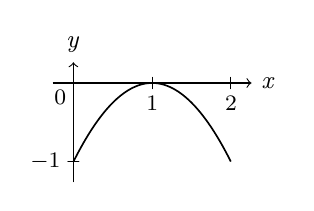
\begin{tikzpicture}
\datavisualization [school book axes,
                    visualize as smooth line,
                    y axis={label},
                    x axis={label} ]

data [format=function] {
      var x : interval [0:2] samples 150;
      func y =  2*\value x -  \value x*\value x - 1 ;
      };
\end{tikzpicture}
 \choice 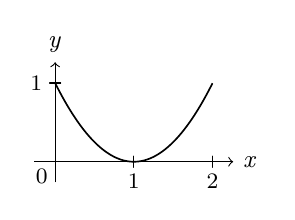
\begin{tikzpicture}
\datavisualization [school book axes,
                    visualize as smooth line,
                    y axis={label},
                    x axis={label} ]

data [format=function] {
      var x : interval [0:2] samples 150;
      func y =   \value x*\value x-2*\value x + 1 ;
      };
\end{tikzpicture}
\choice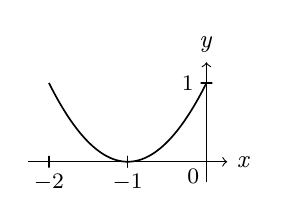
\begin{tikzpicture}
\datavisualization [school book axes,
                    visualize as smooth line,
                    y axis={label},
                    x axis={label} ]

data [format=function] {
      var x : interval [-2:0] samples 150;
      func y =   \value x*\value x+2*\value x + 1 ;
      };
\end{tikzpicture}
 \choice 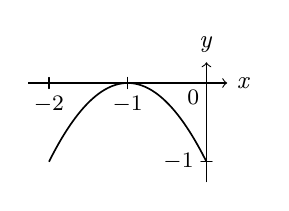
\begin{tikzpicture}
\datavisualization [school book axes,
                    visualize as smooth line,
                    y axis={label},
                    x axis={label} ]

data [format=function] {
      var x : interval [-2:0] samples 150;
      func y =   -\value x*\value x-2*\value x - 1 ;
      };
\end{tikzpicture}
 
\end{oneparchoices}

\question (The value of the determinant) $ \begin{vmatrix}
-8 & 3 & 3\\
3 & -8 & 5\\
5 & 5 & -8
\end{vmatrix} $ নির্নায়কটির মান- 

\begin{oneparchoices}
\choice $ 1 $
\choice $ -1 $
\choice $ 0 $
\choice $ 2 $
\end{oneparchoices}

\question একই বিন্দুতে ক্রিয়ারত 2 একক ও 3 একক মানের দুটি বলের লদ্ধির মান 4 একক। বলদুটির অন্তর্ভুক্ত কোণ কত? (The magnitude of the resultant of two forces acting at a point and having magnitudes 2 units and 3 units. What is the angle between the two forces )

\begin{oneparchoices}
\choice $ \cos^{-1}\Big(\dfrac{1}{4} \Big) $
\choice $ \cos^{-1}\Big(\dfrac{1}{2} \Big) $
\choice $ \cos^{-1}\Big(\dfrac{1}{3} \Big) $
\choice $ \cos^{-1}\Big(\dfrac{1}{5} \Big) $
\end{oneparchoices}

\question  (The value of )  $ \mathlarger{\int_{1}^{e}\ln x\, dx} $ এর  মান (is) – 

\begin{oneparchoices}
\choice  $ e $
\choice  $ e-1 $
\choice  1
\choice  $ 1-e $
\end{oneparchoices}

\question $ \omega $ যদি 1 এর একটি জটিল ঘনমূল হয়, তবে $ (1-\omega +\omega^{2})(1-\omega^{2}+\omega^{4}) $ এর মান – (If $ \omega $ is a complex (imaginary) cube root of unity, thenthe value of $ (1-\omega +\omega^{2})(1-\omega^{2}+\omega^{4}) $ is)
 
\begin{oneparchoices}
\choice $ 4 $
\choice $ 6 $
\choice $ 3 $
\choice $ 2 $
\end{oneparchoices}

\question  নিচের কোন উক্তি সত্য?  (Which of the following statement is true?)

\begin{oneparchoices}
\choice  $ A\setminus B = A\cap B^{\prime} $
\choice  $ A\setminus B = A\cup B^{\prime} $
\choice  $ A\setminus B = A^{\prime}\cap B $
\choice  $ A\setminus B = A^{\prime}\cup B $
\end{oneparchoices}

\question  নিন্মোক্ত রাশিমালার মান-(The value of the following expression $ \sin (780^{\circ})\cos (390^{\circ})-\sin (330^{\circ}) (-300^{\circ})$ is )  

\begin{oneparchoices}
\choice $ -1 $
\choice $ 0 $
\choice $ 1 $
\choice $ \dfrac{1}{2} $
\end{oneparchoices}

\end{questions}

\begin{LARGE}
\begin{center}
গণিত (Mathematics - 2001)
\end{center}
\end{LARGE}
\begin{questions}

\question  প্রক্ষেপকের উত্থানকাল $ t $ সর্বোচ্চ উচ্চতা $ H $ হলে $ \dfrac{H}{t^{2}} $ কত? (If $ t $ is the time of ascent and $ H $ the greatest height attained by a projectile, then $ \dfrac{H}{t^{2}} $ is )

\begin{oneparchoices}
\choice $ \dfrac{1}{2} $
\choice $ 2 $
\choice $ \dfrac{g}{2} $
\choice $ \dfrac{1}{2g} $
\end{oneparchoices}

\question নিচের কোন রাশিমালাটি $ \sin 3A $ কে $ \sin A $ বা $ \cos A $ এর বহুপদী রুপে প্রকাশ করে (Which of the following expression gives  $ \sin 3A $ as a polynomial in $ \sin A $ or $ \cos A $) -

\begin{oneparchoices}
\choice  $ 3\cos A -4\cos^{3} A $
\choice  $ 3\sin A -4\sin^{3} A $
\choice  $ 4\cos^{3} A -3\cos A $
\choice  $ 4\sin^{3} A -3\sin A $
\end{oneparchoices}

\question  $ \cos 420^{\circ}\cos 390^{\circ} + \sin (-300^{\circ})\sin (-330^{\circ}) $ এর মান- (The value of $ \cos 420^{\circ}\cos 390^{\circ} + \sin (-300^{\circ})\sin (-330^{\circ}) $ ) 

\begin{oneparchoices}
\choice  0
\choice  $ -1 $
\choice  1
\choice  $ \dfrac{1}{2} $
\end{oneparchoices}

\question $ x^{2}+y^{2}-6x-4y+c=0 $ বৃত্তটি $ y $ অক্ষকে স্পর্শ করলে $ c $ এর মান কত? (What is the value of $ c $ if the circle $ x^{2}+y^{2}-6x-4y+c=0 $ touches the $ y $ axis )

\begin{oneparchoices}
\choice 11
\choice 7
\choice 5
\choice 4
\end{oneparchoices}

\question $ y=e^{\sqrt{x}} $ হলে $ \dfrac{dy}{dx}=?  $ (If $ y=e^{\sqrt{x}} $ then $ \dfrac{dy}{dx}=?  $) 

\begin{oneparchoices}
\choice $ \dfrac{e^{\sqrt{x}}}{2\sqrt{x}} $
\choice $ \dfrac{e^{x}}{2\sqrt{x}} $
\choice $ \dfrac{e^{\sqrt{x}}}{2x} $
\choice $ \dfrac{e^{\sqrt{x}}}{\sqrt{2x}} $
\end{oneparchoices}

\question কী পরিমাণ বল 40 কেজি ভরের একটি স্থির বস্তুর উপর প্রয়োগ করলে সেকেন্ডে তার বেগ 18 মি/সে. হবে? (What force apply on a stationary body of mass 40kg will make its speed 18m/s on 6 seconds )

\begin{oneparchoices}
\choice 12 N
\choice 24 N
\choice 120 N
\choice 60 N
\end{oneparchoices}

\question যদি $ f(x) = x^{2}+3 $ এবং $ g(x) = \sqrt{x} $ হয় তাহলে $ f(g(x)) = ? $ (If $ f(x) = x^{2}+3 $ and $ g(x) = \sqrt{x} $ then $ f(g(x)) = ? $ )

\begin{oneparchoices}
\choice $ 2x+3,\, x<0 $
\choice $ x^{2}+1 $
\choice $ 3+9x $
\choice $ x+3,\,x\ge 0 $
\end{oneparchoices}

\question $ f(x) = \sqrt{1-\sqrt{x}} $  হলে $ \dfrac{dy}{dx}=?  $ (If $ f(x) = \sqrt{1-\sqrt{x}} $ then $ \dfrac{dy}{dx}=?  $ )

\begin{oneparchoices}
\choice $ \dfrac{-1}{4\sqrt{x(x-\sqrt{x})}} $
\choice $ \dfrac{1}{2\sqrt{x(1-\sqrt{x})}} $
\choice $ \dfrac{1}{x\sqrt{x-1}} $
\choice $ \dfrac{1}{4\sqrt{x-1}} $
\end{oneparchoices}

\question $ x^{2}+y^{2}=25 $ হলে $ (3,-4) $ বিন্দুতে $ \dfrac{dy}{dx} = $ কত? (If $ x^{2}+y^{2}=25 $ then what is the value of $ \dfrac{dy}{dx} $ at point $ (3,-4) $ ? )

\begin{oneparchoices}
\choice $ \dfrac{5}{6} $
\choice $ \dfrac{3}{4} $
\choice $ 0 $
\choice  $ \dfrac{7}{2} $
\end{oneparchoices}

\question  $ (a+b)^{15} $ এর 7-তম সহগ কত? (What is the coefficient of the $ 7^{th} $ term of $ (a+b)^{15} $ ?)

\begin{oneparchoices}
\choice $ 5008 $
\choice $ 5005 $
\choice $ 7009 $
\choice $ 6007 $
\end{oneparchoices}

\question  $ \mathlarger{\int_{0}^{1}}\dfrac{e^{\sqrt{x}}}{\sqrt{x}}dx=? $

\begin{oneparchoices}
\choice  $ 2(e-1) $
\choice  $ 2(e+1) $
\choice  $ 2(1-e) $
\choice  $ e+1 $
\end{oneparchoices}

\question  যদি $ (-5,1),\,(4,5) $ এবং $ (7,-4) $ একটি ত্রিভুজের শীর্ষ বিন্দু হয় তবে তার ক্ষেত্রফল কত? (What is the area of the triangle whose vertices are $ (-5,1),\,(4,5) $ and  $ (7,-4) $ ?)


\begin{oneparchoices}
\choice $ 48\dfrac{1}{2} $
\choice $ 46\dfrac{1}{2} $
\choice $ 50 $
\choice  $ 50\dfrac{1}{2} $
\end{oneparchoices}

\question $ \alpha $ এর কোনমানের জন্য $ (\alpha+1)x+(\alpha +1)y-7=0 $ রেখাটি $ 3x+5y+7=0 $ রেখার সমান্তরাল হবে? (For what value of $ \alpha $ the line $ (\alpha+1)x+(\alpha +1)y-7=0 $ is parallel to the line $ 3x+5y+7=0 $ ? )

\begin{oneparchoices}
\choice $ \alpha = 4 $
\choice $ \alpha = 10 $
\choice $ \alpha = 1 $
\choice $ \alpha = 6 $  
\end{oneparchoices}

\question সাতজন ইংরেজ এবং চারজন মর্কিনিদের মধ্যে থেকে ছয়জনের একটি কমিটি গঠন করতে হবে। কমিটিতে কমপক্ষে দুইজন মর্কিনি থাকবে এইশর্তে এই কমিটি কতপ্রকারে গঠন করা যেতে পারে? (From 7 Englishmen and 4 Americans a committee of 6 is to be formed, in how many ways can this be done when the committee contains at least 2 Americans ?)

\begin{oneparchoices}
\choice $ 350 $
\choice $ 371 $
\choice $ 381 $
\choice $ 415 $
\end{oneparchoices}

\question কোন স্কুলে 120 জন ছাত্রের 75 জন বাংলা ভাষায় এবং 60 জন ইংরেজি অথবা উভয়ভাষায় কথা বলতে পারে। কতজন উভয় ভাষায় কথা বলতে পারে? (In a school out of 120 students, 75 students speak in Bengali and 60 students speak in English or both. How many students speak in both languages?)

\begin{oneparchoices}
\choice $ \dfrac{1}{3} $
\choice $ \dfrac{2}{3} $
\choice $ \dfrac{4}{5} $
\choice $ \dfrac{1}{6} $
\end{oneparchoices}

\question $ 0.6+0.06+0.006+ \cdots \cdots $ অসীম ধারা এর যোগফল কত? (What is the sum of the infinite series $ 0.6+0.06+0.006+ \cdots \cdots $ ? )


\begin{oneparchoices}
\choice $ \dfrac{1}{3} $
\choice $ \dfrac{2}{3} $
\choice $ \dfrac{4}{5} $
\choice $ \dfrac{1}{6} $
\end{oneparchoices}

\question $ \begin{vmatrix}
\beta -2 & 1\\
-5 & \beta +4
\end{vmatrix} $ নির্ণায়কটির মান $ 0 $ হলে $ \beta $ এর মান কত? (What is the value of the determinant $ \begin{vmatrix}
\beta -2 & 1\\
-5 & \beta +4
\end{vmatrix} $ is 0 then what is the value of $ \beta $ ? )


\begin{oneparchoices}
\choice 5 or 0
\choice 6 or 2 
\choice 5 or $ -5 $
\choice 1 or $ -3 $
\end{oneparchoices}

\question $ |2x-7|>5 $ অসমতাটির বাস্তব সংখ্যায় সমাধান কি? (What is the solution of the inequality $ |2x-7|>5 $ in real numbers?)


\begin{oneparchoices}
\choice $ x<1 $
\choice $ x>6 $
\choice $ x>6 $ or $ x<1 $
\choice $ x>6 $ and $ x<1 $
\end{oneparchoices}

\question $ \vec{A} = \hat{i}-2\hat{j}+3\hat{k} $ এবং $ \vec{B} = 2\hat{i}+\hat{j}-\hat{k} $ হলে $ A*B=? $ (If $ \vec{A} = \hat{i}-2\hat{j}+3\hat{k} $ and $ \vec{B} = 2\hat{i}+\hat{j}-\hat{k} $ then  $ A*B=? $)

\begin{oneparchoices}
\choice  $ -3 $
\choice  $ -2 $
\choice  $ 2 $
\choice  $ 3 $
\end{oneparchoices}

\question একটি বাক্সে 10টি নীল ও 15টি সবুজ মার্বেল আছে। দৈব চয়ন পদ্ধতিতে একটির পর আরেকটি মোটদুটি মার্বেল নেয়া হলে মার্বেল দুটি ভিন্ন রংয়ের হওয়ার সম্ভাবনা কত? (A box contains 10 blue and 15 green marbles, one after another, two marbles are drawn at random from the box. What is the probability that they have different colours?  )


\begin{oneparchoices}
\choice $ \dfrac{1}{4} $
\choice $ \dfrac{3}{5} $
\choice $ \dfrac{1}{2} $
\choice  $ \dfrac{2}{5} $
\end{oneparchoices}

\question $ x^{2}-5x-3= 0 $ সমীকরণের মূলদ্বয় $ x_{1},x_{2} $ হলে $ \dfrac{1}{x_{1}},\dfrac{1}{x_{2}} $ মূল বিশিষ্ট সমীকরণটি কত? (If $ x_{1},x_{2} $ be the roots of the equation $ x^{2}-5x-3= 0 $. What is the equation whose roots are $ \dfrac{1}{x_{1}},\dfrac{1}{x_{2}} $? )


\begin{oneparchoices}
\choice $ 3x^{2}-5x+1= 0 $
\choice $ 5x^{2}+x-3= 0 $
\choice $ 3x^{2}+5x-1= 0 $
\choice $ 5x^{2}-x-3= 0 $
\end{oneparchoices}

\question $ \omega $ যদি 1 এর একটি জটিল ঘনমূল হয়, তবে $ (1-\omega +\omega^{2})^{2}+(1-\omega^{2}+\omega)^{2} $ এর মান – (If $ \omega $ is a complex (imaginary) cube root of unity, then the value of $ (1-\omega +\omega^{2})^{2}+(1-\omega^{2}+\omega)^{2} $ is)
 
\begin{oneparchoices}
\choice $ 4 $
\choice $ -4 $
\choice $ 3 $
\choice $ -3 $
\end{oneparchoices}

\question 3P এবং 4P মানের দুটি বল পরস্পর লম্বভাবে ক্রিয়া করে। তাদের লদ্ধির মান কত? (Two forces of magnitudes 3P and 4 P act at a point making right angle to each other. What is the resultant of the forces ?)


\begin{oneparchoices}
 \choice $ \sqrt{43}\,P $
 \choice $ 9\,P $
 \choice $ 2\sqrt{2}\,P $
 \choice $ \sqrt{35}\,P $
\end{oneparchoices}

\question  $ y^{2} = 4x+8y $ পরাবৃত্তটির শীর্ষ বিন্দুর স্থানাংক কত? (What are the coordinates of the vertex of the parabola $ y^{2} = 4x+8y $ ?)

\begin{oneparchoices}
\choice $ (-4,4) $
\choice $ (4,4) $
\choice $ (4,-4) $
\choice $ (-4,-4) $
\end{oneparchoices}

\question $ \dfrac{2\tan\theta}{1+\tan^{2}\theta} =? $

\begin{oneparchoices}
\choice $ \tan 2\theta $
\choice $ 2\sin \theta\cos \theta $
\choice $ 2\cos^{2}\dfrac{\theta}{2} $
\choice $ \cos 2\theta $
\end{oneparchoices}

\end{questions}

\end{document}